\documentclass[12pt]{report}
\usepackage{graphicx}
\usepackage{amssymb,amsmath,amsfonts}
\usepackage[spanish,es-tabla]{babel}
\usepackage[ansinew]{inputenc}
\usepackage[colorlinks=true,urlcolor=blue,linkcolor=blue]{hyperref}
\usepackage{graphicx}
\usepackage{geometry} 
\usepackage{fancyhdr}
\usepackage{floatrow}
\usepackage{xcolor}
\usepackage{listings}
\usepackage{tcolorbox}
\usepackage{amsthm}
% Definir el entorno para ejemplos con texto en roman (no it�lico)
\newtheorem{example}{Ejemplo}[chapter]
% Redefinir el entorno para que use normalfont en lugar de it�lica
\makeatletter
\def\th@plain{\normalfont} % Cambiar el estilo del cuerpo del texto a normalfont
\makeatother
% Comando para la l�nea personalizada
\newcommand{\exampleline}{
\par\noindent
\textcolor{red}{\rule{0.25\linewidth}{0.8pt}}
}
%\usepackage{draftwatermark}
%\SetWatermarkText{Borrador Preliminar}
%\SetWatermarkScale{3.5}
%New colors defined below
\definecolor{codegreen}{rgb}{0,0.6,0}
\definecolor{codegray}{rgb}{0.5,0.5,0.5}
\definecolor{codepurple}{rgb}{0.58,0,0.82}
\definecolor{backcolour}{rgb}{0.95,0.95,0.92}
\definecolor{ghostwhite}{rgb}{0.97, 0.97, 1.0}
%Code listing style named "mystyle"
\lstdefinestyle{mystyle}{
  backgroundcolor=\color{backcolour}, commentstyle=\color{codegreen},
  keywordstyle=\color{magenta},
  numberstyle=\tiny\color{codegray},
  stringstyle=\color{codepurple},
  basicstyle=\ttfamily\footnotesize,
  breakatwhitespace=false,         
  breaklines=true,                 
  captionpos=b,                    
  keepspaces=true,                 
  numbers=left,                    
  numbersep=5pt,                  
  showspaces=false,                
  showstringspaces=false,
  showtabs=false,                  
  tabsize=2
}
%"mystyle" code listing set para las cajitas de c�digo
\lstset{style=mystyle}
\setlength{\topmargin}{-0.25in}
\setlength{\textheight}{10in}
\setlength{\textwidth}{6.8in}
\setlength{\oddsidemargin}{-0.5in}
\usepackage{booktabs}
%%%%%%%%%%%%%%%%%%%%%%

\setlength{\topmargin}{-1.0in}
\setlength{\textheight}{9in}
\setlength{\textwidth}{6.8in}
\setlength{\oddsidemargin}{-0.5in}

\begin{document}
\begin{figure}
\raggedright
{
\includegraphics[width=60mm]{figuras/logouis}} 
\end{figure}

\title{\bf Gu�a general para el laboratorio de F�sica}
\author{H�ctor F. Hern�ndez G.}
\date{Versi�n 3.0 -  \today }


\maketitle
\newpage
\thispagestyle{empty}
\setcounter{page}{1}
\pagenumbering{roman}

\pagestyle{plain}

\tableofcontents
\pagenumbering{arabic}
\setcounter{page}{1}

\chapter{Mediciones en el laboratorio}

\section{Introducci�n}

En este cap�tulo, se abordar�n los conceptos fundamentales relacionados con las mediciones en el contexto del laboratorio de f�sica. Se explorar�n las unidades de medida, los instrumentos comunes utilizados para medir diferentes magnitudes y las t�cnicas b�sicas para llevar a cabo mediciones precisas.

En el entorno del laboratorio de f�sica, los objetivos se centran en la realizaci�n precisa y eficiente de experimentos, as� como en el desarrollo de habilidades clave para la investigaci�n cient�fica. Estos objetivos incluyen:

\begin{itemize}
\item  Obtenci�n de Mediciones Precisas: El primer objetivo es llevar a cabo experimentos f�sicos con el fin de obtener valores precisos de las cantidades f�sicas medidas.

\item Elaboraci�n y An�lisis de Gr�ficos: Un segundo objetivo es adquirir la habilidad de crear gr�ficos adecuados y analizar la informaci�n cient�fica que estos gr�ficos contienen. Esto es esencial para visualizar y comprender los resultados de manera efectiva.

\item Redacci�n de Informes de Laboratorio: La correcta redacci�n de informes de laboratorio es fundamental en la comunicaci�n de resultados cient�ficos. Por lo tanto, otro objetivo importante es aprender a redactar informes de laboratorio de manera precisa y coherente.

\item Exploraci�n de Nuevos T�picos de la F�sica: El laboratorio tambi�n cumple la funci�n de introducir a los estudiantes en nuevos conceptos y t�picos de la f�sica que pueden no haber sido tratados en las clases te�ricas.
\end{itemize}

Adem�s, es importante destacar que, mientras las clases te�ricas suelen presentar experimentos de manera cualitativa, el laboratorio se enfoca en la realizaci�n cuantitativa de los mismos. En este contexto, surgen preguntas inevitables, como: �cu�l es la precisi�n y exactitud alcanzada en una medici�n?, �cu�l es la precisi�n y exactitud que se podr�a lograr?, y �qu� conceptos f�sicos se aplican y qu� condiciones deben cumplirse?

En los cap�tulos siguientes, se abordar�n estas preguntas y se presentar�n conceptos clave relacionados con la teor�a de errores, el tratamiento de datos y el an�lisis gr�fico.

\section{Mediciones}

El trabajo en el laboratorio implica medir magnitudes f�sicas mediante la utilizaci�n de instrumentos de medida.

Medir es la comparaci�n de la magnitud que se est� estudiando con un patr�n de medida. Si cada persona tuviera su propio patr�n de medida, solo �l comprender�a el valor de su resultado y no podr�a establecer comparaciones, a menos que supiera la equivalencia entre su patr�n y el de su vecino. Por esta raz�n se ha acordado el establecimiento de un patr�n. Si bien hasta hace poco, algunos pa�ses utilizaban como sistema de unidades el Sistema Brit�nico, y otros pa�ses el Sistema M�trico Decimal, la tendencia es usar el Sistema Internacional (SI) \footnote{\url{https://es.wikipedia.org/wiki/Sistema_Internacional_de_Unidades}}.

El Sistema Internacional de Unidades (SI) se apoya en las siguientes magnitudes b�sicas:
$$
\begin{array}{ccc}
\text { S�mbolo } & \text { Nombre } & \text { Magnitud } \\ \hline \hline 
\text { s } & \text { segundo } & \text { tiempo } \\
\text { m } & \text { metro } & \text { longitud } \\
\text { kg } & \text { kilogramo } & \text { masa } \\
\text { A } & \text { amperio } & \text { corriente el�ctrica } \\
\text { K } & \text { kelvin } & \text { temperatura termodin�mica } \\
\text { mol } & \text { mol } & \text { cantidad de sustancia } \\
\text { cd } & \text { candela } & \text { intensidad luminosa }
\end{array}
$$

Se puede decir que el resultado de una medida es lo que se conoce como el valor de la magnitud. Este valor debe ir siempre acompa�ado de su respectiva unidad de medida. Decir que la masa de una varilla es de $80,4$ no significa nada, se preguntar�: �$80,4$ gramos?, �$80,4$ libras?, �$80,4$ kilogramos?, �qu� dir�a Ud. si en un almac�n de telas le venden un pie de tela y le cobran un metro? �Ah! entonces es importante que las cantidades que se midan vayan acompa�adas de sus respectivas unidades de medida.

$$
\begin{aligned}
& \text { Cuadro 1.1: Unidades b�sicas utilizadas en mec�nica } \\
& \begin{array}{|c|c|c|c|}
\hline \text { Magnitudes } & \text { SI } & \text { CGS } & \text { brit�nico } \\
\hline \hline \text { Longitud } & \text { Metro (m) } & \text { Cent�metro (cm) } & \text { Pie (ft) } \\
\hline \text { Masa } & \text { Kilogramo }(\mathrm{kg}) & \text { Gramo }(\mathrm{g}) & \text { Libra }(\mathrm{lb}) \\
\hline \text { Tiempo } & \text { Segundo }(\mathrm{s}) & \text { Segundo }(\mathrm{s}) & \text { Segundo }(\mathrm{s}) \\
\hline
\end{array}
\end{aligned}
$$

El sistema CGS es el Sistema Cegesimal de Unidades o sistema gaussiano, es un sistema de unidades basado en el cent�metro, el gramo y el segundo y el sistema brit�nico es un conjunto de unidades de medida diferentes a las del sistema m�trico decimal, que se utilizan actualmente como medida principal en los Estados Unidos y el Reino Unido.

En la actualidad los instrumentos de medici�n pueden encontrarse en formato anal�gico o digital, figura \ref{anadigi}. Los instrumentos anal�gicos suelen requerir de cierta pr�ctica para leer las mediciones, mientras que los instrumentos digitales presentan las lecturas directamente en una pantalla. Dependiendo del objeto a medir se puede preferir un instrumento de medici�n anal�gico a uno digital. 
\begin{figure}[!h]
\begin{center}
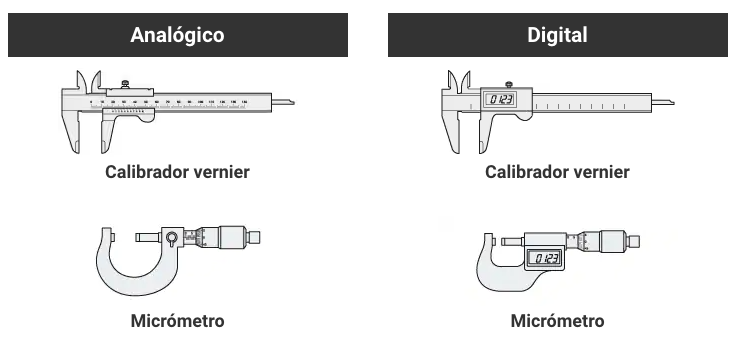
\includegraphics[height=2.2in,width=4.4in]{figuras/fig01}  
\caption{Instrumentos de medida anal�gicos y digitales}
\label{anadigi}
\end{center}
\end{figure}

Los instrumentos de medida nos muestran el valor de las medidas dentro de cierto rango de validez que es caracter�stico del propio aparato de medida. 

\paragraph{Apreciaci�n:} La menor divisi�n en la escala de cualquier instrumento de medida se llama {\it apreciaci�n}. En instrumentos anal�gicos cuando se lee en una escala �nica, se  aproxima la lectura a la divisi�n m�s cercana. Por esto, el m�ximo error que se puede cometer en dicha medici�n es de $\pm$ la apreciaci�n.

Por lo anterior cualquier medida nunca es exacta, su �ltima cifra siempre es aproximada, debido a ello toda medida presenta siempre una incertidumbre o error determinada por la precisi�n del instrumento.

La determinaci�n de la apreciaci�n de un instrumento que tiene solamente una escala anal�gica, se realiza siguiendo la explicaci�n dada a continuaci�n.

Se escogen dos valores sobre la escala, que pueden ser consecutivos o no. Se hace la diferencia del valor mayor $n$ menos el valor menor $m$ y se divide entre el n�mero de partes en que est� dividido el intervalo (ver figura \ref{aprecia}).
$$
\text { Apreciaci�n }=\frac{n-m}{\text {N}^0 \text { total de divisiones }}
$$
\begin{figure}[h]
\begin{center}
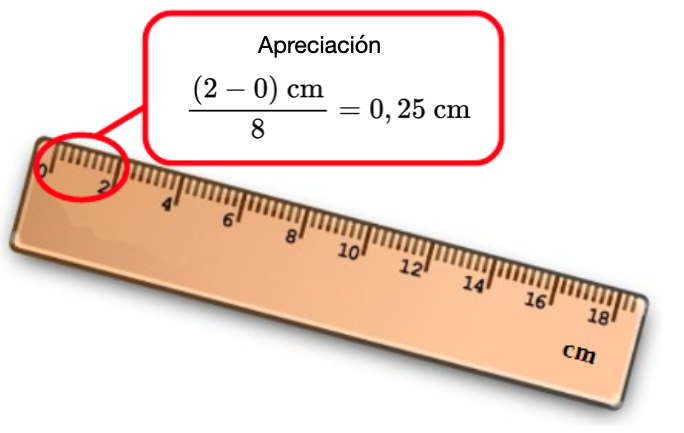
\includegraphics[height=1.8in,width=3.0in]{figuras/fig02}  
\caption{Apreciaci�n de un instrumento}
\label{aprecia}
\end{center}
\end{figure}

La apreciaci�n de un instrumento es una indicaci�n del error de la medida, se habla entonces de "precisi�n" de un instrumento o de la sensibilidad: a menor apreciaci�n, mayor precisi�n.


\subsection{Medici�n de la masa}

En el Sistema Internacional (SI), la unidad para medir la masa es el kilogramo (kg), con sus derivadas como el gramo y el miligramo. Para medir la masa de un objeto, se utilizan balanzas o b�sculas. Algunos tipos de balanzas incluyen:
\begin{itemize}
\item Balanza de dos platillos: compara la masa desconocida con masas conocidas en dos platillos.

\item Balanza de un solo platillo: el objeto se coloca en un platillo y se ajusta el equilibrio con jinetillos en una escala graduada. Pueden ser mec�nicas o electr�nicas.

\item Balanza anal�tica: dise�ada para medir masas muy peque�as, con precisi�n de hasta la diezmil�sima de gramo (0,0001 g o 0,1 mg).
\end{itemize}

Al usar una balanza, se deben seguir algunas reglas:
\begin{itemize}
\item Manejarlas con cuidado, especialmente las electr�nicas.
\item Evitar tocar el platillo con los dedos.
\item  No poner sustancias qu�micas o recipientes h�medos directamente en el platillo, utilizar papel.
\end{itemize}

\subsection{Medici�n de la longitud}

La longitud se mide en metros (m) y sus m�ltiplos y subm�ltiplos seg�n el Sistema Internacional de Unidades (SI). Para medir longitudes enormes, como las del espacio exterior, se utilizan unidades especiales:
\begin{itemize}
\item A�o luz (ly): Distancia que recorre la luz en un a�o, aproximadamente 9,46 billones de kil�metros.
\item Unidad Astron�mica (UA): Distancia media entre la Tierra y el Sol, aproximadamente 149,6 millones de kil�metros.
\item P�rsec (pc): Equivalente a 206.264,81 UA.
\end{itemize}

\subsubsection{La regla o cinta m�trica}
El instrumento m�s com�n para medir longitudes es la cinta m�trica, con una apreciaci�n de 1 mm. La medici�n de la longitud de un objeto implica una comparaci�n directa con una cinta m�trica. Para llevar a cabo esta medici�n, debemos fijar la posici�n de los extremos del objeto sobre la escala graduada de la cinta m�trica. Es aconsejable colocar el objeto de manera que sea f�cil de leer con claridad, como se muestra en la figura \ref{regla}. \begin{figure}[h]
\begin{center}
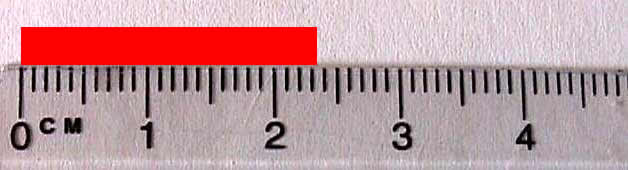
\includegraphics[height=1.2in,width=3.8in]{figuras/fig02a}  
\caption{Forma correcta de medir con una regla. Medida: (2,3 $\pm$ 0,1) cm.}
\label{regla}
\end{center}
\end{figure}

La medici�n de un objeto con una regla graduada o una cinta m�trica puede llevar a una fracci�n de la escala que no puede ser apreciada, como se muestra en la figura \ref{regla}, donde el objeto mide entre 2,3 cm y 2,4 cm.

\subsubsection{El vernier}

El vernier permite medir con mayor precisi�n que una regla graduada. Su apreciaci�n se calcula como la diferencia entre la longitud de una divisi�n de la escala principal y una del nonio. Por ejemplo, un vernier con una apreciaci�n de 0,005 mm permitir�a una lectura de 2,355 mm.

En la figura \ref{vernier} de la izquierda podemos ver un vernier midiendo una esfera dando una lectura de $1.640 \pm 0.005$.
\begin{figure}[!h]
\begin{center}
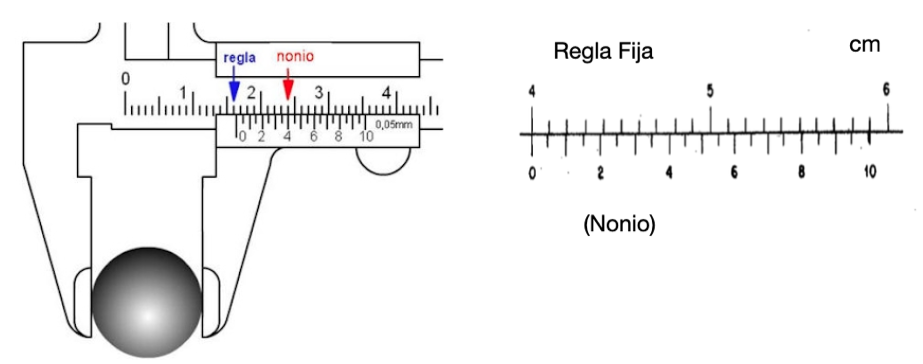
\includegraphics[height=2.0in,width=3.0in]{figuras/fig02b}  \quad 
\includegraphics[height=1.4in,width=2.6in]{figuras/fig02c}  
\caption{Izquierda: Vernier mostrando una medida de (1.640 $\pm$ 0,005) cm. Derecha: escalas del vernier}
\label{vernier}
\end{center}
\end{figure}

El vernier consta de dos partes principales: una escala principal con divisiones milim�tricas y una escala m�vil, el nonio, generalmente graduado en 10 o 20 divisiones. En la figura \ref{vernier}, el nonio tiene 20 divisiones. La apreciaci�n del vernier se calcula como la diferencia entre la longitud de una divisi�n de la escala principal y la longitud de una divisi�n del nonio.

Para el caso general, cuando el nonio tiene $n$ divisiones, la apreciaci�n del vernier se puede determinar de la siguiente manera:
$$
\text {Apreciaci�n del vernier }=\frac{\text {Apreciaci�n de la escala principal }}{\text{N}^0 \text { total de divisiones del nonio }} \,.
$$

Para el vernier de la figura \ref{vernier}, la apreciaci�n es:
$$
\text {Apreciaci�n }=\frac{0,1 \mathrm{~cm}}{20}=0,005 \mathrm{~cm}=0,05 \mathrm{~mm}
$$

Cuando el cero del nonio se coloca, por ejemplo, en la divisi�n $4 \mathrm{~cm}$ de la regla fija, como se muestra en la figura derecha de \ref{vernier}, las divisiones del nonio llegan a $5.9 \mathrm{~cm}$. Esto significa que las 20 divisiones del vernier corresponden a una longitud de $1.9 \mathrm{~cm}$ en la escala principal. Por lo tanto, cada divisi�n del vernier mide $\frac{1.9}{20} \mathrm{~cm}=0.095 \mathrm{~cm}$. La lectura ser�a 4,095 cm.

Volviendo a la figura \ref{vernier}, izquierda,   la posici�n del cero del vernier est� entre $1,6$ y $1,7 \mathrm{~cm}$, es decir, las dos primeras cifras son las que corresponden a la medida hecha  con una cinta m�trica: $1,6 \pm 0,1 \mathrm{~cm}$. La siguiente  cifra   se obtiene del nonio, en este caso la raya 4 del nonio coincide con la raya 2,4 de la escala principal. Entonces la medida que se lee en el vernier ser� $1,6 + 0,040 = 1,640 \mathrm{~cm}$, por lo que el resultado correcto es $(1,640 \pm 0,005) \mathrm{~cm}$, o bien, $(16,40 \pm 0,05) \mathrm{~mm}$.

En la figura \ref{vernier2}, se presenta otro ejemplo de lectura de una medici�n realizada con el vernier. En este caso, a la izquierda del cero del nonio hay 3 divisiones, lo que equivale a 3 mm enteros. En el nonio, la divisi�n que est� justo entre el cuatro y el cinco coincide con una divisi�n de la regla, es decir, 0.45 mm. Por lo tanto, la medida resulta en 3  + 0.45 mm = 3.45 mm.
\begin{figure}[h]
\begin{center}
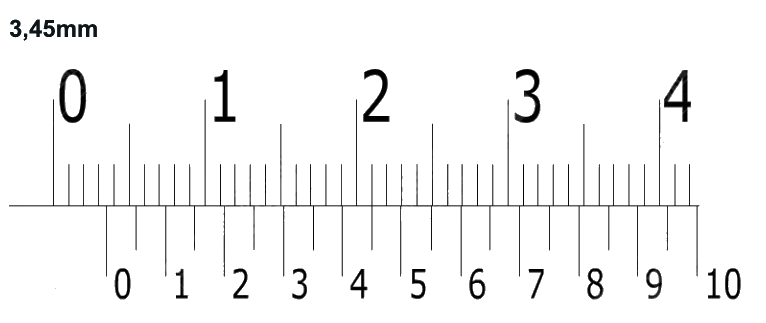
\includegraphics[height=1.4in,width=3.0in]{figuras/fig02d} 
\caption{Medida (3.45 $\pm$ 0,05) mm.}
\label{vernier2}
\end{center}
\end{figure}


\subsubsection{El tornillo microm�trico}

Cuando se utiliza un tornillo que se enrosca en una tuerca, este avanza una distancia determinada con cada giro completo, conocida como el paso del tornillo. Este principio es la base del funcionamiento del Tornillo Microm�trico, un instrumento de precisi�n utilizado para medir longitudes. La figura izquierda de la Figura \ref{tornillo1} muestra un tornillo microm�trico con sus componentes clave, que incluyen la escala fija graduada, el tambor, la tuerca de seguridad y el freno.

La medici�n con el tornillo microm�trico comienza con la lectura de las cifras en la escala fija. Por ejemplo, en la figura derecha de la Figura \ref{tornillo1}, la lectura se obtiene al sumar la lectura de la escala fija con la del tambor, resultando en este caso:  5 + 0,5 + 0,28 = 5,78  mm. 

Para comprender esta lectura, es importante tener en cuenta que el tornillo tiene un paso de 0,5 mm, y el tambor est� dividido en 50 partes iguales, lo que equivale a una apreciaci�n de 0,01 mm.

La apreciaci�n de un tornillo microm�trico se calcula utilizando la f�rmula:
\[
\text{Apreciaci�n} = \frac{\text{paso del tornillo}}{\text{N�mero total de divisiones del tambor}}.
\]

En el caso del tornillo de la Figura \ref{tornillo1}, la apreciaci�n es de:
\[
\text{Apreciaci�n} = \frac{0,5 \mathrm{~mm}}{50} = 0,01 \mathrm{~mm}.
\]
Por lo tanto, la lectura en esta figura se expresa como $(5,78 \pm 0,01) \mathrm{mm}$.
\begin{figure}[h]
\begin{center}
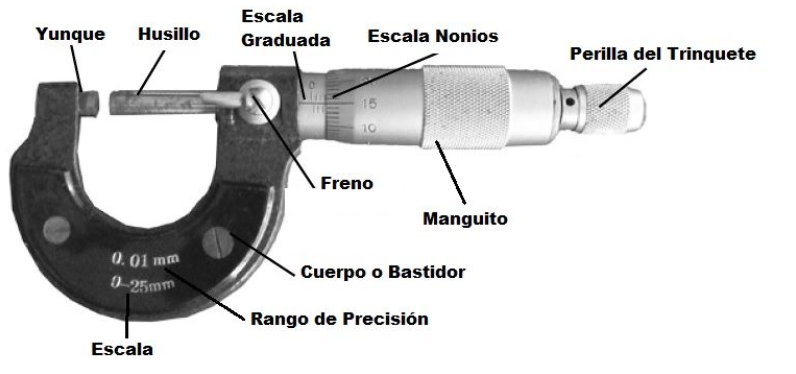
\includegraphics[height=1.6in,width=3.0in]{figuras/fig02e1} 
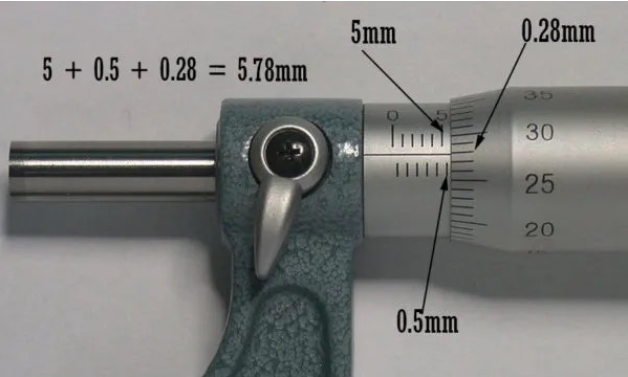
\includegraphics[height=1.6in,width=3.0in]{figuras/fig02e2} 
\caption{Tornillo Microm�trico}
\label{tornillo1}
\end{center}
\end{figure}

Adem�s, cabe mencionar que en la escala fija milim�trica se incluyen divisiones en la parte inferior que facilitan determinar si el tambor ha dado una vuelta completa, indicando la necesidad de agregar $0,50 \mathrm{~mm}$ a la lectura del tambor.

\subsection{Medici�n del tiempo}

En f�sica, el tiempo es una magnitud que se utiliza para medir la duraci�n o la separaci�n de uno o m�s acontecimientos. Su unidad de medici�n en el Sistema Internacional es el segundo (s), y 60 de estas unidades constituyen una unidad mayor llamada minuto (min). Los aparatos con los que se mide el tiempo son el reloj o el cron�metro.

\subsubsection{El cron�metro}

Los intervalos de tiempo se pueden medir utilizando un cron�metro, que, seg�n la tecnolog�a utilizada en su construcci�n, puede ser de reloj digital o anal�gico. Por lo general, indican el tiempo en minutos, segundos y fracciones de segundo. Cuentan con un bot�n utilizado para iniciar y detener el cronometraje, as� como otro bot�n para regresar la lectura a cero (ver figura \ref{cronos}).
\begin{figure}[h]
\centering
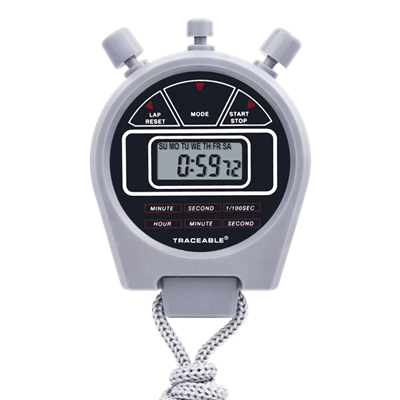
\includegraphics[height=2.0in,width=2.0in]{figuras/fig02f1} \quad 
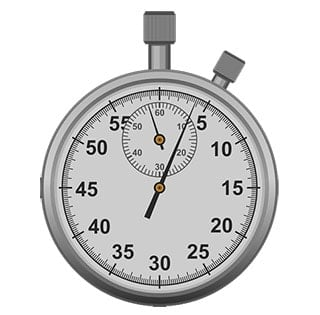
\includegraphics[height=1.8in,width=1.8in]{figuras/fig02f2}
\caption{Cron�metro digital (izquierda) y anal�gico (derecha)}
\label{cronos}
\end{figure}
El cron�metro digital es m�s confiable si deseamos medir tiempos con precisi�n en escalas de mil�simas o cent�simas de segundo. A diferencia de los cron�metros anal�gicos, este tipo de instrumentos se basa en tecnolog�as m�s modernas, que incluyen osciladores de cuarzo y circuitos electr�nicos sofisticados.


\subsection{Medici�n de la temperatura}

La temperatura es una magnitud f�sica que se mide utilizando un term�metro. Existen varias escalas de temperatura, siendo las m�s comunes:

\begin{itemize}
    \item \textbf{Escala Celsius (�C):} En esta escala, el punto de congelaci�n del agua es 0 �C, y su punto de ebullici�n es 100 �C.
    
    \item \textbf{Escala Fahrenheit (�F):} Utilizada en muchos pa�ses de habla inglesa, donde el punto de congelaci�n del agua es 32 �F y su punto de ebullici�n es 212 �F.
    
    \item \textbf{Escala Kelvin (K):} Empleada en la ciencia, establece el "cero absoluto" en -273.15 �C, donde un objeto no desprende calor alguno.
\end{itemize}

Estas escalas se basan en diferentes puntos de referencia y sustancias termom�tricas para su definici�n, pero la Celsius y la Fahrenheit son las m�s comunes en el uso cotidiano.


\subsubsection{El term�metro}

La medici�n directa de la temperatura de un objeto se realiza utilizando un instrumento conocido como term�metro. Los term�metros pueden ser de tipo anal�gico o digital, como se muestra en la figura \ref{termos}. Adem�s, existen term�metros que no requieren contacto f�sico, como los term�metros infrarrojos, �pticos o de radiaci�n. Tambi�n hay otros tipos de term�metros, como los de gas y de resistencia.
\begin{figure}[h]
\begin{center}
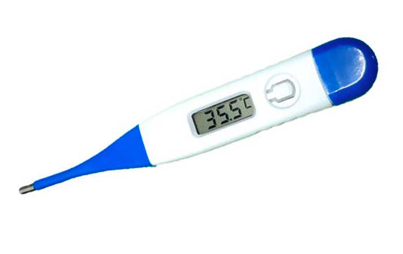
\includegraphics[height=1.4in,width=1.8in]{figuras/fig02g2} \quad
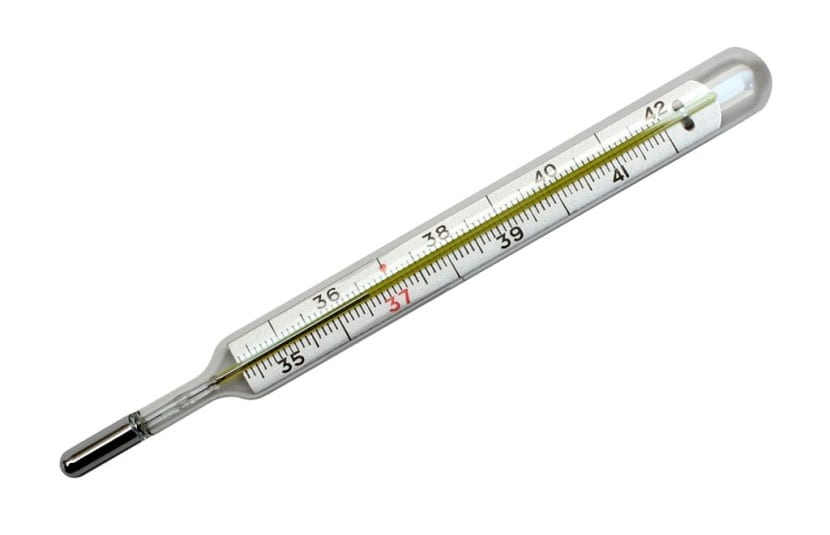
\includegraphics[height=1.4in,width=1.8in]{figuras/fig02g1}
\caption{Term�metro digital (izquierda) y anal�gico (derecha)}
\label{termos}
\end{center}
\end{figure}

Un term�metro t�pico consta de un bulbo de vidrio que contiene un l�quido que experimenta dilataci�n lineal con la temperatura, junto con un tubo capilar graduado y calibrado. El l�quido m�s com�nmente utilizado en term�metros es el mercurio (Hg), debido a su capacidad de dilataci�n regular y su buena conductividad t�rmica.

La escala de un term�metro suele estar dividida por el fabricante, quien garantiza su precisi�n. La apreciaci�n de un term�metro se puede determinar utilizando el m�todo descrito anteriormente para instrumentos con una sola escala. Las escalas de temperatura pueden estar en grados cent�grados (�C), grados Fahrenheit (�F) o kelvins (K, escala absoluta).

La relaci�n entre la escala cent�grada y la escala absoluta (kelvin) es:
\[
T(\mathrm{K}) = T\left({ }^{\circ} C\right) + 273.2
\]
Y la relaci�n entre la escala cent�grada y la escala Fahrenheit es:
\[
T\left({ }^{\circ} F\right) = \frac{9}{5} T\left({ }^{\circ} C\right) + 32
\]

Es importante recordar que un cambio de temperatura de un grado kelvin es equivalente a un cambio de un grado cent�grado, pero un cambio de un grado cent�grado no es igual a un cambio de un grado Fahrenheit.

\subsection{Medici�n de corriente el�ctrica}

La intensidad de la corriente el�ctrica est� relacionada con el flujo de cargas el�ctricas a trav�s de un material conductor por unidad de tiempo. B�sicamente, medimos dos tipos de corriente el�ctrica: la corriente continua y la corriente alterna. La corriente continua circula siempre en el mismo sentido y tiene un valor constante, se produce por pilas o bater�as, y la corriente alterna es corriente que circula en forma oscilatoria. Este tipo de corriente es la que usamos para encender la luz o al enchufar los electrodom�sticos del hogar. La forma m�s com�n de medir la corriente el�ctrica es con un amper�metro, que es un dispositivo que se conecta al circuito el�ctrico e indica los Amperios, que es la unidad de medida seg�n el Sistema Internacional de Unidades (SI) que tiene dicho objeto.

\subsubsection{Amper�metros}

El amper�metro es el instrumento utilizado para medir la corriente en amperios (A) en un circuito. Para la medici�n directa, el amper�metro se conecta en serie con el circuito en el que se va a medir la corriente. Un amper�metro suele tener una resistencia baja para que no produzca una ca�da de tensi�n significativa en el circuito que se est� midiendo.

Los instrumentos utilizados para medir corrientes m�s peque�as, en el rango de los miliamperios o microamperios, se denominan miliamper�metros o microamper�metros, respectivamente.

Existen varios tipos de amper�metros, con tecnolog�as digitales o anal�gicas,  ver figura  \ref{ampes}. 

\begin{itemize}
\item \textbf{Amper�metros magnetoel�ctricos o de bobina m�vil:} Est�n formados por un im�n permanente fijo y un cuadro o bobina m�vil que gira bajo el efecto de la fuerza de Amp�re cuando circula corriente por el mismo. La espiral en el eje del cuadro impide la rotaci�n del cuadro. Cuanto mayor sea la corriente que atraviesa el cuadro, mayor ser� el �ngulo de la aguja cuyo extremo se traslada por una escala.

\item \textbf{Amper�metros electromagn�ticos o de im�n m�vil:} Constan de una aguja unida a un im�n alojado en el interior de una bobina. Cuando la corriente circula por esta �ltima, se produce un campo magn�tico que, dependiendo de su sentido, produce una atracci�n o repulsi�n del im�n que es proporcional a la intensidad de dicha corriente.

\item \textbf{Amper�metros electrodin�micos:} Constan de dos bobinas, una fija y otra m�vil que producen campos magn�ticos, cada una de las cuales porta una corriente que es funci�n de la corriente a medir. La reacci�n entre los campos de la bobina fija y la bobina m�vil proporciona el torque del sistema m�vil, que es compensado por resortes espirales que tambi�n se emplean para llevar la corriente a la bobina m�vil.

\item \textbf{Amper�metros digitales:} Estos aparatos ofrecen la lectura de la corriente directamente en una pantalla eliminando en gran medida los errores de lectura. Se diferencian de los anal�gicos en que las partes mec�nicas m�viles se han sustituido por circuitos electr�nicos, con la gran ventaja de eliminar el desgaste de las partes.
\end{itemize}
\begin{figure}[h]
  \centering
  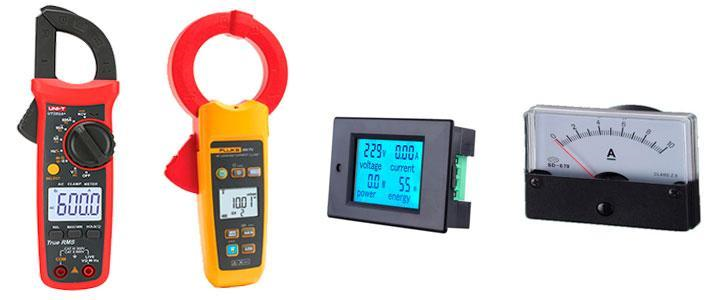
\includegraphics[height=1.8in,width=4.0in]{figuras/fig02h}
  \caption{Diferentes tipos de amper�metros}
  \label{ampes}
\end{figure}


\subsection{Medici�n de la cantidad de sustancia}

La cantidad de sustancia (s�mbolo: $n$) en una muestra dada de materia se define como la relaci�n $n=N / N_{\mathrm{A}}$ entre el n�mero de entidades elementales $N$ y la constante de Avogadro $N_{\mathrm{A}}$. 

Las entidades pueden ser mol�culas, �tomos o iones de un tipo espec�fico. La sustancia concreta que se toma como muestra puede especificarse utilizando un sub�ndice, por ejemplo, la cantidad de cloruro de sodio $(\mathrm{NaCl})$ se denotar�a como $n_{\mathrm{NaCl}}$. 

La unidad de cantidad para la sustancia en el Sistema Internacional de Unidades se denomina mol (s�mbolo: mol). Desde 2019, el valor de la constante de Avogadro $N_{\mathrm{A}}$ se define exactamente como $6,02214076  \times 10^{23} \mathrm{~mol}^{-1}$. A veces, la cantidad de sustancia se denomina cantidad qu�mica.


\subsection{Medici�n de la intensidad luminosa}

La intensidad luminosa es una medida de la potencia ponderada en funci�n de la longitud de onda emitida por una fuente luminosa en una direcci�n determinada por unidad de �ngulo s�lido, basada en la funci�n de luminosidad y normalizada para la sensibilidad del ojo humano. La unidad SI de intensidad luminosa es la candela (cd). En la medici�n de la luz, se distinguen varias magnitudes fotom�tricas con las que se puede evaluar la luz:

\begin{itemize}
\item L�men (lm): Un lumen es la cantidad de energ�a visible que podemos realmente medir. Es el flujo luminoso, una medida de la potencia luminosa emitida por la fuente.
\item Lux (lx): Un lux es el equivalente a la energ�a producida por un lumen que incide sobre una superficie de 1 $\mathrm{m}^2$. Es el nivel de iluminaci�n de una fuente.
\item Candela (cd): La candela consiste en la unidad b�sica que mide la intensidad luminosa. Se define como la intensidad luminosa que va en una direcci�n dada, por lo que se relaciona con el �ngulo de apertura hacia la luz.
\end{itemize}

Para poder medir la luminancia se utiliza un instrumento denominado lux�metro, como se muestra en la figura \ref{luxi}. Un lux�metro permite medir simple y r�pidamente la iluminancia real y no subjetiva de un ambiente. Contiene una c�lula fotoel�ctrica que capta la luz y la convierte en impulsos el�ctricos, los cuales son interpretados y representados en un display o aguja con la correspondiente escala de luxes.
\begin{figure}[h]
\begin{center}
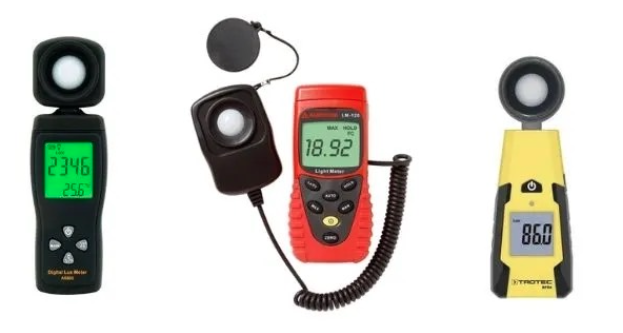
\includegraphics[height=1.7in,width=4.2in]{figuras/fig02i} 
\caption{Diferentes tipos de lux�metro}
\label{luxi}
\end{center}
\end{figure}















\chapter{Redondeo, cifras significativas y orden de magnitud}



\section{Introducci�n}
En este cap�tulo, se abordar�n una serie de conceptos fundamentales relacionados con el manejo de datos num�ricos obtenidos en el contexto del laboratorio. Cuando se efect�an c�lculos con tales datos, surge la necesidad de redondear n�meros para obtener un valor aproximado que sea conciso y evite la representaci�n enga�osa de la precisi�n de una cifra, medida o estimaci�n en los resultados calculados. En este sentido, resulta crucial considerar los d�gitos significativos de un n�mero que sean confiables y esenciales para expresar con precisi�n la magnitud en cuesti�n.



\section{Redondeo}
En muchos casos, los valores obtenidos de experimentos pueden ser redondeados a un n�mero espec�fico de cifras significativas, prescindiendo de uno o m�s de sus �ltimos d�gitos. Por ejemplo, se puede reemplazar 23,4476 por 23,45, la fracci�n 312/937 por 1/3 o la expresi�n $\sqrt{2}$ por 1,414.

El proceso de redondeo suele seguir una regla general: cuando el primer d�gito que se quiere suprimir es menor que 5, el �ltimo d�gito conservado se mantiene sin cambios; por otro lado, cuando el primer d�gito a suprimir es igual o mayor a 5, se aumenta en una unidad la �ltima cifra conservada (ver ejemplos en la tabla 2.1).

 $$
\begin{aligned}
&\text { Tabla 2.1: Ejemplos de redondeo de un n�mero}\\
&\begin{array}{|c|c|c|c|c|c|c|}
\hline & \text { N�mero } & 5 \text { cifras } & 4 \text { cifras } & 3 \text { cifras } & 2 \text { cifras } & 1 \text { cifra } \\ \hline
\hline \text { a } & 3.14159  & 3.1416  & 3.142  & 3.14  & 3.1 & 3  \\
\hline \text { b } & 9.8070 \times 10^{-3} & 9.8070 \times 10^{-3} & 9.807 \times 10^{-3} & 9.81 \times 10^{-3} & 9.8 \times 10^{-3} & 1 \times 10^{-2} \\
\hline \text { c } & 0.644510 & 0.64451 & 0.6445 & 0.645 & 0.64 & 0.6 \\
\hline \text { d } & 327508 & 32751 \times 10 & 3275 \times 10^2 & 328 \times 10^3 & 33 \times 10^4 & 3 \times 10^5 \\
\hline
\end{array}
\end{aligned}
$$

Note que el redondeo no debe hacerse en forma sucesiva, sino con respecto a la cifra original. Si en el ejercicio c, se realiza un redondeo sucesivo, el resultado ser�a:
$$
0,644510 \Rightarrow 0,64451 \Rightarrow 0,6445 \Rightarrow 0,645 \Rightarrow 0,65 \Rightarrow 0,7 \text {. }
$$
Note que el n�mero 0,7 difiere m�s de 0,644510 que el n�mero 0,6. 
 
 
 
 \section{Cifras Significativas}

Las cifras significativas en el valor de una magnitud son todos los d�gitos contados desde el primero que es diferente de cero, empezando desde la izquierda, sin considerar la posici�n de la coma decimal, hasta el primer d�gito que se ve afectado por el error. Si un n�mero que representa el resultado de una medici�n, como la longitud, la presi�n o la masa, tiene m�s d�gitos que los permitidos por la resoluci�n de la medici�n, solo se consideran fiables los d�gitos que la resoluci�n permite. Estos d�gitos son los que se denominan "cifras significativas."

A continuaci�n, se presentan ejemplos en los que el d�gito dudoso, es decir, aquel que est� afectado por el error, se encuentra resaltado en negrita.

Ejemplos:

\begin{enumerate}
\item   1,23{\bf 1} m; 123,{\bf 1} cm; 123{\bf 1} mm, tienen todos 4 cifras significativas.

\item   21,0{\bf 3} g y 200,{\bf 3} cm tienen 4 cifras significativas.

\item   2,0{\bf 0} cm y 74{\bf 0} m tienen 3 cifras significativas.

\item   0,4{\bf 8} s y 0,005{\bf 2} g tienen 2 cifras significativas.

\item    $32{\bf 3}\times10^{-3}$ kg y $3,0{\bf 0}\times10^{8}$	m/s tienen 3  significativas.
\end{enumerate}

Es oportuno observar en el ejemplo 4, que los valores de las magnitudes se han descrito con dos cifras significativas y no con tres (3) y cinco (5) respectivamente, ya
que los ceros a la izquierda no se deben contar como cifras significativas.
 

\subsection{Operaciones con cifras significativas}

\subsubsection{Suma y Resta}

Cuando realizamos operaciones de suma y resta con magnitudes que tienen diferentes cantidades de cifras significativas, es necesario redondear el resultado final para que tenga el mismo n�mero de cifras decimales que la magnitud que posea menos cifras decimales.

Por ejemplo, consideremos la suma y resta de masas expresadas en gramos.
\begin{table}[htp]
\begin{center}
\begin{tabular}{ccc}
 \text {1) } 25,340      & \text {2) } 58,0    & \text {3) }\, 1,6523    \\
\qquad            5,465  & \qquad  \quad  0,038  &\quad   -0,015     \\
\qquad            0,322  & \qquad  \quad \  1,0001&\quad   ---------    \\  
\qquad           ---------  & \qquad  \quad ---------   &\quad 1,6373     \\  
\qquad          31,127   &  \qquad \quad  59,0381 &                    \\ 
\end{tabular}
\end{center}
\end{table}

En los ejemplos 2 y 3 se observa que los resultados son m�s precisos que uno de los t�rminos (58,0 g y 0,015 g respectivamente). Por lo tanto, es necesario redondear el resultado al n�mero de decimales de la magnitud menos precisa. As�, las soluciones ser�n:
$$
\text{1)}\,\, 31,127 \mathrm{~g} \quad \text{2)}\,\, 59,0 \mathrm{~g} \quad\text{3)}\,\, 1,637 \mathrm{~g} 
$$

\subsubsection{Multiplicaci�n y Divisi�n}

Cuando realizamos operaciones de multiplicaci�n y divisi�n con magnitudes que tienen diferentes cantidades de cifras significativas, es necesario redondear el resultado final para que tenga el mismo n�mero de cifras significativas que el factor que posea menos cifras significativas.
\begin{enumerate}
\item $7.485 \mathrm{~m} \cdot 8.61 \mathrm{~m} = 64.4 \mathrm{~m}^2$
\item $7485 \mathrm{~m} \cdot 8.61\mathrm{~m}= 644 \times 10^2 \mathrm{~m}^2$
\item $\dfrac{0.1342}{1.54}= 0.0871$
 \end{enumerate}

\textbf{Observaci�n:} Es importante destacar que cuando se conoce el error absoluto (o el error probable) de una magnitud, es precisamente este error el que determina el n�mero de cifras significativas que debe tener la magnitud.


\section{Orden de magnitud}

El orden de magnitud de una cantidad se refiere a la potencia de diez m�s cercana a dicha cifra.

Por ejemplo,
\begin{enumerate}
\item  La masa de la tierra es $5,983 \times 10^{24}$ kg. Su orden de magnitud en el sistema SI es $10^{25}$ kg y en el sistema CGS es $10^{28}$ g.
\item	El orden de magnitud de 0,0035 es $10^{-3}$.

\item	El orden de magnitud de $800 \times 10^{-3}$ es $10^0$ cm.
\end{enumerate}

\textbf{Observaci�n:}  Si la cantidad f�sica es dimensional, su orden de magnitud tambi�n es dimensional y depende del sistema de unidades considerado, como se ejemplifica en los casos 1 y 3. El exponente de la potencia de 10 puede ser positivo, negativo o cero.

Tomemos el ejemplo 1 para ilustrar c�mo se puede determinar el orden de magnitud de una cantidad f�sica. Para ello, responderemos a la siguiente pregunta: �cu�les son las potencias de 10 consecutivas, inmediatamente menor y mayor que la cantidad f�sica considerada?
$$
{10^{24}} \mathrm{~kg}<5,983 \times 10^{24} \mathrm{~kg}<10^{25} \mathrm{~kg}
$$
�Cu�les son las diferencias respectivas?
$$
\begin{aligned}
& 5,983 \times 10^{24} \mathrm{~kg}-10^{24} \mathrm{~kg}=4,983 \times 10^{24} \mathrm{kg} \\
& 10^{25} \mathrm{~kg}-5,983 \times 10^{24} \mathrm{~kg}=4,017 \times 10^{24} \mathrm{~kg} \\
&
\end{aligned}
$$
La menor diferencia que es ($4,017 \times 10^{24}$) implica mayor proximidad, luego $10^{25}$ es la potencia que se aproxima m�s a $5,983 \times 10^{24}$.

\section{Ejercicios}
\begin{enumerate}
\item Determinar el n�mero de cifras significativas y el orden de magnitud de las siguientes magnitudes f�sicas.
\begin{enumerate}
\item Radio de la tierra = $6, 371 \times 10^6 \mathrm{~m}$.
\item	Volumen de la tierra =$1, 087 \times 10^{21} \mathrm{~m}^3$
\item	Aceleraci�n de gravedad=$9,80665 \mathrm{~m}/\mathrm{s}^2$
\end{enumerate}

\item Exprese el resultado de los siguientes problemas en �rdenes de magnitud
\begin{enumerate}
\item La edad del universo se cree que es $3 \times 10^{10}$ a�os, d� el resultado en segundos.
\item La velocidad de la luz en el vac�o en: $\mathrm{~m}/\mathrm{s}$,$ \mathrm{~m}/\mathrm{h}$ y en $\mathrm{~km}/\mathrm{dias}$
\item La d�nsidad del hierro en	$\mathrm{~kg}/\mathrm{m}^3$ y en  $\mathrm{~g}/\mathrm{cm}^3$
\end{enumerate}

\item Un estudiante determin� que el radio de una esfera es $R=10,00$ mm.
\begin{enumerate}
\item �Cu�nto mide su �rea?
\item�Cu�nto mide su volumen?
\item Indique el orden de magnitud para las tres magnitudes f�sicas anteriores.
\end{enumerate}

\item Exprese cada uno de los siguientes n�meros con cuatro, tres, dos y una cifra significativa:
$$
\begin{array}{|c|c|c|}
\hline 0,4536 & 98,372 & 70045,6 \\
\hline \hline 163571 & 3,13100 & 26,39 \\
\hline \hline 0,45330 & 0,00332998 & 20150,0 \\
\hline
\end{array}
$$
\item Calcule el valor de $L$ con las cifras significativas correspondientes:
$$
L=\frac{k^2}{a} +a
$$
Donde $k = 14.3$ cm y $a= 853$ mm.

\end{enumerate}




\chapter{Teor�a de Errores}

\section{Introducci�n}

Esta secci�n se centrar� en la teor�a de errores en el contexto de las mediciones experimentales. Se explorar�n los tipos de errores, incluyendo errores sistem�ticos y aleatorios, y se discutir�n estrategias para minimizar y cuantificar estos errores. Adem�s, se introducir�n m�todos para calcular incertidumbres.

Cuando se realiza la medida de una magnitud f�sica un cierto numero de veces, se observa que no todos los valores son iguales entre si y l�gicamente nos preguntamos �Cu�l es el valor correcto? �Por qu� los valores obtenidos son diferentes?

Antes de contestar estas preguntas, debemos decir que ninguna medici�n  puede dar un valor absolutamente exacto de una cantidad f�sica. Es por ello que, cuando hablamos del valor ``verdadero'' de una magnitud f�sica o valor exacto (valor que tendr�a la magnitud si no estuviese afectada de ning�n tipo de error) debemos entenderlo como una abstracci�n.

Se puede emplear los m�todos e instrumentos t�cnicos m�s perfeccionados y de todos modos ninguna medici�n lleva a un valor exacto, sino a la posibilidad de indicar un intervalo en el cual debe estar comprendido el ``verdadero valor'' para la magnitud medida.

Por ejemplo, si se mide la longitud de un objeto con una regla graduada, se puede decir que el resultado tiene una incertidumbre de $\pm 1$ mm, y  el resultado se puede escribir como  $5,5 \pm 0,1$ cm. Pero si se utiliza un vernier, el cual permite obtener una medida con m�s precisi�n, el resultado ser�a $5,530 \pm 0,005$ cm.

\section{Exactitud, precisi�n y sensibilidad}

\begin{itemize}
\item Exactitud: se refiere al grado de concordancia entre el valor �verdadero�\footnote{Por ahora lo que entendemos como valores �verdaderos� luego los definiremos como valores medios.}  y el medido experimentalmente. Decimos que un aparato es exacto si las medidas realizadas con �l son todas muy pr�ximas al valor �verdadero�de la magnitud medida.
\item Precisi�n: tiene que ver con la concordancia entre las medidas de una misma magnitud realizadas en condiciones sensiblemente iguales, un aparato es m�s preciso cuando la diferencia entre diferentes mediciones de una misma magnitud sean muy peque�as. Notemos que la exactitud normalmente implica precisi�n, pero la afirmaci�n inversa no es cierta, ya que pueden existir aparatos muy precisos que posean poca exactitud, debido a errores sistem�ticos, como por ejemplo el �error del cero�. 

Por lo tanto, precisi�n y exactitud no son sin�nimos, la precisi�n tiene que ver con la capacidad que tiene el instrumento para tomar una medida mientras que exactitud tiene que ver con el hecho de lo cerca que pueda estar una medici�n al valor real.

\item Sensibilidad: se relaciona con el valor m�nimo de la magnitud que es capaz de medir un aparato. Cuando decimos que la sensibilidad de una balanza es de 1 mg, significa que para masas inferiores a este valor la balanza no muestra ninguna desviaci�n. Por lo general consideramos la sensibilidad de un aparato de medida como el valor de la divisi�n m�s peque�a de la escala de medida. 

As� como es importante no confundir precisi�n con exactitud, tambi�n es importante no confundir precisi�n y sensibilidad.
\end{itemize}

\section{Tipos de errores en las mediciones}

\subsection{Errores sistem�ticos}
Son aquellos errores que afectan los resultados en una misma direcci�n y pueden ser causados por:
\begin{enumerate}
\item Defectos y errores de calibraci�n de los instrumentos. Por ejemplo, si el cero del tambor de un tornillo microm�trico no coincide con el cero de la escala fija, se introducir� una desviaci�n que ser� igual para todas las medidas realizadas. Esto se puede remediar recalibrando el instrumento.
\item El observador (errores personales). Puede introducir errores por efectos de paralaje. Se deben evitar estando consciente de las causas que los originan.
\item Variaci�n de las condiciones ambientales. En este caso el observador no tiene control.
\item El m�todo empleado.  En este caso, los errores solo se hacen evidentes, si se cambia el m�todo.
\end{enumerate}
Para tratar estos errores de manera segura es necesario poder controlar el correcto funcionamiento de los equipos de medida.

\subsection{Errores casuales o accidentales}

Son aquellos errores producto de una contribuci�n de fuentes incontrolables que van desplazando aleatoriamente el valor medido por encima y por debajo de su valor real, esto hace que las medidas den resultados diferentes. Se les conoce tambi�n como errores aleatorios o estad�sticos.  Los errores casuales, a diferencia de los errores sistem�ticos, son inevitables y est�n presentes en todo experimento porque son una consecuencia de  m�ltiples fluctuaciones incontrolables e independientes de los factores que intervienen en la realizaci�n de una medici�n.

Pueden ser causados por:
\begin{enumerate}
\item Condiciones ambientales fluctuantes, tales como: temperatura, presi�n variaciones de voltaje en la linea.
\item Oscilaciones de los mecanismos propios del instrumento de medida.
\item El observador.
\item Factores que puedan introducir errores que contribuyen al error total en los que podemos mencionar los siguiente: vibraciones mec�nicas, se�ales par�sitas en instrumentos electr�nicos, defectos de f�brica, etc.
\end{enumerate}

Como se trata de errores al azar, es casi imposible decidir si el promedio de las medidas se aleja hacia arriba o hacia abajo del valor exacto, por esto dicho error se expresa acompa�ado del signo de indeterminaci�n $\pm$ . En el caso de errores sistem�ticos se puede al menos en principio, determinar su signo.

\subsection{Errores de precisi�n}

Los equipos de medici�n poseen escalas o d�gitos y la divisi�n m�s peque�a de la escala o el �ltimo d�gito determina la m�nima diferencia de magnitud que puede apreciar el equipo, es decir: su resoluci�n.

Una cinta m�trica se encuentra dividida en cent�metros y mil�metros, por lo tanto, las medidas que se realicen con la cinta nos permitir� conocer la longitud de un objeto con un error aproximado de 1 mm. En el caso de que queramos disminuir el error de la medida debemos utilizar un dispositivo de medici�n que tenga una mayor resoluci�n.

Este tipo de error se le conoce como el error de precisi�n y se debe a la resoluci�n, sensibilidad, del aparato de medida. Suele designarse con $\varepsilon_p$

\section{La escritura de los resultados de una medici�n}

Al medir una magnitud $x$ y conocer el error involucrado en la medici�n $\Delta x$ debemos expresar la medida de la siguiente manera
\begin{equation}
x=x_0 \pm \Delta x \quad \text { [unidades] }
\end{equation}
\begin{itemize}
\item $x_0$ es el valor de la medida
\item  $\Delta x$ es la incertidumbre o el error de la medida
\end{itemize}
Nota: la medida y el error se deben dar en las mismas unidades.

Por ejemplo, con una cinta m�trica se ha medido la altura de una persona. El resultado obtenido es de $1.68 \mathrm{~m}$, y el error cometido es $1 \mathrm{~cm}$. La forma correcta de expresar el resultado de la medida es:
$$
\text { altura }=1,68 \pm 0,01 \mathrm{~m}\,.
$$

\subsection{Error absoluto y error relativo}

Cuando medimos una magnitud f�sica cuyo valor ``verdadero'' es $x_0$, lo que obtenemos por el proceso de medici�n es un  valor  $x$ de la medida, el {\bf error absoluto} de dicha medida es la siguiente diferencia
\begin{equation}
\Delta {x}=|{x}-{x}_0| \,,
\end{equation}
en donde suponemos que $\Delta x \ll\left|x_0\right|$.

El error absoluto nos da una medida de la desviaci�n, en t�rminos absolutos, respecto al valor ``verdadero". 

Conocido el el error absoluto podemos calcular el {\bf error relativo} de dicha medida: 
\begin{equation}
\varepsilon=\frac{\Delta x}{x_0},
\end{equation}
de manera que en forma porcentual se puede expresar como $\varepsilon \times 100 \%$.

Cuando vayamos a escribir el resultado de una medici�n para una magnitud M de debe indicar el grado de incertidumbre de la manera siguiente
\begin{equation}
\mathrm{M}=x \pm \Delta x \quad \text { [unidades] } \,.
\end{equation}

Es muy com�n escribir el error absoluto con solo una cifra significativa, al menos que se indique lo contrario. Si el error se ha obtenido con m�s de una cifra, se deber� a proceder a suprimir las posteriores por el m�todo del redondeo.  El valor de la magnitud debe tener s�lo las cifras necesarias para que su �ltima cifra significativa sea del mismo orden decimal que la �ltima del error absoluto, tambi�n llamada cifra de acotamiento.

Escribir el error con una o dos cifras significativas es una decisi�n un poco arbitraria, y depender� del error introducido. Por ejemplo, si tenemos un error de 0,89 m y lo redondeamos a 0,9, la diferencia introducida es ligeramente superior al 1 \%, valor que podr�a justificar el redondeo y expresar el error de una manera m�s sencilla; pero si un error de 1,4 m lo redondeamos a 1 m, la diferencia es cercana a un 40 \%, algo dif�cilmente justificable. 

En la siguiente tabla mostramos algunos ejemplos de medidas redondeando a una cifra significativa el error absoluto
$$
\begin{array}{|c|c|}
\hline \text { Incorrecto } & \text { Correcto } \\ \hline
\hline 3,319 \pm 0,123 & 3,3 \pm 0,1 \\
\hline 6,5 \pm 0,09 & 6,50 \pm 0,09 \\
\hline 428,364 \pm 0,28 & 428,4 \pm 0,3 \\
\hline 0,01695 \pm 0,0056 & 0,017 \pm 0,006 \\
\hline 46276 \pm 1563 & (46 \pm 2) \times10^3 \\
\hline
\end{array}
$$


\section{Mediciones directas}

Cuando hacemos una medida directamente de un aparato de medici�n decimos que hacemos una medida directa. En lo que sigue vamos a estudiar el tratamiento de los errores suponiendo  que las medidas est�n libres de errores sistem�ticos. 

\subsection{C�lculo de los errores con una sola medida}

En el caso de realizar una sola medida $x$ de una magnitud, el error cometido vendr�  dado �nicamente por el error de precisi�n del aparato utilizado, es decir,  $ \varepsilon_p= \Delta x$ . 

Pero es necesario diferenciar si la medida la hacemos con un aparato anal�gico o digital.

\begin{itemize}
\item Anal�gico: el error de precisi�n se toma como la mitad de la divisi�n mas peque�a  que puede medir el instrumento, es decir, la mitad de su sensibilidad.
\begin{equation}
\varepsilon_p= \frac{\text{divisi�n m�s peque�a}}{2} 
\end{equation}

Por ejemplo, supongamos que un amper�metro anal�gico tiene una escala de lectura que aprecia valores hasta d�cimas de amperio (sensibilidad: S=0,1 A) y, al hacer una medida, la aguja se queda entre 0,6 A y 0,7 A. En ese caso, se podr� tomar como valor experimental de la corriente $I = 0,65$ A y como error absoluto $\varepsilon_p=(0,1)/2 = 0,05$ A. Se dir� que la intensidad de corriente es de $0,65 \pm 0,05$ A.

Para una regla  dividida mil�metros el error de precisi�n en mil�metros es
de $ \varepsilon_p$ = 0,5 mm.

\item Digital: el error de precisi�n es la m�nima magnitud que puede medir el instrumento.
\begin{equation}
 \varepsilon_p = \text{m�nima magnitud medible}
\end{equation}

Por ejemplo, supongamos que un cron�metro digital que mide hasta mil�simas de segundo (sensibilidad: S = 1 ms) nos permite medir el per�odo de oscilaci�n de un p�ndulo en $T = 882$ ms. El error absoluto en este caso es $\varepsilon_p=1$ ms. Por lo tanto, el resultado se debe escribir como: $T=882 \pm 1$ ms.

\end{itemize}

\subsection{C�lculo de los errores en una serie de medidas}

En esta secci�n nos referimos solo a los errores casuales, cuyo c�lculo necesita del uso de la teor�a estad�stica. Esta teor�a es v�lida cuando el n�mero de medidas que ser realiza es grande.

En el laboratorio elemental se considera que el n�mero de medidas es grande, cuando $n \geq 25$. Pero no debe considerarse a este n�mero como un valor fijo. Para otros autores, la separaci�n entre un n�mero grande y uno peque�o de medidas  puede variar.

Hemos dicho que cuando se realiza una serie de medidas de una magnitud lo m�s probable es que ellas sean diferentes, entonces uno se pregunta �cu�l es la mejor medida?

\subsubsection{C�lculo de errores en un n�mero peque�o de medidas}

Para contestar estas preguntas se acostumbra utilizar algunas definiciones necesarias. 

\paragraph{Valor medio aritm�tico:} se define como el cociente entre la suma de las medidas: $x_1, x_2, \ldots, x_n$ y el n�mero de $n$ medidas realizadas.
\begin{equation}
\bar{x}=\frac{x_1+x_2+x_3+\ldots+x_n}{n}=\frac{1}{n} \sum_{i=1}^n x_i
\end{equation}

Es decir, la media de las medidas es el valor m�s probable de la magnitud. Se puede mostrar que $\bar{x}$ es el valor m�s cercano al valor verdadero (desconocido) de una medida.

\paragraph{Error absoluto de una medida:} como mencionamos con anterioridad, se corresponde al valor absoluto de la diferencia del valor medio respecto a cada medida.
\begin{equation}
\Delta x_i=\left|\bar{x}-x_i\right|
\label{errabs}
\end{equation}

\paragraph{Error medio absoluto de una serie de medidas:} se define como el valor medio aritm�tico de los errores absolutos de cada medida.
\begin{equation}
\overline{\Delta x}=\frac{\Delta x_1+\Delta x_2+\Delta x_3+\ldots+\Delta x_n}{n}=\frac{1}{n} \sum_{i=1}^n \Delta x_i \,.
\label{errmedabs}
\end{equation}

\paragraph{Error relativo de una serie de medidas:} es dado por el cociente entre el error medio absoluto y el valor medio aritm�tico de las medidas.
\begin{equation}
\varepsilon_x=\frac{\overline{\Delta x}}{\bar{x}} \,.
\label{errel}
\end{equation}

\paragraph{Error porcentual:} se define como el producto del error relativo por 100
\begin{equation}
\varepsilon_{\%}=\varepsilon_x \times 100 \,.
\label{errpor}
\end{equation}

\paragraph{Dispersi�n $D$:} la diferencia entre los valores extremos de las medidas:
\begin{equation}
D=x_{\text {max}}-x_{\text {min}} \,.
\label{disper}
\end{equation}

\paragraph{Dispersi�n porcentual $D_{\%}$:} definido por
\begin{equation}
D_{\%}= \frac{D}{\bar{x}} \cdot 100  
\label{disperpor}
\end{equation}



\paragraph{Ejemplo 1.} Para ilustrar lo descrito antes, realizaremos el siguiente ejercicio:

Se quiere determinar el volumen de un cilindro y por lo tanto es necesario medir la altura y el di�metro del mismo. La medida de la altura se hizo una vez con una cinta m�trica, mientras que la del di�metro se realiz� cinco veces con un vernier de apreciaci�n $0,005 \mathrm{~cm}$.
$$
\text { altura }=h=(10,2 \pm 0,1) \mathrm{cm}
$$

$$
\begin{array}{|l|l|l|l|l|l|}
\hline d=\text { di�metro }(\mathrm{cm}) & 1,780 & 1,780 & 1,780 & 1,790 & 1,790 \\
\hline
\end{array}
$$

El di�metro promedio es:
$$
\bar{d}=\frac{1,780+1,780+1,780+1,790+1,790}{5}=1,784 \mathrm{~cm}
$$
En este caso la dispersi�n es:
$$
D=1,790-1,780 = 0,01 \,\Rightarrow \, D_{\%}= \frac{0,01}{1,784} \cdot 100  = 0,6 \%
$$

Los errores absolutos para cada medida del di�metro son los siguientes:
$$
\begin{aligned}
& \Delta d_1=|1,784-1,780|=0,004 \mathrm{~cm} \\
& \Delta d_2=|1,784-1,780|=0,004 \mathrm{~cm} \\
& \Delta d_3=|1,784-1,780|=0,004 \mathrm{~cm} \\
& \Delta d_4=|1,784-1,790|=0,006 \mathrm{~cm} \\
& \Delta d_5=|1,784-1,790|=0,006 \mathrm{~cm}
\end{aligned}
$$
El error absoluto del di�metro:
$$
\overline{\Delta d}=\frac{0,004 \mathrm{~cm}+0,004 \mathrm{~cm}+0,004 \mathrm{~cm}+0,006 \mathrm{~cm}+0,006 \mathrm{~cm}}{5}=0,005 \mathrm{~cm}
$$
El error relativo del di�metro:
$$
\varepsilon_d=\frac{\overline{\Delta d}}{\bar{d}}=\frac{0,005 \mathrm{~cm}}{1,784 \mathrm{~cm}}=0,0028 .
$$
El error porcentual para el di�metro:
$$
\varepsilon_{\%}=\varepsilon_d \times 100=0,0028 \times 100=0,28 \%
$$
El error relativo para la altura:
$$
\varepsilon_h=\frac{\Delta h}{h}=\frac{0,1 \mathrm{~cm}}{10,2 \mathrm{~cm}}=0,01 .
$$
El error porcentual para la altura:
$$
\varepsilon_{\%}=\varepsilon_h \times 100=0,01 \times 100=1 \% .
$$

Por lo tanto:
$$
h=(10,2 \pm 0,1) \mathrm{~cm} \quad y \quad d= (1,784 \pm 0,005)\mathrm{~cm}
$$

Vamos a reproducir el ejemplo anterior en Python. Primero que todo debemos incorprar las librerias {\bf numpy} y {\bf matplotlib}

\begin{lstlisting}[language=Python]
from numpy import *
import matplotlib.pyplot as plt
\end{lstlisting}
   
Luego introducimos los datos como un arreglo
\begin{lstlisting}[language=Python]    
d = array([1.780, 1.780, 1.780, 1.790, 1.790])
print('Num de datos:',         len(d)  )
print('promedio:',             mean(d), 'cm' )
print('suma:',                 sum(d)  )
\end{lstlisting}
\begin{tcolorbox}[width=\textwidth,colback={ghostwhite}]    
{\small Num de datos: 5 \\
promedio: 1.784 cm\\
suma: 8.92
}
\end{tcolorbox} 

Podemos calcular la dispersi�n de la siguiente manera
\begin{lstlisting}[language=Python]    
# Valores m�ximo y m�nimos del conjunto de datos
print('valor m�ximo:',  amax(d))
print('valor m�nimo:',  amin(d))
print('dispersi�n:',   (amax(d)-amin(d)).round(2))
print('dispersi�n porcentual:', ((amax(d)-amin(d))/mean(d)*100).round(1),'%')
\end{lstlisting}
\begin{tcolorbox}[width=\textwidth,colback={ghostwhite}]   
{\small valor m�ximo: 1.79 \\
valor m�nimo: 1.78 \\
dispersi�n: 0.01\\
dispersi�n porcentual: 0.6 $\%$
}
\end{tcolorbox} 

Para el error absoluto del di�metro
\begin{lstlisting}[language=Python]    
Delta_d=(sum(abs(mean(d)-d))/len(d)).round(3)
Delta_d
\end{lstlisting}
\begin{tcolorbox}[width=\textwidth,colback={ghostwhite}] 
{\small 
0.005
}
\end{tcolorbox} 

Para el error relativo del di�metro
\begin{lstlisting}[language=Python]    
err_d=(Delta_d/mean(d)) # error relativo 
err_dp=(e_d*100)    # error porcentual

print('error relativo:', err_d.round(4))
print('error porcentual:', err_dp.round(2),'%')
\end{lstlisting}
\begin{tcolorbox}[width=\textwidth,colback={ghostwhite}]  
{\small error relativo: 0.0028 \\
error porcentual: 0.28 \%
}
\end{tcolorbox} 

\subsubsection{C�lculo de errores en un n�mero grande de medidas}

Supongamos que, un estudiante necesita conocer el di�metro de un tubo de vidrio, para lo cual realiza  25 medidas, Tabla \ref{diametros}. El instrumento utilizado fue un tornillo microm�trico de apreciaci�n $0,01 \mathrm{~mm}$.
\begin{table}[h]
\begin{center}
\begin{tabular}{|c|c|c|c|c|c|}
\hline$N^{\circ}$ de la medida & $\mathrm{d}(\mathrm{mm})$ & $N^{\circ}$ de la medida & $\mathrm{d}(\mathrm{mm})$ & $N^{\circ}$ de la medida & $\mathrm{d}(\mathrm{mm})$ \\
\hline \hline 1 & 15,12 & 10 & 15,14 & 19 & 15,14 \\
\hline 2 & 15,10 & 11 & 15,15 & 20 & 15,13 \\
\hline 3 & 15,15 & 12 & 15,14 & 21 & 15,15 \\
\hline 4 & 15,17 & 13 & 15,13 & 22 & 15,13 \\
\hline 5 & 15,14 & 14 & 15,14 & 23 & 15,11 \\
\hline 6 & 15,16 & 15 & 15,13 & 24 & 15,13 \\
\hline 7 & 15,14 & 16 & 15,13 & 25 & 15,15 \\
\hline 8 & 15,12 & 17 & 15,14 & & \\
\hline 9 & 15,12 & 18 & 15,14 & & \\
\hline
\end{tabular}
\end{center}
\caption{Medidas del di�metro $d$ de un tubo}
\label{diametros}
\end{table}

�C�mo presentar estas medidas gr�ficamente? Una manera es por me�dio de un histograma, el cual no es m�s que un gr�fico del n�mero de veces que ocurre una medida (frecuencia) como funci�n del valor de �sta.

El histograma se construye de la forma siguiente: Se divide el conjunto de valores medidos en intervalos iguales y se cuenta el n�mero de veces que ocurre el valor de la medici�n en cada intervalo. El ancho de cada intervalo es arbitrario y generalmente se escoge el m�s conveniente. 

Con los valores de la tabla anterior \ref{diametros} y escogiendo como el ancho del intervalo en  0,01 mm, las frecuencias de las medidas se muestran en la tabla \ref{histo1}. 

\begin{table}[h]
\begin{center}
\begin{tabular}{|c|c|}
\hline Intervalo $(\mathrm{mm})$ & Frecuencia \\
\hline \hline \hline $15,095-15,105$ & 1 \\
\hline $15,105-15,115$ & 1 \\
\hline $15,115-15,125$ & 3 \\
\hline $15,125-15,135$ & 6 \\
\hline $15,135-15,145$ & 8 \\
\hline $15,145-15,155$ & 4 \\
\hline $15,155-15,165$ & 1 \\
\hline $15,165-15,175$ & 1 \\
\hline
\end{tabular}
\end{center}
\caption{Frecuencias de las medidas de la tabla \ref{diametros}}
\label{histo1}
\end{table}

Para hacer un histograma podemos volver al Pyhton
\begin{lstlisting}[language=Python]    
d = array([15.12, 15.10, 15.15, 15.17, 15.14, 15.16, 15.14, 15.12, 
           15.12, 15.14, 15.15, 15.14, 15.13, 15.14, 15.13, 15.13, 
           15.14, 15.14, 15.14, 15.13, 15.15, 15.13, 15.11, 15.13, 
           15.15])
plt.hist(d,edgecolor = "white", bins=8)
plt.xlabel('Di�metros')
plt.ylabel('Frecuencia')
plt.title("histograma")
plt.show()
\end{lstlisting}
\begin{figure}[h]
\begin{center}
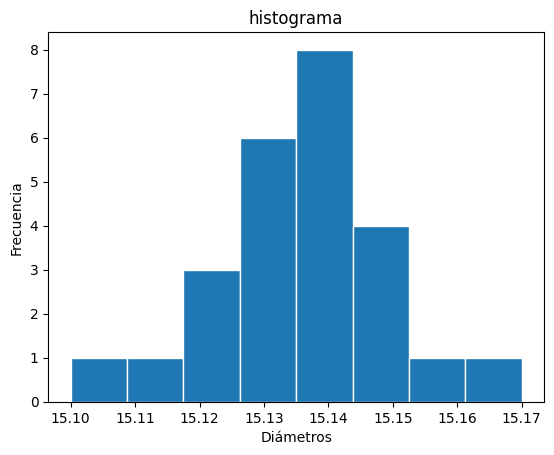
\includegraphics[height=2.5in,width=3.6in]{figuras/fig03}  
\caption{Histograma para los datos de la tabla \ref{diametros}.}
\label{gauss2}
\end{center}
\end{figure}

Si se efectuaran otras 25 mediciones, el histograma respectivo ser�a probablemen�te diferente al mostrado en \ref{gauss2}, y si se continuase haciendo medidas del di�metro hasta un n�mero $n$ muy grande y se realizara un nuevo histograma de ellas, tomando los intervalos m�s peque�os, se obtendr�a una curva continua, llamada gaussiana o curva de Gauss, ver gr�fica \ref{gauss3}. De la curva de Gauss podemos extraer la informaci�n, que nos permite decidir que tan confiables son los valores obtenidos en las medidas realizadas. 
\begin{figure}[h]
\begin{center}
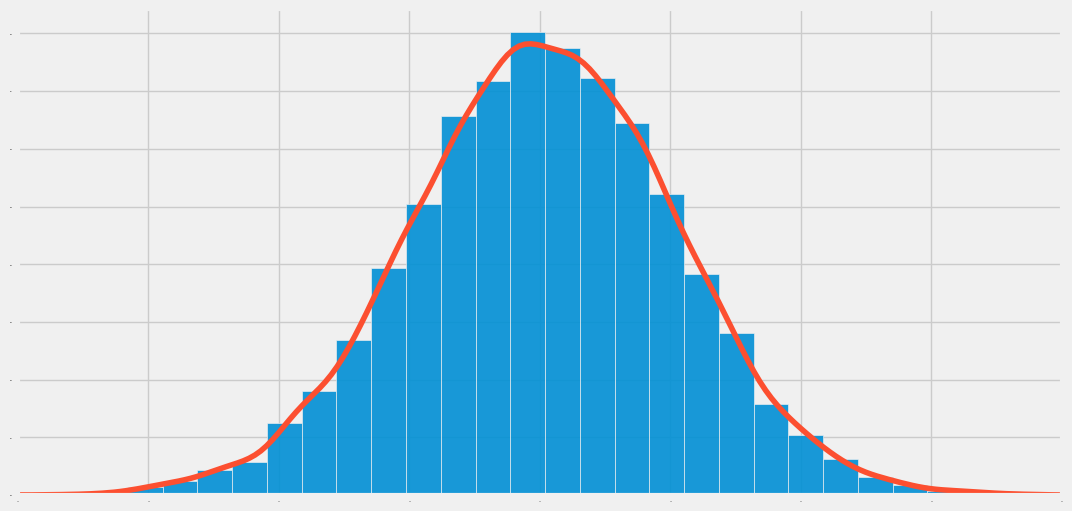
\includegraphics[height=2.5in,width=3.6in]{figuras/fig04}  
\caption{Curva de Gauss para un n�mero $n$ muy grande de medidas.}
\label{gauss3}
\end{center}
\end{figure}

Adem�s del valor medio aritm�tico $\bar{x}$ tambi�n podemos definir:
\paragraph{Desviaci�n de cada medida respecto al valor medio:} 
corresponde a la diferencia entre el valor medio y cada medida y se denota por $\Delta x_i$.
\begin{equation}
\Delta x_i=\bar{x}-x_i
\end{equation}
Las desviaciones pueden ser positivas o negativas, lo cual nos se�ala que las medidas caen a uno u otro lado del valor medio.

\paragraph{La varianza:}  se calcula tomando la desviaci�n de cada medida respecto al valor medio pero elevando al cuadrado esas diferencias, sumando esos cuadrados y luego dividiendo por el n�mero total de observaciones $n$:
\begin{equation}
\sigma^2=\frac{1}{n} \sum_{i=1}^n\left(x_i-\bar{x}\right)^2
\label{varianza}
\end{equation}

\paragraph{Desviaci�n est�ndar:} es una medida de dispersi�n que indica cu�nto var�an los valores de un conjunto de datos alrededor de su media. Es la ra�z cuadrada positiva de la varianza. Se calcula de la siguiente manera:
\begin{equation}
\sigma =\sqrt{\sigma^2}=\sqrt{\frac{1}{n} \sum_{i=1}^n\left(x_i-\bar{x}\right)^2}
\label{desest1}
\end{equation}

Dependiendo del contexto y del prop�sito del c�lculo, cuando se trabaja con poblaciones enteras o con una muestra de esa poblaci�n podemos definir la varianza y desviaci�n est�ndar muestral. 

La cantidad
\begin{equation}
s=\sqrt{\frac{\sum_{i=1}^n\left(\bar{x}-x_i\right)^2}{n-1}}
\label{des1}
\end{equation}
se conoce como la f�rmula de Bessel y se utiliza cuando la muestra es una muestra aleatoria simple de la poblaci�n y se quiere estimar la varianza de la poblaci�n a partir de la muestra.


La curva de Gauss dibujada en la figura \ref{gauss2}, ayuda a visualizar las definiciones dadas para el valor medio y la desviaci�n est�ndar.
\begin{figure}[h]
\begin{center}
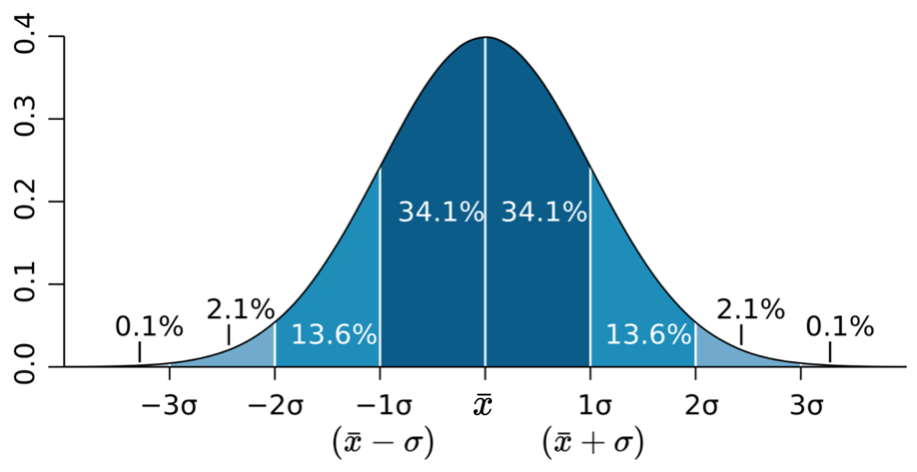
\includegraphics[height=2.1in,width=3.6in]{figuras/fig05}  
\caption{Curva de distribuci�n de Gauss mostrando la posici�n de $\bar{x}$ y $\sigma$}
\label{gauss4}
\end{center}
\end{figure}

Podemos notar que los valores de las mediciones tienden a agruparse alrededor de un punto central: la media. La representaci�n de los datos es sim�trica a ambos lados de la media y las desviaciones est�ndares quedan situadas a igual distancia unas de otras. 

Notemos tambi�n que la proporci�n de las medidas  situada entre la media y las desviaciones es una constante, por ejemplo: $\bar{x} \pm 1 \sigma$ cubre el 68,3 \% de las mediciones. Mientras que $\bar{x} \pm 3 \sigma$ cubre el 99,7 \%. 

\paragraph{Error probable $\left(\varepsilon_p\right)$}

Se define como la desviaci�n respecto al valor medio, que divide la mitad derecha (o izquierda) del �rea bajo la curva de Gauss en dos partes iguales. Por lo tanto, la probabilidad de observar una desviaci�n dentro del intervalo $\left(\bar{x}-\varepsilon_p\right)$ y $\left(\bar{x}+\varepsilon_p\right)$ es $\frac{1}{2}$, ver la figura \ref{gauss3}.
\begin{figure}[h]
\begin{center}
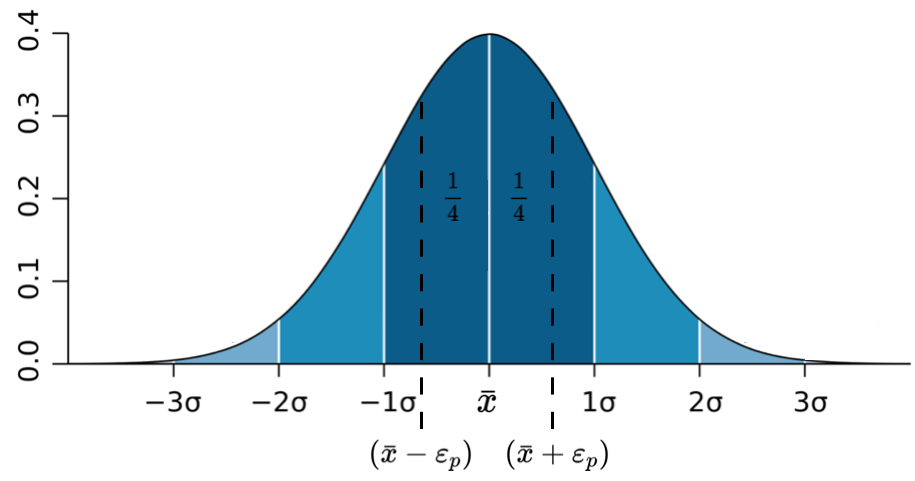
\includegraphics[height=2.1in,width=3.6in]{figuras/fig06}  
\caption{Curva de distribuci�n de Gauss mostrando la posici�n de $\bar{x}$ y $\sigma$}
\label{gauss5}
\end{center}
\end{figure}

Esto puede interpretarse diciendo que hay un $50 \%$ de probabilidad de que el valor verdadero se encuentre en ese intervalo. Para una distribuci�n de Gauss, el error probable $\left(\varepsilon_p\right)$ est� dado por:
\begin{equation}
\varepsilon_p=0,674 \sigma
\end{equation}

El estudiante debe expresar en este caso, el resultado de una serie grande de medidas como:
\begin{equation}
x=\left(\bar{x} \pm \varepsilon_p\right) \quad \text {[unidades]} \,.
\end{equation}

La teor�a estad�stica dice que de todas las medidas el:
\begin{itemize}
\item  $38,3 \%$ est�n comprendidas en el intervalo de $\bar{x}-\frac{\sigma}{2}$ hasta $\bar{x}+\frac{\sigma}{2}$.
\item  $50,0 \%$ est�n comprendidas en el intervalo de $\bar{x}-\varepsilon_p$ hasta $\bar{x}+\varepsilon_p$.
\item $68,3 \%$ est�n comprendidas en el intervalo de $\bar{x}-\sigma$ hasta $\bar{x}+\sigma$.
\item $82,2 \%$ est�n comprendidas en el intervalo de $\bar{x}-2 \varepsilon_p$ hasta $\bar{x}+2 \varepsilon_p$.
\item 95,45\% est�n comprendidas en el intervalo de $\bar{x}-2 \sigma$ hasta $\bar{x}+2 \sigma$.
\item 95,69\% est�n comprendidas en el intervalo de $\bar{x}-3 \varepsilon_p$ hasta $\bar{x}+3 \varepsilon_p$.
\item $99,73 \%$ est�n comprendidas en el intervalo de $\bar{x}-3 \sigma$ hasta $\bar{x}+3 \sigma$.
\end{itemize}

\paragraph{Ejemplo 2.} Consideremos el siguiente conjunto de medidas que se corresponden a 25 medidas para el di�metro de un tubo, Tabla \ref{diametros2}. Para ese conjunto de valores tenemos:
\begin{table}[h]
\begin{center}
\begin{tabular}{|c|c|c|c|}
\hline   &  &  &  \\
 $\mathrm{N}^{\circ}$ \text {de medida} & $d(\mathrm{mm}$) & ($\bar{d}-d$) $\mathrm{~mm}$ & ($\Delta d)^2$ mm$^2$ \\
\hline \hline 1 & 15,12 & 0,016 & 0,0003 \\
\hline 2 & 15,10 & 0,036 & 0,0013 \\
\hline 3 & 15,15 & -0,014 & 0,0002 \\
\hline 4 & 15,17 & -0,034 & 0,0011 \\
\hline 5 & 15,14 & -0,004 & 0,00002 \\
\hline 6 & 15,16 & -0,024 & 0,0006 \\
\hline 7 & 15,14 & -0,004 & 0,0002 \\
\hline 8 & 15,12 & 0,016 & 0,0003 \\
\hline 9 & 15,12 & 0,016 & 0,0003 \\
\hline 10 & 15,14 & -0,004 & 0,00002 \\
\hline 11 & 15,15 & -0,014 & 0,0002 \\
\hline 12 & 15,14 & -0,004 & 0,00002 \\
\hline 13 & 15,13 & 0,006 & 0,00004 \\
\hline 14 & 15,14 & -0,004 & 0,00002 \\
\hline 15 & 15,13 & 0,006 & 0,00004 \\
\hline 16 & 15,13 & 0,006 & 0,00004 \\
\hline 17 & 15,14 & -0,004 & 0,00002 \\
\hline 18 & 15,14 & -0,004 & 0,00002 \\
\hline 19 & 15,14 & -0,004 & 0,00002 \\
\hline 20 & 15,13 & 0,006 & 0,00004 \\
\hline 21 & 15,15 & -0,014 & 0,0002 \\
\hline 22 & 15,13 & 0,006 & 0,00004 \\
\hline 23 & 15,15 & -0,014 & 0,0002 \\
\hline 24 & 15,11 & 0,026 & 0,0007 \\
\hline 25 & 15,13 & 0,006 & 0,00004 \\
\hline \text { Suma } & $\mathbf{3 7 8 , 4 0}$ & & $\mathbf{0 , 0 0 5 8}$ \\
\hline \text { Promedio } &$ \mathbf{1 5 , 1 3 6}$ & & \\
\hline
\end{tabular}
\end{center}
\caption{Medidas para di�metro $d$ de un tubo}
\label{diametros2}
\end{table}

\begin{itemize}
\item  La desviaci�n est�ndar:
$$
\sigma=\sqrt{\frac{\sum_{i=1}^n(\Delta d)^2}{n-1}}=\sqrt{\frac{0,0058 \mathrm{~mm}^2}{24}}=0,02 \mathrm{~mm} .
$$
\item  Error probable:
$$
e_p=0,674 \times \sigma=0,01 \mathrm{~mm} .
$$
\item  Error relativo:
$$
\varepsilon_d=\frac{e_p}{\bar{d}}=\frac{0,01 \mathrm{~mm}}{15,14 \mathrm{~mm}}=7 \times 10^{-4} .
$$
\item  Error porcentual:
$$
\varepsilon_{\%}=\varepsilon_d \times 100=7 \times 10^{-4} \times 100=7 \times 10^{-2}=0,07 \% .
$$
\item  Valor del di�metro:
$$
d=(15,14 \pm 0,01) \mathrm{~mm} 
$$
\end{itemize}

Con Python podemos hacer los c�lculos del Ejemplo 2, pero es bueno notar lo siguiente. Numpy tiene una funci�n para calcular la desviaci�n est�ndar que es {\bf std} que se basa en la ecuaci�n 
$$
\sigma=\sqrt{\frac{\sum_{i=1}^n(d_i -\bar{d})^2}{n}}
$$
que ser�a la desviaci�n est�ndar  no corregida de una muestra (considerada como la poblaci�n total).
\begin{lstlisting}[language=Python]    
sig=std(d)
sig
\end{lstlisting}
\begin{tcolorbox}[width=\textwidth,colback={ghostwhite}]   
{\small 
0.014966629547095968 
}
\end{tcolorbox}

Pero aqu� estaremos utilizando la ecuaci�n \ref{des1}  que tambi�n se conoce como la desviaci�n est�ndar de una muestra corregida. Esa diferencia entre $1/n$ y $1/(n-1)$ se hace cada vez m�s peque�a a medida que $n$ aumenta. Podemos definir nuestra propia desviaci�n est�ndar.
\begin{lstlisting}[language=Python]    
des = sqrt(sum((d - mean(d))**2  )/(len(d)-1))
des
\end{lstlisting}
\begin{tcolorbox}[width=\textwidth,colback={ghostwhite}]   
{\small 
0.015275252316519673
}
\end{tcolorbox}

Para el resto de los c�lculos del ejemplo 2 tenemos:
\begin{lstlisting}[language=Python]    
epr=(0.674*des)
ed=epr/mean(d)
ep=ed*100
print('promedio:', mean(d).round(2))
print('error probable:', epr.round(2))
print('error relativo:', ed.round(4))
print('error porcentual:', ep.round(2),'%')
\end{lstlisting}
\begin{tcolorbox}[width=\textwidth,colback={ghostwhite}]   
{\small 
promedio: 15.14 \\
error probable: 0.01 \\
error relativo: 0.0007 \\
error porcentual: 0.07 \%
}
\end{tcolorbox} 


\subsection{Precisi�n y exactitud de mediciones}

Volviendo al tema de la precisi�n y exactitud de las mediciones vimos que est�n relacionadas con los errores co�metidos en la obtenci�n de las mismas. La precisi�n en el valor medio es proporcional al inverso del error casual o estad�s�tico. Se obtendr� una alta precisi�n si el error (porcentual) estad�stico es peque�o y ser� baja si dicho error es grande. La exactitud ser� alta cuando los errores sistem�ticos sean peque�os y ser� baja si �stos son grandes.

En algunos casos, una alta exactitud puede implicar un error casual peque�o, pero
en general no es as�. La precisi�n y exactitud no son t�rminos intercambia�bles entre s� y los m�todos estad�sticos dan espec�ficamente una medida cuantita�tiva de la precisi�n y no de la exactitud.

Las diferencias entre exactitud y precisi�n se ilustran en la figura \ref{gauss4}. En la figura de la izquierda se observa que el valor medio difiere bastante del valor verdadero, lo cual se interpreta diciendo que las mediciones fueron de baja exactitud, la gaussiana $B$  indica una baja exactitud y una alta precisi�n.
\begin{figure}[h]
\begin{center}
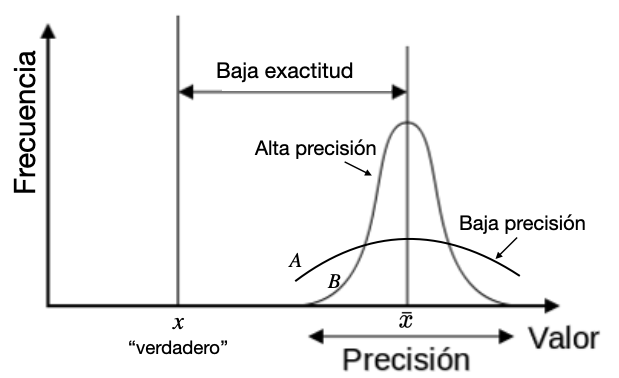
\includegraphics[height=2.1in,width=3.2in]{figuras/fig07a}  
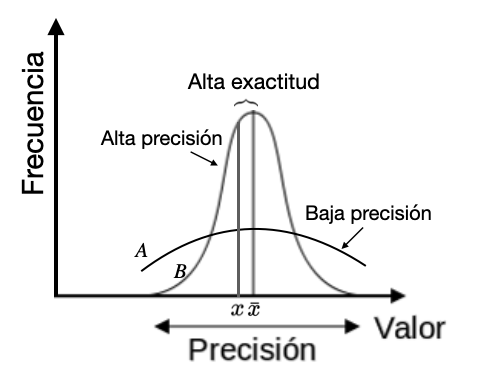
\includegraphics[height=2.1in,width=3.0in]{figuras/fig07b}  
\caption{Precisi�n y Exactitud}
\label{gauss4}
\end{center}
\end{figure}

En la misma figura pero de la derecha, en la gausiana ${B}$, el intervalo $\left(\bar{x}-\varepsilon_p, \bar{x}+\varepsilon_p\right)$ es menor que en la gaussiana $A$, por lo tanto las mediciones que corresponden a la gaussiana $B$ son de mayor precisi�n y una alta exactitud.

\subsection{Discrepancia}
Cuando tenemos dos mediciones de una misma cantidad, por ejemplo
$$
x_1=\left(x_{01} \pm \Delta x_1\right) \quad \text{y}\quad 
x_2=\left(x_{02} \pm \Delta x_2\right)
$$
decimos que tenemos una discrepancia si estas mediciones no coinciden.

Definimos la discrepancia entre dos medidas como la diferencia entre las  medidas de la misma cantidad:
$$
\text { Discrepancia}= \mathcal{D}=\left|x_{01}-x_{02}\right| 
$$

No es exactamente un error pero es una cantidad que puede ser significativa para el c�lculo de los errores.

Por ejemplo, dos estudiantes miden las siguientes temperaturas en un experimento:
$$
T_A=(2,2 \pm 0,1) \mathrm{~K} \,, \quad T_B=(2,7 \pm 0,2) \mathrm{~K} \,\, \Rightarrow \,\, 
\mathcal{D}=\left|2.2-2.7\right| = 0,5
$$
Lo anterior es igual a:
$$
2,1 \leq T_A \leq 2,3  \mathrm{~K} \quad \text{y} \quad 2,5 \leq  T_B \leq 2,9  \mathrm{~K}
$$
y se dice  que ambas mediciones son distinguibles entre s� porque los intervalos no se solapan.

Pero resulta que otros dos estudiantes miden las siguientes temperaturas
$$
T_A=(2,3 \pm 0,1) \mathrm{~K}\,, \quad T_B=(2,5 \pm 0,2) \mathrm{~K} \,\, \Rightarrow \,\, 
\mathcal{D}=\left|2.3-2.5\right| = 0,2
$$
que es equivalente  a:
$$
2,2 \leq T_A \leq 2,4  \mathrm{~K} \quad \text{y} \quad   2,3 \leq  T_B \leq 2,7  \mathrm{~K}
$$
en este caso,  la discrepancia es de 0,2  pero no es significativa porque los intervalos de las mediciones se superponen, decimos entonces que las mediciones son indistinguibles.

Podemos hablar de una discrepancia porcentual si tomamos la media de las medidas, para el primer caso el promedio de las dos medidas es: 2,45 K.
$$
\mathcal{D}_{\%}= \left|\frac{0,5}{2,45}\right| \times 100 = 20 \%
$$

Y para el segundo par de medidas el promedio es 2,4 K
$$
\mathcal{D}_{\%}= \left|\frac{0,2}{2,4}\right| \times 100 = 8 \%
$$


\section{Algoritmo para el manejo de los errores}

Podemos crear un algoritmo que nos ayude a definir los criterios que debemos utilizar a la hora de escribir los resultados de las mediciones hechas en el laboratorio. Para darle a nuestras mediciones una validez estad�stica es conveniente realizar el calculo de la dispersi�n $D$, ecuaci�n \ref{disper}, la dispersi�n porcentual \ref{disperpor} y  tener a mano la sensibilidad $S$ del aparato de medida.

Realicemos los siguientes pasos
\begin{enumerate}
\item Tomaremos $N=3$ mediciones como el valor m�nimo para nuestro algoritmo.
\begin{description}
\item[i) Si $D < S$:]  El error vendr� dado por $\Delta x= S$ y la medida es $\bar{x}_3$, por lo tanto
$$
\mathrm{M}= \bar{x}_3  \pm  S \quad \mathrm{[Unidades]} 
$$
\item [ii) Si  $D > S$ y $D_{\%} \leq 2\%$:]  El error vendr� dado por $\Delta x= S$ y la medida es $\bar{x}_3$
$$
\mathrm{M}= \bar{x}_3 \,  \pm \, S \quad \mathrm{[Unidades]} 
$$
\end{description}
donde 
$$
\bar{x}_3=\frac{1}{3}{\sum_{i=1}^3 x_i}
$$

\item Si para $N=3$ se tiene que $D > S$ pero la dispersi�n est� entre: $2\% \leq D_{\%} \leq 8\% $, entonces  realizamos m�s medidas hasta llegar a  $N=6$.  El error vendr� dada por el valor m�ximo entre $D_6/4$ y $S$, donde $D_6$ es la dispersi�n para 6 medidas, es decir:
$$
\mathrm{M}= \bar{x}_6 \,  \pm \,  \mathrm{max} \left\{D_6 /4, S \right\}  \quad \mathrm{[Unidades]} 
$$
donde
$$
\bar{x}_6=\frac{1}{6}{\sum_{i=1}^6 x_i}
$$

\item Si para $N=3$ se tiene que $D > S$ pero la dispersi�n est� entre: $8\% \leq D_{\%} \leq 15\% $, entonces  hacemos $N=15$, y el error vendr� dado por
$$
\Delta x_{15}=\sqrt{\frac{\sum_{i=1}^{15}\left(x_i-\bar{x}_{15}\right)^2}{14}}
$$
La magnitud se escribe entonces como 
$$
\mathrm{M}= \bar{x}_{15}  \pm \Delta x_{15}   \quad \mathrm{[Unidades]} 
$$
donde
$$
\bar{x}_{15}=\frac{1}{15}{\sum_{i=1}^{15} x_i}
$$

\item  Si para $N=3$ se tiene que $D > S$ per la dispersi�n es $ D_{\%} \geq 15\% $, entonces demos hacer muchas medidas $N \geq 50$, y el error vendr� dado por
$$
\Delta x_{N}=\sqrt{\frac{\sum_{i=1}^N\left(x_i-\bar{x}_N\right)^2}{N(N-1)}}
$$
La magnitud se escribe entonces como 
$$
\mathrm{M}= \bar{x}_{N}  \pm \Delta x_{N}   \quad \mathrm{[Unidades]} 
$$
donde 
$$
\bar{x}_{N}=\frac{1}{N}{\sum_{i=1}^{N} x_i} \,.
$$

Notemos que si  por ejemplo, se ha obtenido que $D > S$ y $2\% \leq D_{\%} \leq 8\% $ se necesitan  6 medidas y el valor verdadero queda establecido en la media aritm�tica de las 6 medidas y su error corresponde al m�ximo de entre la dispersi�n de las seis medidas dividido por 4 o la sensibilidad.

Por otro lado, si se realizan 15 o m�s medidas, en realidad se est� buscando que el conjunto de las mismas sea una distribuci�n gaussiana o normal, en cuyo caso, el error que se considera corresponde con el error cuadr�tico medio (ECM) o desviaci�n standard $\sigma$. 
\end{enumerate}

\paragraph{Ejemplo 3.} Con una regla graduada, en mil�metros, se mide la longitud $L$ de un tubo. El error de cada medida para este instrumento anal�gico es
$$
\varepsilon_p= \frac{1\mathrm{~mm}}{2}= 0,5 \mathrm{~mm} =S 
$$

\begin{itemize}
\item Los datos obtenidos para tres medidas son:
$$
\begin{array}{|c|c|c|c|}
\hline \hline 
L (\mathrm{mm}) &15,0 & 14,0 & 13,5 \\
\hline 
\end{array}
$$
La media:
$$
\bar{L}= \frac{15,0 + 14,0 + 13,5}{3}= \frac{42,5}{3}= 14,2 \mathrm{~mm}
$$
La dispersi�n para estos datos es de
$$
D=15,0 - 13,5 = 1,5 \,\, \Rightarrow \,\, D_{\%}= \frac{1,5}{14,2} \cdot 100  = 11 \%
$$

Estamos en el caso donde  $D > S$  y la dispersi�n porcentual resulta ser mayor al $2\%$. Debemos hacer m�s medidas

\item Agregamos tres medidas m�s para completar 6 mediciones
$$
\begin{array}{|c|c|c|c|c|c|c|}
\hline \hline 
L (\mathrm{mm}) &15,0 & 14,0 & 13,5 & 15,5&15,5 & 15,5\\
\hline 
\end{array}
$$
La media:
$$
\bar{L}=\frac{15,0 + 14,0 + 13,5+15,5+15,5 + 15,5}{6}= \frac{89,0}{6}= 14,8 \mathrm{~mm}
$$
La dispersi�n para estos datos es ahora de 
$$
D=15,5 - 13,5 = 2,0 \,\,\Rightarrow \,\, D_{\%}= \frac{2,0}{14,8} \cdot 100  = 14 \%
$$
Con $N=6$, nuevamente tenemos que $D > S$  y la dispersi�n porcentual se encuentra fuera del rango $2\% \leq D_{\%} \leq 8\% $. Debemos tomar m�s medidas. 

\item Agregamos 9 medidas m�s para completar $N=15$
$$
\begin{array}{ccc}
\hline \hline L(\mathrm{~mm}) & L(\mathrm{~mm}) & L(\mathrm{~mm}) \\\hline 
15,0 & 14,0 & 13,5 \\
15,5 & 15,5 & 15,5 \\
13,5 & 15,0 & 14,0 \\
14,0 & 14,0 & 15,5 \\
13,5 & 14,0 & 14,0 \\
\hline \hline
\end{array}
$$
La media:
$$
\bar{L}=\frac{1}{15}{\sum_{i=1}^{15} L_i} = \frac{216}{15}= 14,4 \mathrm{~mm}
$$
La dispersi�n para estos datos es ahora de 
$$
D=15,5 - 13,5 = 2,0 \,\Rightarrow \, D_{\%}= \frac{2,0}{14,4} \cdot 100  = 14 \%
$$

Con $N=15$, nuevamente tenemos que $D > S$  pero ahora la dispersi�n porcentual se encuentra dentro del rango $8\% \leq D_{\%} \leq 15\% $. Podemos parar y proceder a calcular los errores completando la  siguiente tabla
$$
\begin{array}{|c|c|c|c|}
\hline i & L_i \pm 0,5  (\mathrm{mm}) & L_i-\bar{L} (\mathrm{mm}) & \left(L_i-\bar{L}\right)^2 (\mathrm{mm}^2) \\\hline 
1 & 15,0 & 0,6 & 0,36 \\
2 & 15,5 & 1,1 & 1,21 \\
3 & 13,5 & -0,9 & 0,81 \\
4 & 14,0 & -0,4 & 0,16 \\
5 & 13,5 & -0,9 & 0,81 \\
6 & 14,0 & -0,4 & 0,16 \\
7 & 15,5 & 1,1 & 1,21 \\
8 & 15,0 & 0,6 & 0,36 \\
9 & 14,0 & -0,4 & 0,16 \\
10 & 14,0 & -0,4 & 0,16 \\
11 & 13,5 & -0,9 & 0,81 \\
12 & 15,5 & 1,1 & 1,21 \\
13 & 14,0 & -0,4 & 0,16 \\
14 & 15,5 & 1,1 & 1,21 \\
15 & 14,0 & -0,4 & 0,16 \\
\hline \sum & 216 & & 8,95 \\
\hline
\end{array}
$$

Por lo tanto:
$$
\Delta x_{15}=\sqrt{\frac{\sum_{i=1}^{15}\left(L_i-\bar{L}_{15}\right)^2}{14}}=\sqrt{\frac{8,95}{14}} =0,214  \mathrm{~mm}
$$

La longitud L del tubo  se escribe entonces como 
$$
L= 14,4  \pm 0,2  \mathrm{~mm}
$$

\end{itemize}





\section{Mediciones indirectas}
Hasta aqu� se ha analizado lo correspondiente a errores de magnitudes medidas directamente, por ejemplo: la altura de un cilindro, el di�metro de un tubo, el tiempo de ca�da de un cuerpo. Frecuentemente la magnitud de inter�s debe ser determinada a partir de otras magnitudes medidas directamente, por lo que el error en dicha magnitud debe ser obtenido a partir de los errores de las otras magnitudes.

Por ejemplo, para la determinar el volumen $V$ de un cilindro se efect�an medidas del di�metro $d$ y la altura $h$, luego el error en $V$ debe ser obtenido de los errores cometidos en las medidas de $d$ y $h$.  El procedimiento que permite obtener este error es lo que se conoce como propagaci�n de errores.

\subsection{Propagaci�n de errores}
Como indicamos anteriormente, la medida indirecta de una magnitud se alcanza por aplicaci�n de una f�rmula a un conjunto de medidas directas, (las variables independientes o los datos), que las relacionan con la magnitud del problema. Mediante dicha f�rmula se puede obtener tambi�n el error de la medida. 

\subsection{Propagaci�n de errores en casos particulares}

A continuaci�n analizaremos algunos de los casos m�s sencillos de propagaci�n de errores:

\paragraph{Suma y diferencia de magnitudes.}

Cuando una magnitud M es el resultado de la suma o resta de dos o m�s magnitudes medidas directamente, un error en dichas magnitudes traer� consigo un error en M, es decir, si $(X \pm \Delta X)$ y $(Y \pm \Delta Y)$ son dos mediciones directas, entonces 
$$
\mathrm{M}=X  \pm Y \,\, \Rightarrow \,\, \mathrm{M} \pm \Delta \mathrm{M}=(X \pm \Delta X) \pm(Y \pm \Delta Y) \,,
$$
reagrupando t�rminos resulta,
$$
\mathrm{M} \pm \Delta \mathrm{M}=(X \pm Y) \pm(\Delta X+\Delta Y)
$$
donde
$$
\Delta \mathrm{M}=\Delta X+\Delta Y
$$

El error absoluto $\Delta$M, de la suma o diferencia de magnitudes, viene dado por la suma de los errores absolutos de cada una de las magnitudes medidas directamente.

El error relativo ser�:
$$
\varepsilon_r=\frac{\Delta \mathrm{M}}{\mathrm{M}}=\frac{\Delta X+\Delta Y}{X \pm Y}
$$

\paragraph{Multiplicaci�n de magnitudes.} 
Si la magnitud M es el resultado de multiplicar dos o m�s magnitudes medidas en forma directa, el error absoluto $\Delta$M se puede obtener de la siguiente manera:
$$
\mathrm{M}  =X \cdot Y \,\, \Rightarrow \,\,  \mathrm{M} \pm \Delta\mathrm{M}  =(X \pm \Delta X) \cdot (Y \pm \Delta Y)  \,,
$$
por lo tanto
$$
\mathrm{M} \pm \Delta \mathrm{M}  =(X \cdot Y) \pm X \Delta Y \pm Y \Delta X+\Delta X \Delta Y \,.
$$

Puesto que las cantidades $\Delta X$ y $\Delta Y$ son peque�as comparadas con $X$ y $Y$, se puede despreciar el t�rmino $\Delta X \Delta Y$ y el error absoluto de $M$ ser�:
$$
\Delta \mathrm{M}=X \Delta Y+Y \Delta X \,.
$$

El error relativo:
$$
\varepsilon_r=\frac{\Delta \mathrm{M}}{\mathrm{M}}=\frac{\Delta X}{X}+\frac{\Delta Y}{Y}
$$
es decir, el error relativo de un producto de magnitudes es la suma de los errores relativos de cada una de las magnitudes medidas directamente.

\paragraph{Divisi�n de magnitudes.} 
Cuando la magnitud M es el resultado de dividir magnitudes medidas directamente, el error absoluto se puede obtener en la forma siguiente:
$$
\mathrm{M} =\frac{X}{Y} \,\, \Rightarrow \,\,  \mathrm{M} \pm \Delta \mathrm{M}  =\frac{X \pm \Delta X}{Y \mp \Delta Y} \,,
$$
por lo tanto:
$$
\mathrm{M} \pm \Delta \mathrm{M}  =\frac{X \pm \Delta X}{Y \mp \Delta Y} \cdot \frac{Y \pm \Delta Y}{Y \pm \Delta Y} =\frac{X Y \pm Y \Delta X \pm X \Delta Y+\Delta X \Delta Y}{Y^2-(\Delta Y)^2} \,.
$$

Considerando que $\Delta X$ y $\Delta Y$ son peque�os en relaci�n a $X$ y $Y$, se puede despreciar los t�rminos $\Delta X \Delta Y$ y $(\Delta Y)^2$, luego
$$
\mathrm{M} \pm \Delta\mathrm{M}=\frac{X}{Y} \pm \frac{Y \Delta X+X \Delta Y}{Y^2}\,,
$$
es decir, el error absoluto en M ser�:
$$
\Delta \mathrm{M}=\frac{Y \Delta X+X \Delta Y}{Y^2} \,,
$$
y el error relativo:
$$
\varepsilon_r=\frac{\Delta \mathrm{M}}{\mathrm{M}}=\frac{\Delta X}{X}+\frac{\Delta Y}{Y}\,.
$$

Al igual que para el producto de magnitudes, el error relativo del cociente es igual a la suma de los errores relativos de cada una de las magnitudes medidas directamente.


\paragraph{Funci�n potencial.}
Si la magnitud M es el resultado de elevar la magnitud $X$ a una potencia $n$, M$=a X^n$, donde $a$ es un valor exacto. El error relativo se puede obtener aplicando el criterio definido para el producto de magnitudes.

Ya que M se puede escribir como:
$$
\mathrm{M}=a \cdot \underbrace{X \cdot X \cdot X \ldots  X}_{n \text { veces }}
$$
su error relativo ser�:
$$
\varepsilon_r=\frac{\Delta \mathrm{M}}{\mathrm{M}}=\underbrace{\frac{\Delta X}{X}+\frac{\Delta X}{X}+\ldots+\frac{\Delta X}{X}}_{n \text { veces }}
$$
luego
$$
\varepsilon_r=\frac{\Delta \mathrm{M}}{\mathrm{M}}=n \frac{\Delta X}{X}
$$
as� que, el error absoluto ser�:
$$
\Delta \mathrm{M}=a n X^{n-1} \Delta X \,.
$$

\subsection{Propagaci�n de errores en casos generales}

En el caso en que la magnitud a determinar dependa de m�s de dos magnitudes medidas directamente y relacionadas a trav�s de diferentes operaciones matem�ticas, el c�lculo del error absoluto y del relativo se puede realizar por uno de los m�todos siguientes:

\subsubsection{M�todo del binomio}

Consideremos un caso en que la expresi�n que relaciona la magnitud M con las magnitudes $X, Y, Z$ y $T$ sea del tipo:
$$
\mathrm{M}=\frac{X^a  Y^b}{Z^c  T^d}=X^a  Y^b  Z^{-c}  T^{-d}
$$

Para la obtenci�n del error en M, supongamos que el experimento sea tan desafortunado que todos los errores influyan en el resultado en la misma direcci�n. En este caso el m�ximo error posible en $\mathrm{M}$ vendr� dado por:
$$
\begin{aligned}
\mathrm{M} \pm \Delta \mathrm{M} & =\frac{(X+\Delta X)^a (Y+\Delta Y)^b}{(Z-\Delta Z)^c  (T-\Delta T)^d}  =(X+\Delta X)^a (Y+\Delta Y) (Z-\Delta Z)^{-c} (T-\Delta T)^{-d}
\end{aligned}
$$

Esto suceder� si los valores de $X$ y $Y$ son grandes, mientras que los de $Z$ y $T$ son peque�os. La expresi�n anterior puede ser escrita en la forma siguiente:
$$
\mathrm{M} \left(1+\frac{\Delta \mathrm{M}}{\mathrm{M}}\right)=X^a Y^b Z^{-c} T^{-d} \left(1+\frac{\Delta X}{X}\right)^a\left(1+\frac{\Delta Y}{Y}\right)^b\left(1-\frac{\Delta Z}{Z}\right)^{-c}\left(1-\frac{\Delta T}{T}\right)^{-d}
$$
luego,
$$
\left(1+\frac{\Delta \mathrm{M}}{\mathrm{M}}\right)=\left(1+\frac{\Delta X}{X}\right)^a\left(1+\frac{\Delta Y}{Y}\right)^b\left(1-\frac{\Delta Z}{Z}\right)^{-c}\left(1-\frac{\Delta T}{T}\right)^{-d}
$$

Si suponemos que los errores absolutos son peque�os comparados con las magnitudes medidas, los t�rminos, $\frac{\Delta X}{X}, \frac{\Delta Y}{Y}, \frac{\Delta Z}{Z}$ y $\frac{\Delta T}{T}$ son a�n m�s peque�os, por consiguiente al desarrollar cada uno de los binomios de Newton y despreciar los t�rminos elevados al cuadrado o de potencias mayores, lo que queda es:
$$
\left(1+\frac{\Delta \mathrm{M}}{\mathrm{M}}\right) \simeq\left(1+a \frac{\Delta X}{X}\right) \left(1+b \frac{\Delta Y}{Y}\right) \left(1+c \frac{\Delta Z}{Z}\right) \left(1+d \frac{\Delta T}{T}\right)
$$

Efectuando las multiplicaciones y despreciando los productos de los t�rminos peque�os, se tiene:
\begin{equation}
\varepsilon_r=\frac{\Delta \mathrm{M}}{\mathrm{M}}=a \frac{\Delta X}{X}+b \frac{\Delta Y}{Y}+c \frac{\Delta Z}{Z}+d \frac{\Delta T}{T}
\label{binomio}
\end{equation}
es decir, el error relativo de M corresponde a la suma de los errores relativos de cada magnitud multiplicados por sus exponentes respectivos.

Si se multiplica por 100 la expresi�n anterior, se obtiene el error porcentual en $M$ como funci�n de los porcentajes de error que introducen cada una de las magnitudes:
$$
\varepsilon_{\%}=a \varepsilon_{X\%}+b \varepsilon_{Y\%}+c \varepsilon_{Z\%}+d \varepsilon_{T\%} \,.
$$

\paragraph{Ejemplo 4.} Supongamos que una magnitud M est� relacionada con las magnitudes: $X_1, X_2, Y, Z, T_1$ y $T_2$, mediante una expresi�n del tipo:
\begin{equation}
\mathrm{M}=\frac{\left(X_1+X_2\right)  Y^2}{Z\left(T_1-T_2\right)^3} \,.
\label{eme3}
\end{equation}

Para utilizar la expresi�n (\ref{binomio}), se debe llevar la expresi�n M a una forma que contenga s�lo productos y/o cocientes de magnitudes. Para lograr esto, se realiza el siguiente cambio de variables,
\begin{equation}
\begin{aligned}
X & =X_1+X_2 \\
T & =T_1-T_2
\end{aligned}
\label{camva}
\end{equation}

Como $X$ y $T$ son el resultado de una suma y una resta, respectivamente, se sabe que el error absoluto de cada una de ellas viene dado por:
$$
\begin{aligned}
\Delta X & =\Delta X_1+\Delta X_2 \\
\Delta T & =\Delta T_1+\Delta T_2
\end{aligned}
$$
Usando (\ref{camva}) M se puede expresar como:
$$
\mathrm{M}=\frac{X  Y^2}{Z  T^3}
$$
De acuerdo a la expresi�n (\ref{binomio}), el error relativo de M ser�:
$$
\varepsilon_r=\frac{\Delta \mathrm{M}}{\mathrm{M}}=\frac{\Delta X}{X}+2 \frac{\Delta Y}{Y}+\frac{\Delta Z}{Z}+3 \frac{\Delta T}{T} \,.
$$


\paragraph{Ejemplo 5.} Para calcular los errores en el volumen del cilindro estudiado anteriormente, (Ejemplo 1) se har� uso de la expresi�n (\ref{binomio}).

Con los valores medidos de $h= (10,2 \pm 0,1)$ cm y $d=(1,784 \pm 0,005)$ cm, el volumen del cilindro estar� dado por:
$$
V=\pi r^2 h=\frac{\pi d^2 h}{4}=\frac{\pi (1,784)^2  (10,2)}{4}= 25,5 \mathrm{~cm}^3 \,.
$$

El error relativo ser�:
$$
\varepsilon_r=\frac{\Delta V}{V}=2 \frac{\Delta D}{D}+\frac{\Delta h}{h}=2 \cdot (0,0028)+0,01=0,016 \,.
$$
El error porcentual,
$$
\varepsilon_{\%}=\varepsilon_r \cdot 100=0,016 \cdot 100=1,6 \simeq 2 \% \,.
$$
El error absoluto,
$$
\Delta V=0,016 \cdot V=0,4 \mathrm{~cm}^3\,,
$$
luego el valor calculado de $V$ se escribe de la siguiente manera:
$$
V=(25,5 \pm 0,4) \mathrm{cm}^3
$$

Nota: El error absoluto de la magnitud f�sica se escrib�o con una cifra significativa. Esto condiciona el n�mero de cifras significativa del valor de la magnitud.

\subsubsection{M�todo de las derivadas parciales}
Existe un m�todo alternativo al dado anteriormente para la propagaci�n de errores, el cual hace uso de las derivadas y que explicaremos a continuaci�n.

Sea una magnitud M, la cual es funci�n de las magnitudes independientes $X, Y, Z, T, \ldots$
$$
\mathrm{M}=\mathrm{M}(X, Y, Z, T, \ldots)
$$

El error en M es producido por cada uno de los errores de las magnitudes $X, Y, Z, T, \ldots$, independientemente uno de los otros. A estos errores se les llama errores parciales y la suma de ellos, considerando el caso m�s desfavorable, dar� el error en M.

El error absoluto en M estar� dado por:
\begin{equation}
\Delta \mathrm{M}=\left|\frac{\partial \mathrm{M}}{\partial X}\right||\Delta X|+\left|\frac{\partial \mathrm{M}}{\partial Y}\right||\Delta Y|+\left|\frac{\partial \mathrm{M}}{\partial Z}\right||\Delta Z|+\left|\frac{\partial \mathrm{M}}{\partial T}\right||\Delta T|+\ldots
\end{equation}
donde los t�rminos $\frac{\partial \mathrm{M}}{\partial X}, \frac{\partial \mathrm{M}}{\partial Y}, \frac{\partial \mathrm{M}}{\partial Z}, \frac{\partial \mathrm{M}}{\partial T}, \ldots$ son las derivadas de M con respecto a $X, Y, Z, T, \ldots$, respectivamente. 

Estas se determinan derivando la funci�n M con respecto a cada una de las variables en forma separada y considerando constantes las dem�s, es decir, al derivar M con respecto a $X$ se considera a las variables $Y, Z, T, \ldots$ como constantes, y as� sucesivamente cuando se deriva respecto a $Y$, � a $Z, \ldots$

El error relativo se determina como el cociente entre el error absoluto y la funci�n misma.
\begin{equation}
\varepsilon_{\mathrm{r}}=\frac{\Delta \mathrm{M}}{\mathrm{M}}=\frac{1}{\mathrm{M}(X, Y, Z, T, \ldots)}\left\{\left|\frac{\partial \mathrm{M}}{\partial X}\right||\Delta X|+\left|\frac{\partial \mathrm{M}}{\partial Y}\right||\Delta Y|+\left|\frac{\partial \mathrm{M}}{\partial Z}\right||\Delta Z|+\left|\frac{\partial \mathrm{M}}{\partial T}\right||\Delta T|+\ldots\right\}
\end{equation}

\paragraph{Ejemplo 6.}

Obtendremos el error relativo para la expresi�n (\ref{eme3}) del ejemplo 3, utilizando el m�todo de las derivadas parciales:
$$
\mathrm{M}=\frac{\left(X_1+X_2\right)  Y^2}{Z \left(T_1-T_2\right)^3}
$$
Las derivadas parciales de M respecto a cada una de las variables son las siguientes:
\begin{eqnarray*}
\frac{\partial \mathrm{M}}{\partial X_1}&=&\frac{Y^2}{Z\left(T_1-T_2\right)^3}\,, \quad 
\frac{\partial \mathrm{M}}{\partial X_2}=\frac{Y^2}{Z\left(T_1-T_2\right)^3}\,, \quad
\frac{\partial \mathrm{M}}{\partial Y}=\frac{2 Y\left(X_1+X_2\right)}{Z\left(T_1-T_2\right)^3}\,\\
\frac{\partial \mathrm{M}}{\partial Z}&=&-\frac{\left(X_1+X_2\right)Y^2}{Z^2\left(T_1-T_2\right)^3} \,,\quad  \frac{\partial \mathrm{M}}{\partial T_1}=-\frac{3\left(X_1+X_2\right) Y^2}{Z\left(T_1-T_2\right)^4} \,,\quad \frac{\partial \mathrm{M}}{\partial T_2}=\frac{3\left(X_1+X_2\right) Y^2}{Z\left(T_1-T_2\right)^4}
\end{eqnarray*}

El error absoluto ser�:
$$
\Delta \mathrm{M}=\left|\frac{\partial \mathrm{M}}{\partial X_1}\right|\left|\Delta X_1\right|+\left|\frac{\partial \mathrm{M}}{\partial X_2}\right|\left|\Delta X_2\right|+\left|\frac{\partial \mathrm{M}}{\partial Y}\right||\Delta Y|+\left|\frac{\partial \mathrm{M}}{\partial Z}\right||\Delta Z|+\left|\frac{\partial \mathrm{M}}{\partial T_1}\right|\left|\Delta T_1\right|+\left|\frac{\partial \mathrm{M}}{\partial T_2}\right|\left|\Delta T_2\right|\,.
$$
Por lo tanto
$$
\begin{aligned}
\Delta \mathrm{M} & =\frac{Y^2}{Z\left(T_1-T_2\right)^3} \Delta X_1+\frac{Y^2}{Z\left(T_1-T_2\right)^3} \Delta X_2+\frac{2 Y\left(X_1+X_2\right)}{Z\left(T_1-T_2\right)^3} \Delta Y  \\
& +\frac{\left(X_1+X_2\right) Y^2}{Z^2\left(T_1-T_2\right)^3} \Delta Z+\frac{3\left(X_1+X_2\right) Y^2}{Z\left(T_1-T_2\right)^4} \Delta T_1+\frac{3\left(X_1+X_2\right) Y^2}{Z\left(T_1-T_2\right)^4} \Delta T_2
\end{aligned}
$$
Simplificando:
$$
\begin{aligned}
\Delta \mathrm{M} & =\frac{Y^2\left(\Delta X_1+ \Delta X_2\right)}{Z\left(T_1-T_2\right)^3}  + \frac{Y\left(X_1+X_2\right)}{Z\left(T_1-T_2\right)^3} \left[{2\Delta Y}+\frac{Y\Delta Z}{Z}  \right]  \\
&+ \frac{3\left(X_1+X_2\right) Y^2 \left(\Delta T_1+ \Delta T_2\right)}{Z\left(T_1-T_2\right)^4} 
\end{aligned}
$$

El error relativo:
$$
\begin{aligned}
& \varepsilon_{\mathrm{r}}=\frac{\Delta \mathrm{M}}{\mathrm{M}}  = \frac{Z \left(T_1-T_2\right)^3}{\left(X_1+X_2\right)  Y^2} 
\left\{ \frac{Y^2\left(\Delta X_1+ \Delta X_2\right)}{Z\left(T_1-T_2\right)^3}  + \frac{Y\left(X_1+X_2\right)}{Z\left(T_1-T_2\right)^3} \left[{2\Delta Y}+\frac{Y\Delta Z}{Z}  \right]     \right. \\
& \left.+  \frac{3\left(X_1+X_2\right) Y^2 \left(\Delta T_1+ \Delta T_2\right)}{Z\left(T_1-T_2\right)^4} \right\} \\
\end{aligned}
$$
simplificamos nuevamente y finalmente  obtenemos
\begin{equation}
\frac{\Delta \mathrm{M}}{\mathrm{M}}=\frac{\Delta X_1+\Delta X_2}{X_1+X_2}+2 \frac{\Delta Y}{Y}+\frac{\Delta Z}{Z}+3 \frac{\Delta T_1+\Delta T_2}{T_1-T_2}
\end{equation}

Vemos que la expresi�n anterior para el error relativo coincide con la obtenida  por el m�todo del binomio del ejemplo 4. Se debe notar que el m�todo de las derivadas es m�s laborioso y necesita del conocimiento de las derivadas parciales. Sin embargo, este �ltimo m�todo es aplicable a cualquier expresi�n, mientras que el m�todo del binomio s�lo es valido para expresiones que contengan solamente variables independientes.

Para ilustrar esto �ltimo obtengamos el error relativo para la expresi�n:
$$
\mathrm{M}=\frac{(a+z)^2}{(b+z)^2}
$$
donde $a$ y $b$ son constantes exactas.
\begin{description}
\item[a)]  M�todo del binomio

Primero realizaremos el siguiente cambio de variables:
\begin{itemize}
\item  $A=a+z \Rightarrow \Delta A=\Delta z$
\item  $B=b+z \Rightarrow \Delta B=\Delta z$
\end{itemize}

Note que las variables $A$ y $B$ son dependientes. Por lo tanto:
$$
\mathrm{M}=\frac{A^2}{B^2}
$$
para el error relativo se tendr�,
$$
\frac{\Delta \mathrm{M}}{\mathrm{M}}=2 \frac{\Delta A}{A}+2 \frac{\Delta B}{B}
$$
de aqu�,
$$
\begin{aligned}
\frac{\Delta \mathrm{M}}{\mathrm{M}} & =2 \frac{\Delta z}{a+z}+2 \frac{\Delta z}{b+z}  =\frac{2 a+2 b+4 z}{(a+z)(b+z)} \Delta z
\end{aligned}
$$

\item[b)]  M�todo de las derivadas parciales
$$
\Delta \mathrm{M}  =\left|\frac{\partial \mathrm{M}}{\partial z}\right||\Delta z| 
$$
donde
$$
\frac{\partial \mathrm{M}}{\partial z}  =\frac{2(a+z)(b+z)-2(a+z)^2}{(b+z)^3}
$$
Por lo tanto
$$
\frac{\Delta \mathrm{M}}{\mathrm{M}}  =\frac{(b+z)^2}{(a+z)^2}\left\{\frac{2(a+z)(b+z)-2(a+z)^2}{(b+z)^3}\right\} \Delta z  =\frac{2(b-a)}{(a+z)(b+z)} \Delta z
$$
\end{description}
Como se puede ver, se ha obtenido dos expresiones diferentes para el error en M; sin embargo, s�lo una de ellas es correcta. Analicemos el caso particular en que $a=b$ entonces se tendr� que M=1, eso implica que el error relativo de M debe ser cero.

Lo anterior muestra que el m�todo de las derivadas parciales da el resultado correcto para el error en M.

\paragraph{Nota:} si en las ecuaciones aparecen n�meros irracionales: $\pi$, $e$, $\gamma...$ es necesario tomar en cuenta un n�mero de cifras significativas que no afecte a la magnitud del error absoluto de la cantidad que queremos determinar. Como lo m�s probable es que estos valores se obtengan de un ordenador o calculadora entonces podemos tomar todos los decimales para que el error sea peque�o y pueda despreciarse frente al resto de las magnitudes que estemos considerando. 

\section{Ejercicios}\begin{enumerate}
\item La expresi�n para el c�lculo del m�dulo de rigidez (G) de una varilla cil�ndrica viene dada por:
$$
G=\frac{2 L k}{\pi R^4}
$$
Donde $L$ es la longitud de la varilla, $R$ su radio exterior y $k$ la constante recuperadora.

En una experiencia de laboratorio se obtuvieron los siguientes datos:
$$
\begin{aligned}
L & =(104,2 \pm 0,1) \mathrm{cm} \\
R & =(0,03005 \pm 0,00003) \mathrm{cm} \\
k & =(9,92 \pm 0,02) \times 10^3 \text {dyn cm }
\end{aligned}
$$\begin{enumerate}
\item Calcule el error relativo y el error porcentual en G.
\item Calcule el valor de G.
\item Exprese el valor de G con el respectivo error absoluto.
\end{enumerate}

\item Las dimensiones de una plancha met�lica rectangular se midieron en el laboratorio y los resultados se registraron como se indica a continuaci�n:

Largo: $L=(53,154 \pm 0,3) \mathrm{~cm}$

Ancho: $A=(12,5 \mathrm{~cm}) $ con $4 \%$ de error

Suponiendo que los errores est�n indicados correctamente.
\begin{enumerate}
\item Escriba las dimensiones de la plancha met�lica en forma correcta, omitiendo cualquier cifra no significativa.
\item Encuentre el per�metro y el �rea de la plancha con sus respectivos errores, expresados tanto en forma absoluta como en forma porcentual.
\end{enumerate}

\item Dada la ecuaci�n:
$$
\mathrm{M}=4 \pi^2 \frac{\theta}{T^2-T_0^2}
$$
encuentre la expresi�n para el error relativo de M.

Datos:
$$
\begin{gathered}
\theta \pm \Delta \theta \\
T \pm \Delta T \\
T_0 \pm \Delta T_0 .
\end{gathered}
$$

\item Escriba correctamente las expresiones de los siguientes resultados.
\begin{enumerate}
\item $9,5 \pm 0,081$.
\item $2,317 \pm 0,762$.
\item $62,01 \pm 0,035$.
\item $105 \times 10^2 \pm 1 \times 10^3$.
\item $3,452 \pm 0,09$.
\item $95 \times 10^{-3} \pm 1 \times 10^{-4}$.
\end{enumerate}

\end{enumerate}

\chapter{Representaci�n y an�lisis gr�fico}

\section{Introducci�n}

En este cap�tulo, se aprender� c�mo representar datos experimentales de manera efectiva mediante gr�ficos. Se abordar�n t�cnicas para la creaci�n de gr�ficos claros y comprensibles, as� como para el an�lisis de datos a trav�s de regresi�n lineal y la interpretaci�n de pendientes e intersecciones.

Para el cient�fico, analista de datos o persona con la responsabilidad  de escribir documentos t�cnicos es importante que desarrolle competencias en las t�cnicas de visualizaci�n de datos. Las presentaciones con gr�ficos deben ser claras, atractivas y sobre todo convincentes, muchas veces deben lograr traducir cantidades num�ricas a ideas que permitan hacer extrapolaciones y proyecciones a situaciones futuras. Las t�cnicas de visualizaci�n de datos termina siendo algo que se aprende con el oficio, con el d�a a d�a del trabajo de investigaci�n y pocas veces se ense�a en las universidades

El prop�sito de este cap�tulo es hacer una peque�a introducci�n sobre visualizaci�n de datos y como usarlos en el an�lisis de los datos experimentales. 

\section{Tabulaci�n de datos y resultados}

La F�sica es una ciencia experimental y cuantitativa, depende del trabajo de laboratorio donde se tendr� la necesidad de medir magnitudes y procesar datos.

Es una norma b�sica que dichos datos deben ser presentados en forma clara y ordenada, y la mejor forma para lograr esto es ubicar los datos en tablas, donde se destinen diferentes columnas a cada conjunto de datos. Conocer en qu� consiste la tabulaci�n de los datos y c�mo hacerlo correctamente puede resultar de gran ayuda a la hora de realizar las diferentes etapas de  procesamiento y visualizaci�n, facilita considerablemente la comprensi�n, el an�lisis y la interpretaci�n de los datos para llevar a cabo comparaciones y obtener conclusiones v�lidas. 

Las ventajas de este proceso de tabulaci�n son las siguientes:
\begin{enumerate}
\item Cumplir con condiciones de claridad y orden.
\item Facilitar la lectura y la comprensi�n de los datos.
\item Reducir las posibilidades de equivocaci�n al tomar valores para calcular.
\end{enumerate}

Las Tablas deben ser lo m�s autocontenidas posibles, sus t�tulos y  leyendas deben ser suficiente para explicar su contenido. Las leyendas de tablas y figuras deben ser m�s que una simple descripci�n. Deben generar una reflexi�n una conclusi�n al presentar la tabla o figura. En textos cient�ficos las tablas deben ser referidas desde el texto (ver Tabla \ref{ejetabla1}). Si no se hace referencia a una tabla en particular, �sta se considera in�til para el art�culo y debe ser eliminada.

La confecci�n de tablas de valores no se limita necesariamente a los datos que se recogen directamente en el trabajo experimental, sino que puede extenderse a los resultados de efectuar operaciones con dichos datos. Adem�s en dichas tablas, deben disponerse columnas para colocar en ellas el error con el cual dichas magnitudes han sido medidas, siempre que este sea diferente en cada medici�n.

Las tablas en las que se recopilan y se organizan los datos deben contar con las siguientes partes:
\begin{itemize}
\item T�tulo de la tabla: debe ser breve, conciso y claro.
\item Contenido de la tabla:  deben aparecer las magnitudes con sus respectivos nombres y unidades, preferiblemente  en el mismo sistema de unidades.
\item N�mero de la tabla.
\item Notas explicativas: hacer referencia a la fuente de los datos, explicaci�n de las abreviaturas, consideraciones a tener en cuenta, etc. 
\end{itemize}

Como ejemplo de lo dicho anteriormente se presenta una tabla de valores obtenida en una experiencia de movimiento rectil�neo uniformemente acelerado, ver tabla \ref{ejetabla1}

\begin{table}[!h]
\centering
\caption{Velocidad de carrera sobre 200$ \mathrm{~m}$ y distancia de salto de longitud  de un grupo de personas seleccionadas al azar.}
\begin{tabular}{ccc}
\hline Participante & Velocidad $\left(\mathrm{ms}^{-1}\right)$ & Distancia $(\mathrm{m})$ \\ \hline \hline 
1 & 10.53 & 2.38 \\
2 & 11.16 & 1.83 \\
3 &  9.54  & 2.04 \\
4 & 15.77 & NA\footnote{El participante 4 no pudo realizar el salto de longitud  por razones m�dicas} \\
5 & 12.82 & 1.74 \\
& & \\
Total & 59.82 & 7.99 \\
Promedio & 11.964 & 1.997 \\
\hline
\end{tabular}
\label{ejetabla1}
\end{table}


\section{Representaciones  gr�ficas}

La representaci�n de gr�ficas o la visualizaci�n de datos es una t�cnica art�stica que permite transmitir el conocimiento cient�fico. Con la visualizaci�n de datos se debe transmitir de manera precisa la informaci�n cient�fica relevante sin distorsionar su contenido. No debe contener informaci�n falsa ni err�nea. Es necesario que la visualizaci�n sea agradable desde el punto de vista est�tico, si las figuras se muestran con colores poco arm�nicos, elementos visuales engorrosos traer� como consecuencia que el espectador no pueda interpretar la figura de manera correcta. 

En muchos casos, una acertada visualizaci�n de datos  permite determinar valores que no han sido obtenidos experimentalmente, como son:
\begin{enumerate}
\item Valores entre puntos experimentales (proceso de Interpolaci�n).
\item Valores fuera del intervalo experimental (proceso de Extrapolaci�n).
\item Valores de los par�metros constantes de la funci�n matem�tica usada.
\end{enumerate}

En la figura \ref{estilosfig}\footnote{Tomada de: \url{https://clauswilke.com/dataviz/}.} podemos ver algunos ejemplos  de c�mo hacer una buena visualizaci�n y otras como ejemplos de c�mo no hacerla.  Una figura  que muestre problemas est�ticos pero que cumple con su funci�n de ser clara e informativa es una figura que podr�amos llamar ``fea''. Una figura ``mala'' es aquella que es poco clara, confusa, complicada, enga�osa, mientras que una figura ``incorrecta'' es aquella que presenta informaci�n err�nea, presenta inconsistencias matem�ticas que inevitablemente llevar� a una interpretaci�n equivocada de los datos.
\begin{figure}[h]
\begin{center}
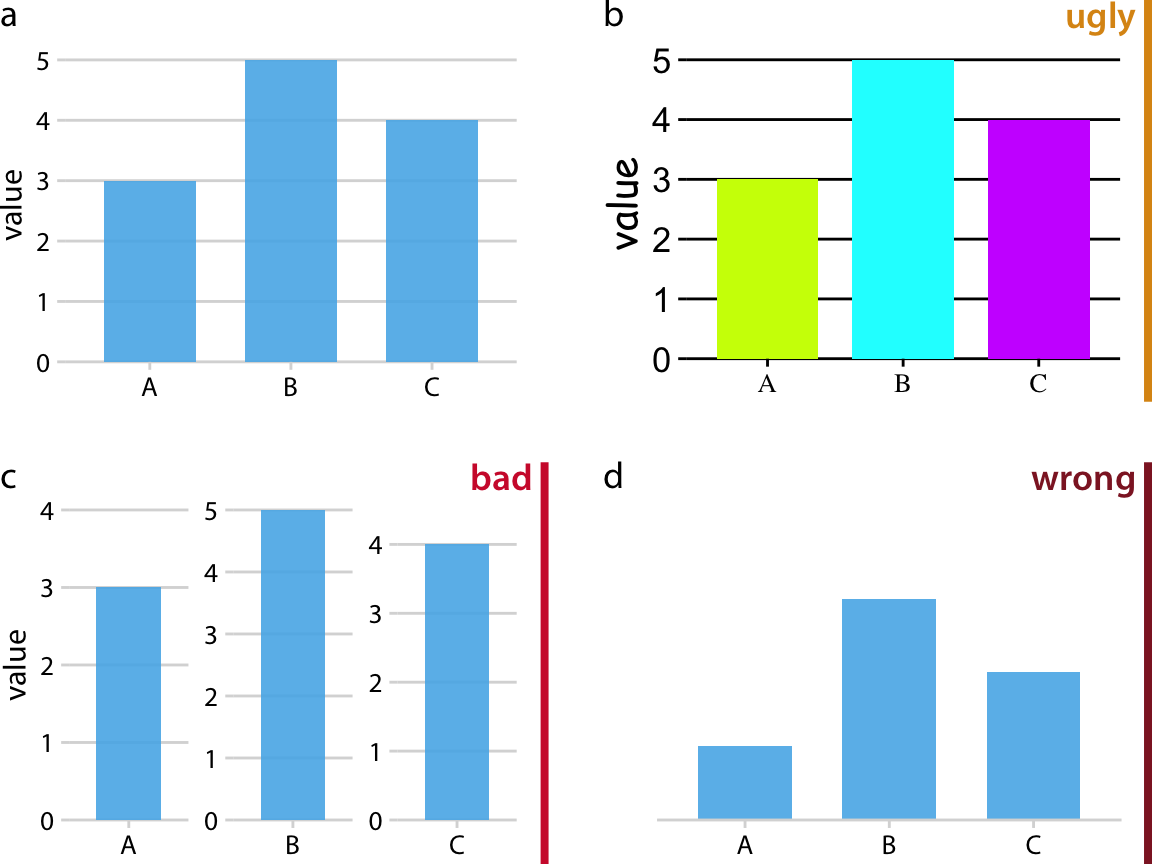
\includegraphics[height=2.5in,width=3.6in]{figuras/fig08}  
\caption{En (a) se muestra  un diagrama de barras para tres valores: A = 3, B = 5 y C = 4;  es una representaci�n sencilla y entendible. (b) es una versi�n fea de la parte (a), aunque el gr�fico es t�cnicamente correcto, es est�ticamente desagradable, con colores innecesarios, una cuadr�cula de fondo absurda y un texto con tipos de letra y tama�os diferentes. (c) es una mala versi�n de la parte (a), en el eje $y$ cada barra tiene  su propia escala y adem�s est�n desalineadas, por lo tanto es una gr�fica enga�osa. (d) es una versi�n incorrecta de la parte (a), como el eje $y$ no pose escalas no es posible determinar sus valores num�ricos.}
\label{estilosfig}
\end{center}
\end{figure}


Cuando se grafican valores experimentales o magnitudes calculadas se debe considerar:

\subsection{Ejes de coordenadas}

En muchas casos, cuando se quiere visualizar datos se necesita definir escalas que permitan posicionar los datos en un gr�fico. En gr�ficos 2D se necesitan dos n�meros para especificar un punto de manera un�voca, es decir, dos escalas de posici�n. Estas dos escalas suelen ser los ejes $x$ (eje horizontal o eje de las abscisas) y el eje $y$ (eje vertical o eje de las ordenadas), es lo generalmente  se denomina el sistema de coordenadas.

\begin{enumerate}
\item En los ejes deben aparecer claramente las magnitudes, s�mbolo o letra, que en ellos se representan y sus unidades de medida correspondientes

\item En los ejes s�lo deben colocarse los valores m�s representativos de la escala escogida.

\item En general, es conveniente que el origen aparezca en el gr�fico, pero no siempre es necesario que la intersecci�n de los dos ejes corresponda al punto cero; en este caso las escalas pueden desplazarse cuando los datos experimentales est�n en un intervalo que as� lo requiera.

\item La variable independiente, cuyo valor lo asigna a conveniencia el experimentador, se representa sobre el eje $x$ horizontal y la variable que depende de ese valor asignado se coloca sobre el eje $y$ vertical.
\end{enumerate}


\subsection{Selecci�n de escalas}
La escogencia de las escalas a utilizar es un problema si no se tiene cuidado al considerar factores como: el tama�o del conjunto de datos, las divisiones sobre cada eje, la relaci�n entre los errores experimentales y los valore m�nimos elegidos en las escalas. 

Las escala no deben ser muy peque�a, ya que en este  caso se  pueden agrupar exageradamente los puntos en una regi�n de la gr�fica (ver figura \ref{escala1}). Tampoco deben elegirse escalas grandes que exageran la precisi�n.
\begin{figure}[h]
\begin{center}
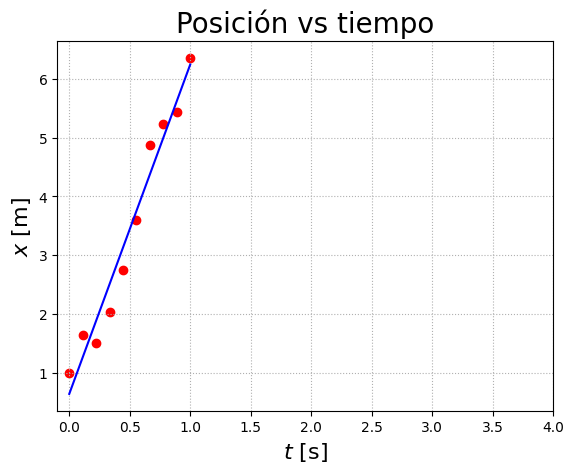
\includegraphics[height=2.5in,width=3.6in]{figuras/fig09}  
\caption{Muy mala selecci�n de las escalas.}
\label{escala1}
\end{center}
\end{figure}

Una gr�fica puede requerir  tener dos ejes que representan dos unidades diferentes, por ejemplo Temperatura en $^\circ$C vs Tiempo en s.  Estirar o comprimir los ejes obedecer� a las razones que necesitemos resaltar, una gr�fica alta y estrecha enfatiza el cambio a lo largo del eje $y$ y una corta y ancha hace lo contrario. Lo ideal es elegir una relaci�n de aspecto que garantice que las diferencias importantes de posici�n sean perceptibles.

Por otro lado, si los ejes $x$ y $y$ se miden en las mismas unidades, entonces las separaciones de la cuadr�cula para los dos ejes deben ser iguales, de forma que la misma distancia a lo largo del eje $x$ o $y$ corresponda al mismo n�mero de unidades de datos.

Los sistemas de coordenadas cartesianos son sistemas de coordenadas lineales y aunque 
suelen proporcionar una representaci�n precisa de los datos, hay situaciones en las que se prefiere utilizar escalas no lineales. En una escala no lineal, a un espaciado uniforme en las unidades de datos le corresponde un espaciado desigual en la visualizaci�n o, contrariamente, a un espaciado uniforme en la visualizaci�n le corresponde un espaciado desigual en las unidades de datos.

La escala no lineal m�s utilizada es la escala logar�tmica o escala logar�tmica abreviada, estas escalas  son lineales en la multiplicaci�n, de forma que un paso unitario en la escala corresponde a una multiplicaci�n con un valor fijo. Para crear una escala logar�tmica, debemos realizar una transformaci�n logar�tmica de los valores de los datos y exponenciar los n�meros que se muestran a lo largo de las l�neas de la cuadr�cula del eje.


\subsection{Ubicaci�n de los puntos}

Los valores experimentales no deben ser graficadas s�lo como un solo punto, se debe representar adem�s el error absoluto con el cual se obtuvo dicho valor. Para ello se usan: cuadrados, rect�ngulos, barras, cruces, etc. (ver figura \ref{barerror}). Si la escala escogida no permite representar el error absoluto, los valores experimentales se deben representar con una equis o una cruz. Las barras de error suelen representarse a lo largo de las direcciones $x$ y  $y$ en un gr�fico de dispersi�n.

En las figuras 2D sencillas, las barras de error tienen una ventaja importante sobre las representaciones m�s complejas de la incertidumbre ya que se pueden combinar con muchos otros tipos de gr�ficos. Por lo tanto, las barras de error resultan ser la representaciones m�s sencillas para mostrar cantidades con incertidumbre sobre todo en las gr�ficas de barras. 

Cada conjunto debe ser representado por un s�mbolo diferente, por ejemplo: $\times, \Delta, \odot,+$ e identificar luego cada curva. La recta o curva que siguen los puntos se debe trazar de un modo que la funci�n sea lo m�s representativa posible del comportamiento de las magnitudes que caracterizan el fen�meno  en estudio.
\begin{figure}[h]
\begin{center}
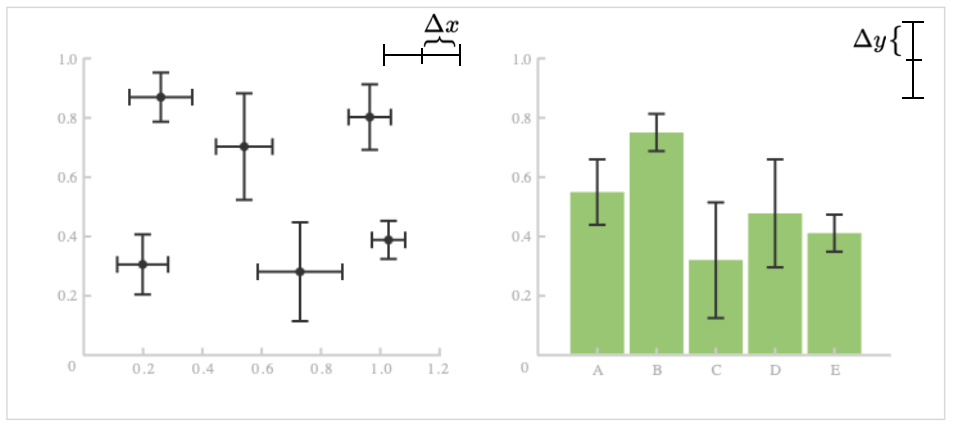
\includegraphics[height=2.2in,width=4.6in]{figuras/fig11}  
\caption{Representaci�n de puntos experimentales con barras de error.}
\label{barerror}
\end{center}
\end{figure}


\section{Trazado de una recta}

En algunos experimentos las magnitudes f�sicas pueden variar linealmente, como es el caso de la deformaci�n y la fuerza en la ley de Hooke $(F = -kx)$. Al realizar el experimento y graficar resulta  un conjunto de puntos que corresponde a un comportamiento lineal. 

El experimentador tiene que buscar ahora la mejor estrategia  para trazar la mejor recta que pasa por entre los puntos experimentales.

Los m�todos estad�sticos demuestran que, siempre que la dispersi�n de los puntos experimentales  se deba a los errores casuales de medici�n, la mejor recta pasar� por el centroide de los puntos experimentales, que es el punto con las coordenadas
$(\bar{x}, \bar{y})$, en donde $\bar{x}$ y $\bar{y}$  son los  valores medios de las coordenadas $x$ y $y$ respectivamente.
\begin{equation}
\begin{aligned}
\bar{x} & =\frac{1}{n}{\sum_{i=1}^n x_i} \\
\bar{y} & =\frac{1}{n}{\sum_{i=1}^n y_i}
\end{aligned}
\end{equation}


Para ajustar la recta al conjunto de puntos experimentales, se emplear�n los siguientes m�todos:

\subsection{M�todo gr�fico}
Este m�todo es un m�todo artesanal, y consiste en buscar sobre la gr�fica la mejor recta que pase  por el centroide y la mayor�a de los puntos experimentales. Aquellos puntos que queden por fuera de esta recta deben estar distribuidos en lo posible con igual peso a ambos lados de la curva.

Como sabemos, la ecuaci�n de una recta es:
$$
y=m x+b
$$
donde:
\begin{itemize}
\item $m$ es la pendiente de la recta, calculada a partir de las coordenadas de dos puntos sobre la recta, necesariamente no tienen que corresponder a valores experimentales.
$$
m=\frac{\left(y_2-y_1\right)}{\left(x_2-x_1\right)} \frac{\text { unidad de } y}{\text { unidad de } x}
$$
\item  $b$ es el corte de la recta con el eje de las ordenadas en $x=0$.
\end{itemize}

El error absoluto para $m$ y $b$ viene dado por la lectura de la posici�n de los puntos sobre el gr�fico, es decir en funci�n de la apreciaci�n de la escala en el eje respectivo.


\subsection{M�todo de los m�nimos cuadrados}

El m�todo de los m�nimos cuadrados es uno de los m�todos estad�sticos m�s usados para determinar la recta que mejor represente la tendencia de un conjunto de puntos experimentales.

Si la dispersi�n de los puntos experimentales es debida solo a los errores casuales en las mediciones, la mejor recta ser� aquella para la cual la suma de los cuadrados de las distancias $\left(y_i-y_0 \right)$ sea un m�nimo, ver figura 4.4. Es por esto que, a este m�todo se le llama m�todo de los m�nimos cuadrados.

Consideremos una relaci�n lineal entre dos magnitudes f�sicas $y$ y $x$ de la forma:
$$
y=m x+b
$$

Donde $y$ es la variable dependiente y $x$ es la variable independiente, en nuestro caso la magnitud controlada por el experimentador. Como ya se ha dicho anteriormente, los valores de esas magnitudes tendr�n sus correspondientes errores, determinados por los m�todos ya se�alados. 

La desviaci�n de un valor cualquiera $y_i$ determinado experimentalmente con respecto a su valor $y_0$ en la recta, ser�:
\begin{equation}
\Delta y_i=y_i-y_0=y_i-\left(b+m x_i\right)
\label{deltay}
\end{equation}

Ahora se puede enunciar el principio b�sico de este m�todo, el cual dice que:

La mejor recta que puede ser trazada entre esos puntos, es aquella para la cual la suma de los cuadrados de las desviaciones $\Delta y_i$ de los datos experimentales, con respecto a esa recta, es m�nima.
$$
\sum_{i=1}^n\left(\Delta y_i\right)^2=\sum_{i=1}^n \left[y_i-b-m x_i \right]^2
$$
donde $n$ es el n�mero de pares de valores de $y$ y $x$.

Ya que la condici�n exigida es la de minimizar la suma anterior, entonces los par�metros $m$ y $b$ deben ajustarse para cumplir con esta condici�n. Ello se logra calculando las derivadas parciales de la suma con respecto a $m$ y con respecto a $b$, e igual�ndolas a cero.
$$
\begin{aligned}
& \frac{\partial\left[\sum\left(\Delta y_i\right)^2\right]}{\partial b}=
\sum_{i=1}^n\frac{\partial\left(y_i-b-m x_i \right)^2}{\partial b} = 
\sum_{i=1}^n -2(y_i-b-m x_i)=0  \\
& \frac{\partial\left[\sum\left(\Delta y_i\right)^2\right]}{\partial m}=
\sum_{i=1}^n\frac{\partial\left(y_i-b-m x_i \right)^2}{\partial m} =
\sum_{i=1}^n -2x_i(y_i-b-m x_i)=0
&
\end{aligned}
$$

Por lo tanto, se debe resolver el sistema 
$$
\begin{aligned}
&  \sum_{i=1}^n y_i - \sum_{i=1}^nb - \sum_{i=1}^n m x_i = 0  &\,\, \Rightarrow \,\,&
 nb + m \sum_{i=1}^n  x_i = \sum_{i=1}^n y_i  \\
&  \sum_{i=1}^n y_ix_i - \sum_{i=1}^n bx_i -\sum_{i=1}^n  m x_i^2 =0 & \,\, \Rightarrow \,\,&
b \sum_{i=1}^n x_i  + m \sum_{i=1}^n   x_i^2 = \sum_{i=1}^n y_ix_i
\end{aligned}
$$
para $m$ y $b$. 

Utilizando la regla de Cramer
$$
\begin{aligned}
\Delta= 
{\left|\begin{array}{cc}
n & \sum x_i \\
\sum x_i & \sum x_i^2
\end{array}\right|} = n \sum x_i^2-\left(\sum x_i\right)^2 \,,
\end{aligned}
$$

$$
\begin{aligned}
& b=\frac{\left|\begin{array}{cc}
\sum y_i & \sum x_i \\
\sum x_i y_i & \sum x_i^2 
\end{array}\right|}{\Delta}=\frac{\sum x_i^2 \sum y_i-\sum x_i \sum x_i y_i}{n \sum x_i^2-\left(\sum x_i\right)^2} \\ \\
& m=\frac{\left|\begin{array}{cc}
n & \sum y_i \\
\sum x_i & \sum x_i y_i
\end{array}\right|}{\Delta}=\frac{n\sum x_i y_i-\sum x_i \sum y_i}{n \sum x_i^2-\left(\sum x_i\right)^2}
\end{aligned}
$$

Por lo tanto:
\begin{eqnarray}
b &=&\dfrac{\sum\limits_{i=1}^n x_i^2 \sum\limits_{i=1}^n y_i-\sum\limits_{i=1}^n x_i \sum\limits_{i=1}^n x_i y_i}{n\sum\limits_{i=1}^n x_i^2-\left(\sum\limits_{i=1}^n x_i\right)^2} 
\label{emeyb1}\\
m &=&\dfrac{ n\sum\limits_{i=1}^n x_i y_i-\sum\limits_{i=1}^n x_i \sum\limits_{i=1}^n y_i}{n \sum\limits_{i=1}^n x_i^2-\left(\sum\limits_{i=1}^n x_i\right)^2}
\label{emeyb2}
\end{eqnarray}

De esta manera obtenemos la recta $f(x)=mx+b$ que mejor de aproxima a los puntos. 

N�tese que los t�rminos $\sum x_i^2$ y $\left(\sum x_i\right)^2$ no son lo mismo. Id�ntica observaci�n se debe hacer para los t�rminos $\sum\left(x_i y_i\right)$ y $\sum x_i \sum y_i$.

Es recomendable construir una tabla como \ref{tablamincua}, para as� ordenar la informaci�n y facilitar los c�lculos. Las cuatro sumas en la �ltima l�nea, son los valores necesarios para calcular $m$ y $b$. Los valores de $m$ y $b$ que se obtengan por el m�todo de los m�nimos cuadrados, deber�an ser muy pr�ximos a los obtenidos directamente utilizando el m�todo gr�fico.
\begin{table}[h]
\begin{center}
\begin{tabular}{|c|c|c|c|}
\hline $y_i [\,\,]$ & $x_i [\,\,]$ & $x_i^2 [\,\,]$& $x_i y_i [\,\,]$ \\
\hline \hline $y_1$ & $x_1$ & $x_1^2$ & $x_1 y_1$ \\
\hline $\vdots$ & $\vdots$ & $\vdots$ & $\vdots$ \\
\hline $\vdots$ & $\vdots$ & $\vdots$ & $\vdots$ \\
\hline $y_n$ & $x_n$ & $x_n^2$ & $x_n y_n$ \\ \hline
\hline $\sum y_i$ &$\sum x_i $& $\sum x_i^2$ & $\sum x_i y_i$ \\
\hline
\end{tabular}
\end{center}
\caption{Tabla para facilitar el uso del  m�todo de m�nimos cuadrados}
\label{tablamincua}
\end{table}


Actualmente es casi de rutina utilizar alguna herramienta computacional  que permite hacer los c�lculos necesarios y los gr�ficos para el ajuste de la recta. Aunque el uso de este m�todo no nos obliga a hacer el gr�fico de la recta, por razones pedag�gicas, es conveniente hacerlo para as� observar m�s claramente las desviaciones de los puntos experimentales con respecto a la recta calculada. 

Una vez obtenido los valores de $m$ y ${b}$, es necesario calcular sus errores correspondientes $\Delta m$ y $\Delta b$. Esto lo podemos hacer calculando las desviaciones est�ndar  de la pendiente y la ordenada al origen, calculadas a partir de la distribuci�n de diferencias $\Delta y_i$, ecuaci�n (\ref{deltay}),  respecto de la mejor l�nea de ajuste. Sea  $S_y$  la  desviaci�n est�ndar de $y$ respecto a la l�nea recta obtenida por m�nimos cuadrados:
\begin{equation}
S_y=\left[\frac{\sum\limits_{i=1}^n \left(y_i-b-m x_i\right)}{n-2}\right]^{\frac{1}{2}} \,.
\end{equation}

Para calcular estos valores de $\Delta m$ y $\Delta b$ se utilizan las siguientes expresiones:
\begin{eqnarray}
\Delta m & =\left[\frac{n}{n \sum\limits_{i=1}^n\left(x_i\right)^2-\left(\sum\limits_{i=1}^n x_i\right)^2}\right]^{\frac{1}{2}} S_y 
\label{Delm}\\
\Delta b & =\left[\frac{\sum\limits_{i=1}^n\left(x_i\right)^2}{n \sum\limits_{i=1}^n\left(x_i\right)^2-\left(\sum\limits_{i=1}^n x_i\right)^2}\right]^{\frac{1}{2}} S_y
\label{Delb}
\end{eqnarray}

La cantidad $S_y$ representa la llamada desviaci�n est�ndar de $y$ respecto a la l�nea recta obtenida.

Finalmente para calcular $S_y$ se puede utilizar como ayuda la tabla \ref{tablamincua2}
\begin{table}[h]
\begin{center}
\begin{tabular}{|c|c|c|c|}
\hline$x_i [\,\,]$ & $y_i [\,\,]$ & $y_i-m x_i-b$ & $(y_i-m x_i-b)^2$ \\
\hline \hline$x_1$ & $y_1$ & $y_1-m x_1-b$ & $\left(y_1-m x_1-b\right)^2$ \\
\hline$x_2$ & $y_2$ & $y_2-m x_2-b$ & $\left(y_2-m x_2-b\right)^2$ \\
\hline$\vdots$ & $\vdots$ & $\vdots$ & $\vdots$ \\
\hline$\vdots$ & $\vdots$ & $\vdots$ & $\vdots$ \\
\hline$x_n$ & $y_n$ & $y_n-m x_n-b$ & $\left(y_n-m x_n-b\right)^2$ \\ \hline
\hline & & & $\sum\limits_{i=1}^n \qquad \qquad \quad$ \\
\hline
\end{tabular}
\end{center}
\caption{Tabla para facilitar los c�lculos de $S_y$.}
\label{tablamincua2}
\end{table}

\paragraph{Ejemplo 7.}

En un experimento sobre cinem�tica un grupo de estudiantes mide los tiempos con los que se desplaza  un m�vil en un riel de aire. Lis tiempos son medidos en segundos usando un cron�metro de sensibilidad $S=0,01$ s. Un instrumento de mejor precisi�n mide las velocidades con las que se desplaza el m�vil, este instrumento tiene una sensibilidad de $0,001$ m/s.  Los datos se muestran en la tabla \ref{datos1}.
\begin{table}[h]
\begin{center}
\begin{tabular}{|c|c|}
\hline $t_i \pm 0,01 (\mathrm{s})$ & $v_i \pm 0,01 (\mathrm{m/s})$  \\\hline \hline 
\hline $0,00$ & 1.00 \\
\hline $0,10$ & 1.64 \\
\hline $0,20$ & 1.51 \\
\hline $0,30$ & 2.03 \\
\hline $0,40$ & 2.75 \\
\hline $0,50$ & 3.59 \\
\hline $0,60$ & 4.87 \\
\hline $0,70$ & 5.23 \\
\hline $0,80$ & 5.44 \\
\hline $1,00$ & 6.37 \\
\hline
\end{tabular}
\end{center}
\caption{Mediciones de la velocidad de un cuerpo en funci�n del tiempo}
\label{datos1}
\end{table}

Al graficar los datos anteriores se obtiene la figura
\begin{figure}[h]
\begin{center}
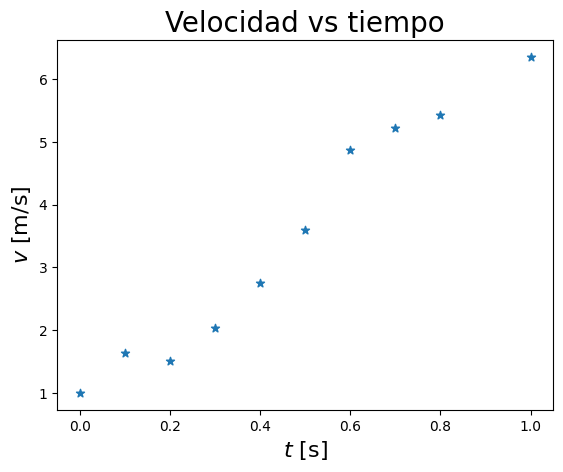
\includegraphics[height=2.5in,width=2.5in]{figuras/fig12}  
\caption{Gr�fico de los datos $v$ vs $t$ de la tabla \ref{datos1}.}
\label{figdatos1}
\end{center}
\end{figure}

Es recomendable calcular las siguientes sumas:
$$
\begin{array}{c|c|c|c|c}
n&\sum_{i=1}^n t_i & \sum_{i=1}^n v_i   & \sum_{i=1}^n t_i^2  & \sum_{i=1}^n t_i v_i \\ \hline\hline 
10 & 4.60 & 34.43 & 3.04 & 21.3
\end{array}
$$
$$
\Delta=n\sum\limits_{i=1}^n t_i^2-\left(\sum\limits_{i=1}^n t_i\right)^2= 
10(3.04) - \left(4.60 \right)^2= 9.24 \,\, \mathrm{s}^2
$$
$$
b=\dfrac{\sum\limits_{i=1}^n t_i^2 \sum\limits_{i=1}^n v_i-\sum\limits_{i=1}^n t_i \sum\limits_{i=1}^n t_i v_i}{\Delta} =
\frac{(3.04)  (34.43) -(4.60) (21.3)}{9.24} = 0.724 \,\, \mathrm{m/s}
$$
$$
m =\dfrac{n \sum\limits_{i=1}^n t_i v_i-\sum\limits_{i=1}^n t_i \sum\limits_{i=1}^n v_i}{\Delta} =\frac{10(21.3)  -(4.60) ( 34.43)}{9.24}= 5.91\,\, \mathrm{m/s^2}
$$

Procedemos a calcular los errores 
$$
\begin{array}{c|c}
n& \sum\limits_{i=1}^n \left(v_i-b-m t_i\right)  \\ \hline\hline 
10 & 6.63 
\end{array}
$$
La desviaci�n est�ndar de $y$:
$$
S_y=\left[\frac{\sum\limits_{i=1}^n \left(v_i-b-m t_i\right)^2}{n-2}\right]^{\frac{1}{2}}=
\left(\frac{6.63}{8}\right)^{\frac{1}{2}}=0.91 \,.
$$
y los errores 
$$
\begin{aligned}
\Delta m & =\left[\frac{n}{\Delta}\right]^{\frac{1}{2}} S_y = \left[\frac{10}{9.24}\right]^{\frac{1}{2}} (0.91)=0.95 \\
\Delta b & =\left[\frac{\sum\limits_{i=1}^n\left(t_i\right)^2}{\Delta}\right]^{\frac{1}{2}} S_y= 
\left[\frac{3.04}{9.24}\right]^{\frac{1}{2}} (0.91)= 0.52
\end{aligned}
$$

Por lo tanto nuestro resultado ser�:
$$
v=mt + b= 5.91 t + 0.724 \,\, \mathrm{m/s}
$$
donde $m=5.91 \pm 0.95$ y $b=0.72 \pm 0.52$.

En Python podemos hacer todos los casos anteriores, incluida la figura \ref{figdatos1}, pero primero debemos ingresar los datos
\begin{lstlisting}[language=Python]    
yn=  array([1.000, 1.64, 1.51, 2.03, 2.75, 3.59, 4.87, 5.23, 5.44, 6.37])
xn = array([0.00, 0.10, 0.20, 0.30, 0.40, 0.50, 0.60, 0.70, 0.80, 1.00])
\end{lstlisting}

La gr�fica de la figura \ref{figdatos1} se obtiene a partir de las siguientes lineas de c�digo:
\begin{lstlisting}[language=Python] 
plt.scatter(xn, yn, marker='*')
plt.title(r'Velocidad vs tiempo', fontsize=20)
plt.xlabel(r'$t$ [s]', fontsize=16)
plt.ylabel(r'$v$ [m/s]', fontsize=16)
\end{lstlisting}

Para usar las ecuaciones (\ref{emeyb1})-(\ref{emeyb2}) hagamos primero los siguientes c�lculos intermedios
\begin{lstlisting}[language=Python] 
#Se obtiene el valor de n (numero de datos)
n=len(xn)
#Las sumatorias necesarias 
Sum_x=sum(xn)
Sum_y=sum(yn)
Sum_xx=sum(xn**2)
Sum_xy=sum(xn*yn)
print(n,',', Sum_x, ',',Sum_y,',', Sum_xx,',', Sum_xy)
\end{lstlisting}
\begin{tcolorbox}[width=\textwidth,colback={ghostwhite}]   
{\small 
10 , 4.6 , 34.43 , 3.04 , 21.275
}
\end{tcolorbox} 

Y finalmente calculamos $b$ y $m$
\begin{lstlisting}[language=Python] 
# Se escriben las ecuaciones para b y m 
b=(Sum_xx*Sum_y-Sum_xy*Sum_x)/(n*Sum_xx-Sum_x**2)
m=(n*Sum_xy-Sum_x*Sum_y)/(n*Sum_xx-Sum_x**2)
print('m=',m, ',', 'b=',b)
\end{lstlisting}
\begin{tcolorbox}[width=\textwidth,colback={ghostwhite}]   
{\small 
m= 5.884415584415585 , b= 0.7361688311688325
}
\end{tcolorbox} 

Notemos lo diferente del valor de $m$ con respecto al obtenido anteriormente, esta diferencia obviamente se debe a que anteriormente fuimos haciendo redondeos en la operaciones. 

Veamos la recta y los datos
\begin{lstlisting}[language=Python] 
# La gr�fica con los datos y la recta que mejor se ajusta 
x=xn
y=m*x+b
#
plt.scatter(xn, yn, color='b',marker='+')
plt.grid(linestyle='dotted')
plt.plot(x, y, color='r')
plt.title(r'Velocidad vs tiempo', fontsize=20)
plt.xlabel(r'$t$ [s]', fontsize=16)
plt.ylabel(r'$v$ [m/s]', fontsize=16)
plt.xlim(-0.1, 1.1)
plt.text(0.6, 1.0, '$y=(5.88) x + 0.736$', fontsize=12)
plt.show()
\end{lstlisting}
\begin{figure}[h]
\begin{center}
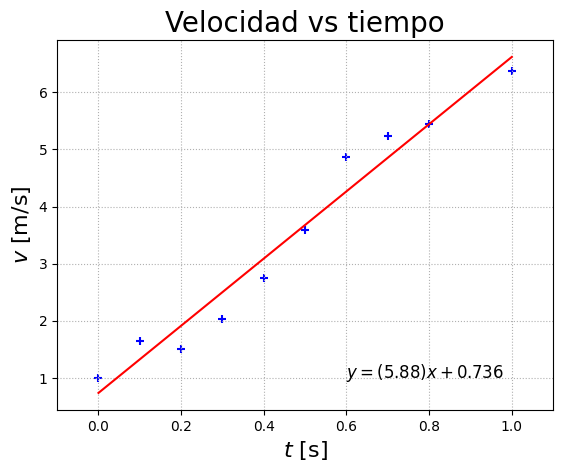
\includegraphics[height=2.6in,width=3.0in]{figuras/fig13}  
\label{figdatos2}
\end{center}
\end{figure}

El siguiente paso es calcular $\Delta b$ y $\Delta m$

\begin{lstlisting}[language=Python] 
# Escribimos las sumatorias para calcular Sy
Sum_d= Sum_y-b-m*Sum_x
Sy=sqrt(Sum_d/(n-2))
print(n,',', Sum_d,',', Sy)
\end{lstlisting}
\begin{tcolorbox}[width=\textwidth,colback={ghostwhite}]   
{\small 
10 , 6.625519480519479 , 0.9100494135292516
}
\end{tcolorbox}

Los respectivos errores se obtienen de las ecuaciones (\ref{Delm}) y (\ref{Delb}) 

\begin{lstlisting}[language=Python] 
Dm= (n/((n*Sum_xx-Sum_x**2)))**(1/2)*Sy
Db= (Sum_xx/((n*Sum_xx-Sum_x**2)))**(1/2)*Sy
print('Dm=', Dm, ',', 'Db=',Db)
\end{lstlisting}
\begin{tcolorbox}[width=\textwidth,colback={ghostwhite}]   
{\small 
Dm= 0.9467362111662778 , Db= 0.5219943236034063
}
\end{tcolorbox}

Por lo tanto:
$$
v= 5.88 t + 0.736 \,\, \mathrm{m/s}
$$
donde: $m=5.88 \pm 0.95$ y $b=0.74 \pm 0.52$.



\section{An�lisis Gr�fico de Funciones}
En el an�lisis de un experimento generalmente se dispone de un conjunto de datos que de acuerdo a la teor�a del fen�meno en estudio debe corresponder a una cierta ley f�sica. ley  que se expresa mediante una ecuaci�n matem�tica.  Este an�lisis se puede lograr graficando los valores experimentales que seguramente seguir�n una cierta curva que corresponde a la tendencia de los puntos.  La idea es comparar la forma de la curva obtenida por la mediciones con la predicha por la teor�a. Si la comparaci�n muestran la misma tendencia se concluye que esto es una comprobaci�n experimental de la teor�a considerada.

Como es m�s f�cil obtener la informaci�n de un gr�fico lineal, entonces se procede a elegir convenientemente las variables de modo de obtener una funci�n lineal. A continuaci�n se mostrar� como algunas de las funciones m�s conocidas pueden ser llevadas a un gr�fico lineal.

\subsection{Funci�n exponencial}
Dada la funci�n 
\begin{equation}
y(x)=k a^{b x}
\label{funexp}
\end{equation}
donde $k, a$ y $b$ son constantes. Si  $b>0$  la exponencial es creciente, mientras que si si $b < 0$, la exponencial es decreciente. Notemos  que en $x=0$, $y=k$, por lo que $k$ resulta ser la ordenada al origen, es decir, la curva intercepta al eje de las ordenadas en el punto $(0, k)$.

Tomando logaritmos se tiene:
\begin{equation}
\log (y)=b \log(a) x +\log (k)
\label{funexplin}
\end{equation}
Recordemos que si por ejemplo $a=10$ debemos tomar  logaritmo en base diez. 

Si hacemos una gr�fica directamente $\log y$ en funci�n de $x$  se obtendr� una recta, pero para ello habr�a que calcular los logaritmos de $y$. Este c�lculo puede ser evitado usando un papel especial llamado papel semi-logar�tmico, en el cual uno de los ejes tiene las divisiones proporcionales a los logaritmos decimales y el otro es lineal. 

En la escala logar�tmica existen ciclos, donde un ciclo corresponde al conjunto de n�meros entre dos potencias de diez (1 a $10; 10$ a $100; 100$ a 1000 � 0,1 a 1; etc.).

El gr�fico de la funci�n $y=k a^{bx}$ es una recta porque la ecuaci�n (\ref{funexplin}) puede ser escrita como
$$
u=m x+v \,,
$$
donde: $u =\log(y)$,  $m =b \log(a)$ y  $v=\log (k)$.

Para calcular la pendiente de la recta hay que considerar que se est� trabajando con logaritmos:
$$
\text {pendiente}=m=\frac{u_2-u_1}{x_2-x_1}  =\frac{\log y_2-\log y_1}{x_2-x_1}=b \log a
$$

Es de hacer notar que al graficar en papel semi-logar�tmico y llevar los valores en la escala logar�tmica, se llevan directamente los n�meros a la escala y no se calculan los logaritmos, pero al calcular la pendiente si es necesario hacerlo. Adem�s si se est� utilizando papel semi-logar�tmico, $k$ es el corte de la recta en $x=0$.

En las siguientes lineas de c�digo podemos interpretar lo expuesto anteriormente tomando la funci�n exponencial siguiente:
$$
y = 5\cdot 10^{\frac{x}{3}}
$$
cuya gr�fica la podemoa hacer de la manera siguiente
\begin{lstlisting}[language=Python] 
x = arange(10)
y = 5*10**(1/3*x)
plt.plot(x, y, 'o')
plt.show()
\end{lstlisting}
\begin{figure}[h]
\begin{center}
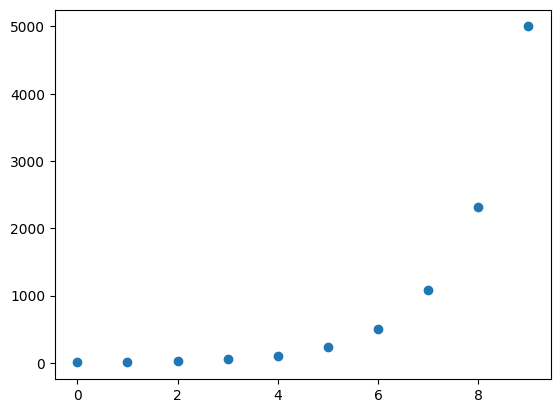
\includegraphics[height=2.4in,width=2.9in]{figuras/fig14}  
\label{figexp1}
\end{center}
\end{figure}

Ahora la funci�n lineal pero en escala logar�tmica
\begin{lstlisting}[language=Python] 
plt.plot(x, y, '-o')
plt.yscale("log")
plt.show()
\end{lstlisting}
\begin{figure}[h]
\begin{center}
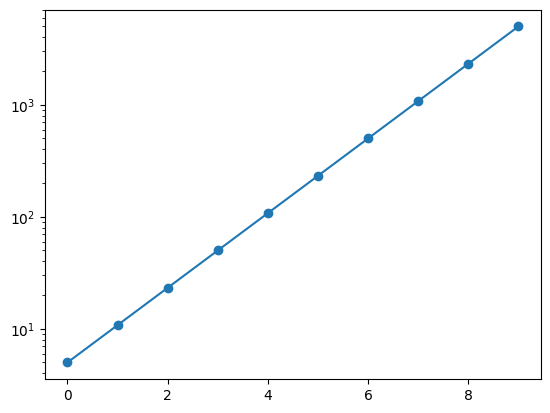
\includegraphics[height=2.4in,width=2.9in]{figuras/fig15}  
\label{figexp1lin}
\end{center}
\end{figure}

\newpage
\subsection{Funci�n potencial}
Dada la funci�n:
\begin{equation}
y= c x^m
\label{funpot}
\end{equation}
donde $m$ y $c$ son constantes. 

Tomando logaritmos decimales  se tiene:
\begin{equation}
\log (y)=m \log (x)+\log (c)
\label{funpotlin}
\end{equation}

Si se hace una gr�fica directamente $\log y$ en funci�n de $\log x$ se obtendr� una recta, pero habr�a que calcular los logaritmos decimales de $y$ y de $x$. Esto se puede  evitar  usando un papel especial llamado papel logar�tmico (com�nmente llamado $\log-\log$ ), el cual tiene ambas escalas proporcionales a los logaritmos decimales.

El gr�fico de la funci�n $y=c x^m$ es una recta porque la ecuaci�n (\ref{funpotlin}) se puede escribir como:
$$
v=m u+k \,,
$$
donde: $v =\log(y) $, $u=\log(x) $ y $k=\log(c)$

La pendiente $m$ de la recta est� dada por:
$$
m =\frac{v_2-v_1}{u_2-u_1}  =\frac{\log y_2-\log y_1}{\log x_2-\log x_1}=\frac{\log \left(\frac{y_2}{y_1}\right)}{\log \left(\frac{x_2}{x_1}\right)}
$$
y $c$ representa el corte de la recta en $x=1(\log 1=0)$.

Consideremos la  funci�n potencial siguiente:
$$
y = 8\ x^{3}
$$

Procedemos a realizar su gr�fica:
\begin{lstlisting}[language=Python] 
x = arange(20)
y = 8*x**(3)
plt.plot(x, y, '*')
plt.show()
\end{lstlisting}
\begin{figure}[h]
\begin{center}
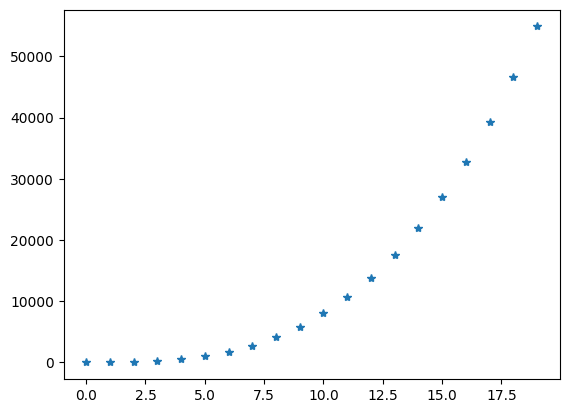
\includegraphics[height=2.4in,width=2.9in]{figuras/fig16}  
\label{figexp1}
\end{center}
\end{figure}
\newpage

Ahora la funci�n lineal pero en escala log-log
\begin{lstlisting}[language=Python] 
plt.plot(x, y, '-*')
plt.xscale("log")
plt.yscale("log")
plt.show()
\end{lstlisting}
\begin{figure}[h]
\begin{center}
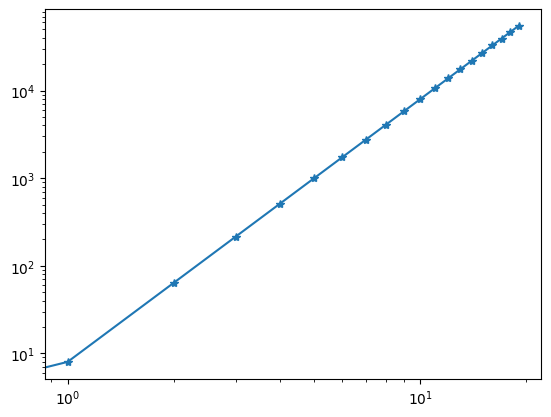
\includegraphics[height=2.4in,width=2.9in]{figuras/fig17}  
\label{figexp1lin}
\end{center}
\end{figure}




\chapter{Regresi�n lineal}

\section{Introducci�n}

Este cap�tulo lo dedicamos al  an�lisis de regresi�n, que es una t�cnica estad�stica utilizada para investigar y modelar la relaci�n entre variables. Los m�todos de an�lisis de regresi�n tienen una gran cantidad de aplicaciones en ingenier�a, ciencias f�sicas y qu�micas, econom�a, ciencias de la vida y las ciencias sociales. Otro campo de aplicaci�n es la ciencia y an�lisis de datos, esto hace que el espectro de problemas donde se aplica el an�lisis de regresi�n sea muy amplio.

El an�lisis de regresi�n fue desarrollado por primera vez por Sir Francis Galton\footnote{Francis Galton 1822-1911. \url{https://en.wikipedia.org/wiki/Francis_Galton}} a finales del siglo XIX. Galton redescubri� de forma independiente el concepto de correlaci�n y demostr� su aplicaci�n en el estudio de la herencia, la antropolog�a y la psicolog�a. Galton desarroll� una descripci�n matem�tica de la tendencia regresiva, precursora de los modelos de regresi�n actuales y el t�rmino regresi�n sigue utiliz�ndose para describir las relaciones estad�sticas entre variables.

\section{Regresi�n y la construcci�n de modelos}
El an�lisis de regresi�n es una t�cnica estad�stica que permite investigar y construir modelos que establecen relaciones entre variables.

Las relaciones estad�sticas son diferentes de las  relaciones funcionales porque las relaciones estad�sticas no son perfectas, es decir, las observaciones de una relaci�n estad�stica no caen directamente sobre una curva de relaci�n. 

Supongamos que observamos una respuesta cuantitativa $y$ para  $k$ ``predictores'' diferentes: $x_1, x_2, \ldots, x_k$. Podemos suponer tambi�n que existe alguna relaci�n entre $y$ y $x=\left(x_1, x_2, \ldots, x_k\right)$, que puede escribirse de la forma muy general
\begin{equation}
y=f(x)+\varepsilon \,.
\label{funcion}
\end{equation}
donde $f$ es alguna funci�n fija pero desconocida de $x_1, \ldots, x_k$, y $\varepsilon$ es un t�rmino de error aleatorio, que es independiente de $x$ y tiene media cero. En esta formulaci�n, $f$ representa la informaci�n sistem�tica que $x$ proporciona sobre $y$.

Existen dos razones principales para querer estimar $f$: la predicci�n y la inferencia. 

\paragraph{Predicci�n:} Aqu� hablamos en el proceso de usar un modelo estad�stico o de aprendizaje autom�tico para predecir valores futuros o no observados basados en datos existentes. El objetivo principal de la predicci�n es obtener valores precisos de la variable de inter�s y la precisi�n de las predicciones es el criterio m�s importante. En este caso, es com�n encontrarse en situaciones donde se dispone f�cilmente de un conjunto de entradas $x$, pero no es posible obtener de manera sencilla la salida $y$. En este escenario, dado que el t�rmino de error es igual a cero, podemos predecir $y$ utilizando
$$
\hat{y} = \hat{f}(x)\,,
$$
donde $\hat{f}$ representa nuestra estimaci�n de $f$, y $\hat{y}$ es la predicci�n resultante para $y$. En este contexto, podemos considerar a $\hat{f}$ como una caja negra, en el sentido de que no nos preocupa la forma exacta de $\hat{f}$, siempre y cuando genere predicciones precisas para $y$.  En general, $\hat{f}$ no ser� una estimaci�n perfecta de $f$, y esta imprecisi�n introducir� alg�n error. Este error puede ser reducible si logramos mejorar la precisi�n de $\hat{f}$ utilizando una t�cnica de aprendizaje estad�stico m�s adecuada para estimar $f$. Si pudi�semos construir una predicci�n perfecta de $f$, de manera que $\hat{y} = f(x)$, esta predicci�n a�n tendr�a error porque en realidad $y$ es una funci�n de $\varepsilon$, que es de car�cter aleatorio. Esto se conoce como error irreducible, ya que por muy bien que estimemos $f$, no podemos reducir el error introducido por $\varepsilon$. 

Los m�todos m�s utilizados para la predicci�n son la regresi�n lineal, los �rboles de decisi�n, las redes neuronales, m�todos que podr�amos usas si queremos predecir precios en la bolsa de valores o el valor de un determinado producto bajo determinadas condiciones.


\paragraph{Inferencia:} Aqu� el objetivo no es necesariamente hacer predicciones para $y$ al estimar $f$, sino conocer $f$ de manera exacta. Se refiere al proceso de usar un modelo estad�stico para entender la relaci�n entre las variables y sacar conclusiones sobre la poblaci�n de la cual se extrajo la muestra. El objetivo principal de la inferencia es realizar afirmaciones sobre los par�metros del modelo y sobre la naturaleza de las relaciones entre las variables. En este contexto, podr�amos preguntarnos si existe una relaci�n entre $y$ y cada predictor que tome la forma de una ecuaci�n lineal, o si se trata de una relaci�n m�s compleja. Hist�ricamente, la mayor�a de los m�todos para estimar $f$ han adoptado una forma lineal. En algunas situaciones, este supuesto es razonable o incluso deseable. Sin embargo, a menudo la relaci�n verdadera es m�s complicada, en cuyo caso un modelo lineal puede no proporcionar una representaci�n precisa de la relaci�n entre las variables de entrada y de salida. 

Los m�todos m�s utilizados en la inferencia son las pruebas de hip�tesis, estimaci�n de los intervalos de confianza, el an�lisis de varianza (ANOVA), la regresi�n lineal m�ltiple. Estas t�cnicas pueden usarse para un estudio estad�stico para inferir si existe una relaci�n entre el consumo de caf� y el riesgo de padecer diabetes. 

Es muy probable encontrar situaciones que se encuadren en el �mbito de la predicci�n, en el de la inferencia, o en una combinaci�n de ambos. Por ejemplo, los modelos lineales permiten una inferencia relativamente sencilla e interpretable, pero pueden no producir predicciones tan precisas como otros enfoques. Por el contrario, algunos de los enfoques no lineales pueden proporcionar predicciones bastante precisas para $y$, pero a costa de un modelo menos interpretable, haciendo la inferencia m�s dif�cil.


Uno de los m�todos m�s utilizados para estimar $f$ es el ``m�todo param�trico'', donde, en primer lugar, se hace una suposici�n sobre la forma funcional de $f$. Por ejemplo, una suposici�n muy simple es que $f$ es lineal en $x$:
\begin{equation}
f(x)=\beta_0+\beta_1 x_1+\beta_2 x_2+\cdots+\beta_k x_k \,, 
\label{modlineal}
\end{equation}
En este caso, el problema de estimar $f$ se simplifica enormemente, ya que en lugar de tener que estimar una funci�n $k$-dimensional completamente arbitraria $f(x)$, solo hay que estimar los coeficientes $\beta_0, \beta_1, \ldots, \beta_k$. Y en segundo lugar, una vez seleccionado un modelo, necesitamos un procedimiento que utilice los datos para ajustar o entrenar el modelo. En el caso del modelo lineal (\ref{modlineal}), necesitamos estimar los par�metros \( \beta_0, \beta_1, \ldots, \beta_k \). Es decir, queremos encontrar valores de estos par�metros tales que
$$
y \approx \beta_0+\beta_1 x_1+\beta_2 x_2+\cdots+\beta_k x_k \,.
$$
El enfoque m�s habitual para ajustar el modelo lineal (\ref{modlineal}) es el de los m�nimos cuadrados ordinarios, por ser uno de los m�todos m�s comunes para ajustar el modelo (\ref{modlineal}). Sin embargo, los m�nimos cuadrados son una de las muchas formas posibles de ajustar el modelo lineal; existen otras alternativas.






Veamos el siguiente ejemplo de regresi�n poblacional, supongamos que en una universidad se ha hecho diferentes estudios sobre la relaci�n que puede haber entre el tiempo de estudio (en horas) y las calificaciones obtenidas por los estudiantes en el  examen final de un curso de matem�ticas aplicadas. El curso en cuesti�n tiene 25 estudiantes y las 25 observaciones se representan en el gr�fico de dispersi�n mostrado en el lado izquierdo de la figura \ref{regres1}. 
\begin{figure}[!h]
\begin{center}
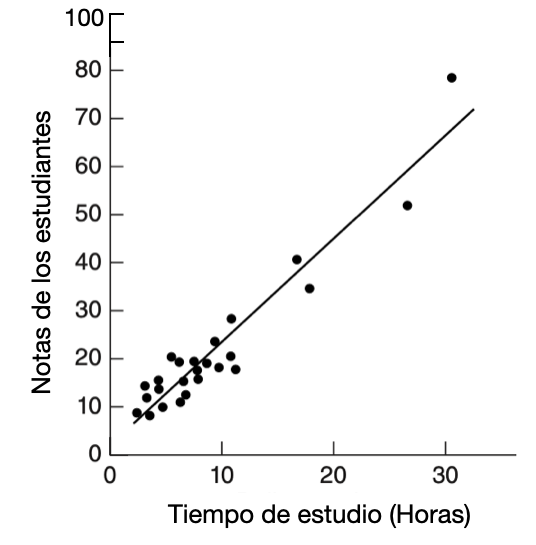
\includegraphics[height=2.5in,width=2.5in]{figuras/fig18}  \quad 
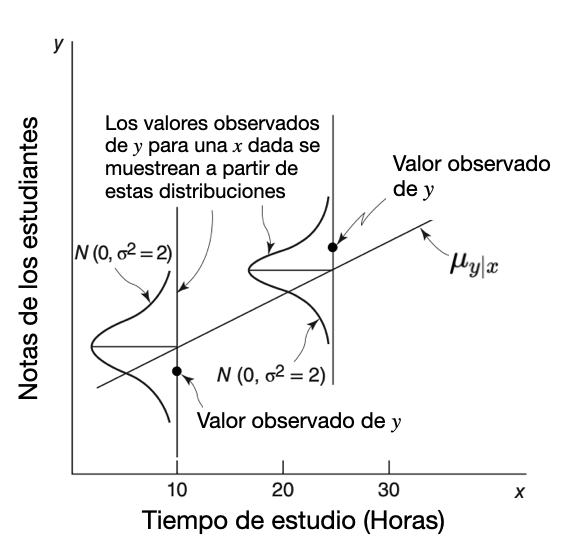
\includegraphics[height=2.6in,width=2.6in]{figuras/fig19}  
\caption{Izquierda: gr�fico de dispersi�n para las horas de estudio y las notas obtenidas. Derecha: la  generaci�n de observaciones en la regresi�n lineal.}
\label{regres1}
\end{center}
\end{figure}

Esta representaci�n sugiere  que existe una relaci�n entre el tiempo de estudio y las notas obtenidas, a medida que aumenta el n�mero de horas aumentan las notas. Adem�s, se puede apreciar que los puntos caen aproximadamente a lo largo de una l�nea recta, se dice que existe una dispersi�n de los puntos. Se puede pensar que existe una relaci�n que nos indica la tendencia de la forma
\begin{equation}
y=\beta_0+\beta_1  x \,,
\label{reglin1}
\end{equation}
donde $y$ representa las notas obtenidas, $x$ la dedicaci�n en estudio por n�mero de horas,  $\beta_0$ es la intersecci�n con el eje y $\beta_1$ es la pendiente de la recta. 

Como se puede ver, los puntos de datos no caen exactamente sobre una l�nea recta, esta dispersi�n de puntos en torno a la l�nea representa una variaci�n en el n�mero de cajas repartidas y el tiempo de entrega y es de naturaleza aleatoria. Veremos que estas  relaciones estad�sticas pueden ser muy �tiles, aunque no tengan la exactitud de una relaci�n funcional. Por lo tanto, la ecuaci�n (\ref{reglin1}) debe modificarse para tener esta caracter�stica en cuenta. 
 
Llamemos el error  $\varepsilon$ a la diferencia entre el valor observado de $y$ y la recta $\left(\beta_0+\beta_1 x\right)$. Es conveniente pensar en $\varepsilon$ como un error estad�stico; es decir, es una variable aleatoria que explica el fracaso del modelo para ajustarse exactamente a los datos. El error puede estar compuesto por los efectos de otras variables al contabilizar las horas de estudio, errores de medici�n, etc. As�, un modelo m�s plausible para los datos de las notas obtenidas es
\begin{equation}
y=\beta_0+\beta_1 x+\varepsilon
\label{reglin2}
\end{equation}

A la ecuaci�n (\ref{reglin2}) se le denomina Modelo de Regresi�n Lineal (MRL), donde normalmente a  $x$ se le denomina la variable independiente y a $y$ la variable dependiente. Esta denominaci�n puede causar  confusi�n con el concepto de independencia estad�stica, por lo que suele denominarse a $x$ como la variable ``predictora'' o ``regresora'' y a la variable $y$ como la variable de respuesta. Dado que la ecuaci�n (\ref{reglin2}) s�lo incluye una variable regresora, al modelo se le denomina Modelo de Regresi�n Lineal Simple (MRLS)




Podemos detenernos un momento para analizar el MRL, supongamos que fijamos el valor de la variable regresora $x$ y observamos el valor de la respuesta $y$. Al fijar $x$ la cantidad aleatoria $\varepsilon$ determinar� las propiedades de $y$. Supongamos que la media y la varianza de $\varepsilon$ son $0$ y $\sigma^2$, respectivamente. 

La respuesta media a cualquier valor de la variable regresora se puede escribir de la siguiente manera:
\begin{equation}
\mu_{y \mid x} \equiv E(y \mid x)=E\left(\beta_0+\beta_1 x+\varepsilon\right)=\beta_0+\beta_1 x \,,
\end{equation}
que es la misma relaci�n (\ref{reglin1}). La varianza de $y$ dado cualquier valor de $x$ es la siguiente:
\begin{equation}
\sigma_{y \mid x}^2 \equiv \operatorname{Var}(y \mid x)=\operatorname{Var}\left(\beta_0+\beta_1 x+\varepsilon\right)=\sigma^2 \,.
\end{equation}

Por lo tanto, el verdadero modelo de regresi�n $\mu_{y \mid x}=\beta_0+\beta_1 x$ es una l�nea de valores medios, es decir, la altura de la l�nea de regresi�n en cualquier valor de $x$ es s�lo el valor esperado de $y$ para ese $x$. La pendiente, $\beta_1$ puede interpretarse como el cambio en la media de $y$ para un cambio unitario en $x$. Adem�s, la variabilidad de $y$ en un valor concreto de $x$ viene determinada por la varianza del componente de error del modelo, $\sigma^2$. Esto implica que existe una distribuci�n de los valores de $y$ en cada $x$ y que la varianza de esta distribuci�n es la misma en cada $x$.

Por ejemplo, si suponemos que el verdadero modelo de regresi�n que relaciona el tiempo de estudio con las notas es $\mu_{y \mid x}=3.5+2.0 x $, y si suponemos tambi�n que la varianza es $\sigma^2=2$ entonces el resultado de estas suposiciones se puede ver en la parte derecha de la  figura \ref{regres1}. Aqu� hemos utilizado una distribuci�n normal para describir la variaci�n aleatoria de $\varepsilon$. Puesto que $y$ es la suma de una constante $\beta_0+\beta_1 x$ (la media) y una variable aleatoria $\varepsilon$ de distribuci�n normal, $y$ es una variable aleatoria de distribuci�n normal. Para el caso en que  $x=10$ horas, la nota obtenida $y$ tiene una distribuci�n normal con media $3.5+2(10)=23.5$ minutos y varianza 2. La varianza $\sigma^2$ determina la cantidad de variabilidad o ruido en las observaciones $y$ sobre el tiempo de estudio. Cuando $\sigma^2$ es peque�o, los valores observados de las notas obtenidas caer�n cerca de la recta, y cuando $\sigma^2$ es grande, los valores observados de las notas observadas  pueden desviarse considerablemente de la recta.

Notemos que pudimos haber hecho un estudio similar pero con ocho estudiantes del curso,  que elegir�amos de manera aleatoria, para entonces proceder a recopilar los datos sobre el tiempo de estudio y las calificaciones de estos estudiantes. En este caso estar�amos  haciendo lo que se llama un estudio de regresi�n muestral. Si aplic�ramos un  m�todo de regresi�n, como m�nimos cuadrados, podr�amos obtener un resultado del tipo  $\hat{y}=3.7+1.8 x$, donde los estimadores obtenidos de la muestra (estimadores muestrales) los llamaremos $m=1.8$ y $b=3.7$.  Para evaluar la precisi�n de estos  estimadores muestrales, podr�amos calcular los errores est�ndar de $m$ y $b$. Esto nos dar� una idea de cu�nto pueden variar nuestros estimadores muestrales con respecto a los verdaderos par�metros poblacionales. Por ejemplo, si calculamos el error est�ndar de $m$ y obtenemos $\Delta m=0.1$, podemos reportar el estimador muestral con su error est�ndar:
$$
m=1.8 \pm 0.1 \,.
$$
Esto significa que el verdadero valor de $m$ probablemente se encuentra en el intervalo $[1.7,1.9]$.

De alguna manera, los modelos de regresi�n pueden considerarse como modelos emp�ricos. Si la relaci�n entre las variables es muy compleja se puede utilizar regresiones lineales a trozos para aproximar la relaci�n verdadera entre las variables $y$ y $x$. En este caso las ecuaciones de regresi�n s�lo son v�lidas en la regi�n de las variables regresoras contenidas en los datos observados. 

De manera general, la variable de respuesta $y$ puede estar relacionada con un n�mero $k$ regresores, $x_1, x_2, . . . , x_k$, de forma que
\begin{equation}
y=\beta_0+\beta_1 x_1+\beta_2 x_2+\cdots+\beta_k x_k+\varepsilon
\label{reglin3}
\end{equation}

La ecuaci�n (\ref{reglin3}) se denomina Modelo de Regresi�n Lineal M�ltiple, y el adjetivo lineal se emplea para indicar que el modelo es lineal en los par�metros $\beta_0, \beta_1, \ldots, \beta_k$, no porque $y$ sea una funci�n lineal de las $x$. Esto significa que muchos modelos en los que $y$ se relaciona con las $x$ de forma no lineal pueden seguir trat�ndose como modelos de regresi�n lineal siempre que la ecuaci�n sea lineal en los $\beta$ 's.

Recordemos que el fin principal en el an�lisis de regresi�n es estimar los par�metros desconocidos del modelo de regresi�n. Este proceso tambi�n se denomina ajuste del modelo a los datos. Existen varias t�cnicas de estimaci�n de par�metros y una de estas t�cnicas es el m�todo de los m�nimos cuadrados. En el ejemplo que hemos mencionado  de las horas de estudio y las notas obtenidas por los estudiantes nos llevar�a a una ecuaci�n como la que se muestra a continuaci�n
$$
\hat{y}=3.687+ 1.821 x \,,
$$
donde $\hat{y}$  es el valor ajustado o estimado de las notas correspondiente a un valor del n�mero de horas $x$. Esta ecuaci�n ajustada es la que se  representa en la parte izquierda de la figura \ref{regres1}. Note que un estudiante que estudia cero horas $x=0$ obtendr�a una nota de $3.7$ de 100. 


Una fase importante de un an�lisis de regresi�n es la comprobaci�n de la adecuaci�n del modelo. En esta etapa, se eval�a la idoneidad del modelo y la calidad del ajuste. Este an�lisis determina la utilidad del modelo de regresi�n y puede indicar si el modelo es razonable o si necesita ser modificado. Por lo tanto, el an�lisis de regresi�n es un proceso iterativo en el que los datos gu�an la construcci�n del modelo, se ajusta el modelo a los datos y se eval�a la calidad del ajuste para decidir si se adopta o se modifica.

Es importante se�alar que un modelo de regresi�n no implica una relaci�n causa-efecto entre las variables. Una fuerte relaci�n emp�rica entre dos o m�s variables no prueba que exista una relaci�n causal entre los regresores y la respuesta. Para establecer causalidad, la relaci�n debe basarse en algo m�s all� de los datos de la muestra, como consideraciones te�ricas. El an�lisis de regresi�n puede ayudar a confirmar una relaci�n causa-efecto, pero no debe ser la �nica base para tal afirmaci�n.

Finalmente, el an�lisis de regresi�n es parte de un enfoque m�s amplio de an�lisis de datos para la resoluci�n de problemas. La ecuaci�n de regresi�n en s� puede no ser el objetivo principal del estudio; a menudo, es m�s importante entender el sistema que genera los datos.

En el trabajo de laboratorio es importante considerar la etapa que tiene que ver con la recolecci�n de los datos,  todo an�lisis de regresi�n es tan bueno como los datos en los que se basa. 

Los problemas de estimaci�n de par�metros pueden resolverse mediante m�todos de regresi�n con el objetivo de predecir la variable de respuesta. Sin embargo, al extrapolar utilizando un modelo de regresi�n para predecir eventos futuros, se corren riesgos significativos debido a los errores inherentes del modelo. Aun cuando la forma del modelo sea correcta, una estimaci�n incorrecta de los par�metros puede llevar a predicciones deficientes o incorrectas. Es esencial tener en cuenta tanto la precisi�n del modelo como la exactitud en la estimaci�n de los par�metros para minimizar estos riesgos y mejorar la fiabilidad de las predicciones.

Los modelos de regresi�n pueden utilizarse con fines de control, donde es crucial que las variables est�n relacionadas de forma causal. Sin embargo, para predicci�n, no es estrictamente necesario que exista una relaci�n causa-efecto; basta con que las relaciones presentes en los datos originales utilizados para construir la ecuaci�n de regresi�n sigan siendo v�lidas. Por ejemplo, el consumo diario de electricidad durante el mes de agosto en una ciudad puede ser un buen predictor de la temperatura m�xima diaria en agosto. No obstante, cualquier intento de reducir la temperatura m�xima disminuyendo el consumo de electricidad estar�a claramente condenado al fracaso, ya que la relaci�n entre estas variables no es causal.

\section{Los algoritmos en los modelos de regresi�n}

Desde el punto de vista computacional, la construcci�n de un modelo de regresi�n es un proceso iterativo. Los datos de entrada incluyen tanto los conocimientos te�ricos del proceso que se est� estudiando como los datos disponibles para especificar un modelo de regresi�n inicial. Las representaciones gr�ficas de los datos son muy �tiles para esta especificaci�n inicial. A continuaci�n, se estiman los par�metros del modelo, normalmente utilizando el m�todo de m�nimos cuadrados. Luego, debe evaluarse la adecuaci�n del modelo, lo que implica identificar posibles errores de especificaci�n en la forma del modelo, la omisi�n de variables importantes, la inclusi�n de variables innecesarias o la presencia de datos inusuales o inadecuados. Si el modelo resulta ser inadecuado, es necesario realizar ajustes y volver a estimar los par�metros. Este proceso puede repetirse varias veces hasta obtener un modelo adecuado. Finalmente, se debe validar el modelo para asegurarse de que producir� resultados aceptables para la aplicaci�n final.

El an�lisis de regresi�n requiere un uso inteligente y h�bil del ordenador. Un buen programa de c�lculo de regresi�n es una herramienta esencial en el proceso de creaci�n de modelos. Sin embargo, la aplicaci�n rutinaria de programas de regresi�n est�ndar no suele conducir a resultados satisfactorios. El ordenador no sustituye al pensamiento creativo sobre el problema. Debemos aprender a interpretar lo que nos dice el ordenador y a incorporar esa informaci�n en modelos posteriores. Entre la gran variedad de software estad�stico disponible, se puede mencionar el SAS (Statistical Analysis System), un paquete de software comercial para an�lisis de datos que ofrece una amplia gama de procedimientos estad�sticos, desde pruebas de hip�tesis b�sicas hasta an�lisis multivariantes complejos. Tambi�n est� R, un lenguaje de c�digo abierto y gratuito desarrollado por una comunidad global de colaboradores, conocido por su flexibilidad, extensibilidad e innovaci�n.


\section{Regresi�n lineal simple}

Un modelo con un �nico regresor $x$ y que tiene una relaci�n con la respuesta $y$ en la forma de una l�nea recta es lo que se denomina un modelo de regresi�n lineal simple:
\begin{equation}
y=\beta_0+\beta_1 x+\varepsilon \,.
\label{regrelineal}
\end{equation}

La intersecci�n $\beta_0$  y la pendiente $\beta_1$  son constantes desconocidas, mientras que $\varepsilon$ es un componente de error aleatorio. Suponemos que los errores tienen media cero y varianza desconocida $\sigma^2$. Tambi�n asumimos que los errores no est�n correlacionados, lo que significa que el valor de un error no depende del valor de ning�n otro error. Es importante considerar el regresor $x$
como controlado por el analista de datos o experimentador y medido con un error despreciable, mientras que la respuesta $y$ es una variable aleatoria. Esto implica que existe una distribuci�n de probabilidad para $y$ 
en cada valor posible de $x$.

Recordemos que la media de esta distribuci�n es:
\begin{equation}
E(y \mid x)=\beta_0+\beta_1 x\,.
\label{medireglin}
\end{equation}

Mientras que la varianza es
\begin{equation}
\operatorname{Var}(y \mid x)=\sigma^2=\operatorname{Var}\left(\beta_0+\beta_1 x+\varepsilon\right) \,.
\label{varireglin}
\end{equation}

La media de $y$ es una funci�n lineal de $x$, aunque la varianza de $y$ no depende del valor de $x$. Adem�s, como los errores no est�n correlacionados, las respuestas tampoco lo est�n. Los coeficientes de regresi�n $\beta_0$ y $\beta_1$ tienen una interpretaci�n sencilla y a menudo �til. La pendiente $\beta_1$ indica el cambio en la media de la distribuci�n de $y$ producido por un cambio unitario en $x$. Si el rango de datos de $x$ incluye $x = 0$, entonces  $\beta_0$ representa la media de la distribuci�n de la respuesta $y$ cuando $x = 0$. Si el rango de $x$ no incluye cero, entonces $\beta_0$ carece de una interpretaci�n pr�ctica.





\subsection{M�todo de los m�nimos cuadrados}

El m�todo de los m�nimos cuadrados es uno de los m�todos estad�sticos m�s usados para determinar la recta que mejor represente la tendencia de un conjunto de puntos experimentales. Como mencionamos anteriormente, los par�metros $\beta_0$ y $\beta_1$ son desconocidos y deben estimarse utilizando datos muestrales. Supongamos que tenemos $n$ pares de datos, digamos $\left(y_1, x_1\right),\left(y_2, x_2\right), \ldots,\left(y_n, x_n\right)$. Estos datos pueden proceder de un experimento controlado dise�ado espec�ficamente para recopilar los datos, de un estudio observacional o de registros hist�ricos existentes (un estudio retrospectivo).

Para estimar $\beta_0$ y $\beta_1$ utilizaremos el m�todo de los m�nimos cuadrados, esto es, estimamos $\beta_0$ y $\beta_1$ de forma que la suma de los cuadrados de las diferencias entre las observaciones $y_i$ y la recta sea un m�nimo. A partir de (\ref{regrelineal}) podemos escribir
\begin{equation}
y_i=\beta_0+\beta_1 x_i+\varepsilon_i, \quad i=1,2, \ldots, n
\label{diferencia}
\end{equation}

La ecuaci�n (\ref{regrelineal}) puede verse como un modelo de regresi�n poblacional, mientras que la ecuaci�n (\ref{diferencia}) es un modelo de regresi�n muestral, escrito en t�rminos de los $n$ pares de datos $\left(y_i, x_i\right)$, con $i=1,2, \ldots, n$. As�, el criterio de m�nimos cuadrados es
\begin{equation}
S\left(\beta_0, \beta_1\right)=\sum_{i=1}^n\left(y_i-\beta_0-\beta_1 x_i\right)^2
\end{equation}

Si la dispersi�n de los puntos experimentales es debida solo a los errores casuales en las mediciones, la mejor recta ser� aquella para la cual la suma de los cuadrados de las distancias $\left(y_i-y_0 \right)$ sea un m�nimo. Es por esto que, a este m�todo se le llama m�todo de los m�nimos cuadrados.


A los estimadores obtenidos por m�nimos cuadrados $\beta_0$ y $\beta_1$, los llamaremos $b$ y $m$, respectivamente, y deben satisfacer una relaci�n lineal de la forma:
$$
\hat{y}=m x+b \,,
$$
donde $\hat{y}$ es la variable dependiente y $x$ es la variable independiente, en nuestro caso la magnitud controlada por el experimentador. Como se ha indicado anteriormente, los valores de esas magnitudes tendr�n sus correspondientes errores que determinaremos m�s adelante. 

La desviaci�n de un valor cualquiera $y_i$ determinado experimentalmente con respecto a su valor $y_0$ en la recta, ser�:
\begin{equation}
\Delta y_i=y_i-y_0=y_i-\left(b+m x_i\right)
\label{deltay}
\end{equation}

Ahora se puede enunciar el principio b�sico de este m�todo, el cual dice que la mejor recta que puede ser trazada entre esos puntos, es aquella para la cual la suma de los cuadrados de las desviaciones $\Delta y_i$ de los datos experimentales, con respecto a esa recta, es m�nima.
$$
\sum_{i=1}^n\left(\Delta y_i\right)^2=\sum_{i=1}^n \left[y_i-b-m x_i \right]^2
$$
donde $n$ es el n�mero de pares de valores de $y$ y $x$.

Ya que la condici�n exigida es la de minimizar la suma anterior, entonces los par�metros $m$ y $b$ deben ajustarse para cumplir con esta condici�n. Ello se logra calculando las derivadas parciales de la suma con respecto a $m$ y con respecto a $b$, e igual�ndolas a cero.
$$
\begin{aligned}
& \frac{\partial\left[\sum\left(\Delta y_i\right)^2\right]}{\partial b}=
\sum_{i=1}^n\frac{\partial\left(y_i-b-m x_i \right)^2}{\partial b} = 
\sum_{i=1}^n -2(y_i-b-m x_i)=0  \\
& \frac{\partial\left[\sum\left(\Delta y_i\right)^2\right]}{\partial m}=
\sum_{i=1}^n\frac{\partial\left(y_i-b-m x_i \right)^2}{\partial m} =
\sum_{i=1}^n -2x_i(y_i-b-m x_i)=0
&
\end{aligned}
$$

Por lo tanto, se debe resolver el sistema 
$$
\begin{aligned}
&  \sum_{i=1}^n y_i - \sum_{i=1}^nb - \sum_{i=1}^n m x_i = 0  &\,\, \Rightarrow \,\,&
 nb + m \sum_{i=1}^n  x_i = \sum_{i=1}^n y_i  \\
&  \sum_{i=1}^n y_ix_i - \sum_{i=1}^n bx_i -\sum_{i=1}^n  m x_i^2 =0 & \,\, \Rightarrow \,\,&
b \sum_{i=1}^n x_i  + m \sum_{i=1}^n   x_i^2 = \sum_{i=1}^n y_ix_i
\end{aligned}
$$
para $m$ y $b$. 

Utilizando la regla de Cramer
$$
\begin{aligned}
\Delta= 
{\left|\begin{array}{cc}
n & \sum x_i \\
\sum x_i & \sum x_i^2
\end{array}\right|} = n \sum x_i^2-\left(\sum x_i\right)^2 \,,
\end{aligned}
$$
resulta:
$$
m=\frac{\left|\begin{array}{cc}
n & \sum y_i \\
\sum x_i & \sum x_i y_i
\end{array}\right|}{\Delta}=\frac{n\sum x_i y_i-\sum x_i \sum y_i}{n \sum x_i^2-\left(\sum x_i\right)^2} \quad \text{y} \quad
 b=\frac{\left|\begin{array}{cc}
\sum y_i & \sum x_i \\
\sum x_i y_i & \sum x_i^2 
\end{array}\right|}{\Delta}=\frac{\sum x_i^2 \sum y_i-\sum x_i \sum x_i y_i}{n \sum x_i^2-\left(\sum x_i\right)^2} 
$$

Por lo tanto:
\begin{eqnarray}
m &=&\dfrac{ n\sum\limits_{i=1}^n x_i y_i-\sum\limits_{i=1}^n x_i \sum\limits_{i=1}^n y_i}{n \sum\limits_{i=1}^n x_i^2-\left(\sum\limits_{i=1}^n x_i\right)^2} = 
\dfrac{\sum\limits_{i=1}^n y_i \left(x_i-\bar{x}\right)}{\sum\limits_{i=1}^n \left(x_i-\bar{x}\right)^2} 
\label{eme2} \\
b &=&\dfrac{\sum\limits_{i=1}^n x_i^2 \sum\limits_{i=1}^n y_i-\sum\limits_{i=1}^n x_i \sum\limits_{i=1}^n x_i y_i}{n\sum\limits_{i=1}^n x_i^2-\left(\sum\limits_{i=1}^n x_i\right)^2} =  \bar{y}-m \bar{x} \,,
\label{b2}
\end{eqnarray}
donde $\bar{y} \equiv \frac{1}{n} \sum_{i=1}^n y_i$ y $\bar{x} \equiv \frac{1}{n} \sum_{i=1}^n x_i$ son las medias simples.

De esta manera obtenemos la recta $\hat{y}=mx+b$ que mejor de aproxima a los puntos. N�tese que los t�rminos $\sum x_i^2$ y $\left(\sum x_i\right)^2$ no son lo mismo. Id�ntica observaci�n se debe hacer para los t�rminos $\sum x_i y_i $ y $\sum x_i \sum y_i$.

Podr�amos construir una tabla como la mostrada en \ref{tablamincua}, para as� ordenar la informaci�n y facilitar los c�lculos. Las cuatro sumas en la �ltima l�nea, son los valores necesarios para calcular $m$ y $b$. Los valores de $m$ y $b$ que se obtengan por el m�todo de los m�nimos cuadrados, deber�an ser muy pr�ximos a los obtenidos directamente utilizando el m�todo gr�fico. 
\begin{table}[h]
\begin{center}
\begin{tabular}{|c|c|c|c|}
\hline $y_i [\,\,]$ & $x_i [\,\,]$ & $x_i^2 [\,\,]$& $x_i y_i [\,\,]$ \\
\hline \hline $y_1$ & $x_1$ & $x_1^2$ & $x_1 y_1$ \\
\hline $\vdots$ & $\vdots$ & $\vdots$ & $\vdots$ \\
\hline $\vdots$ & $\vdots$ & $\vdots$ & $\vdots$ \\
\hline $y_n$ & $x_n$ & $x_n^2$ & $x_n y_n$ \\ \hline
\hline $\sum y_i$ &$\sum x_i $& $\sum x_i^2$ & $\sum x_i y_i$ \\
\hline
\end{tabular}
\end{center}
\caption{Tabla para facilitar el uso del  m�todo de m�nimos cuadrados}
\label{tablamincua}
\end{table}

Pero en la actualidad es casi de rutina utilizar alguna herramienta computacional  que permite hacer los c�lculos necesarios y los gr�ficos para el ajuste de la recta. Aunque el uso de este m�todo no nos obliga a hacer el gr�fico de la recta, por razones pedag�gicas, es conveniente hacerlo para as� observar m�s claramente las desviaciones de los puntos experimentales con respecto a la recta calculada. 

Una vez obtenido los valores de $m$ y ${b}$, es necesario calcular sus errores correspondientes $\Delta m$ y $\Delta b$. Esto lo podemos hacer calculando las desviaciones est�ndar  de la pendiente y la ordenada al origen, calculadas a partir de la distribuci�n de diferencias $\Delta y_i$, ecuaci�n (\ref{deltay}),  respecto de la mejor l�nea de ajuste.

Sea $\hat{y}_i=b+m x_i$ la predicci�n de $y$ basada en el valor $i$ de $x$. Entonces $e_i=y_i-\hat{y}_i$ representa el $i$ residuo - la diferencia entre el $i$ valor de respuesta observado y el $i$ valor de respuesta predicho por nuestro modelo lineal. Definimos la suma residual de cuadrados (RSS) como
$$
\mathrm{RSS}=e_1^2+e_2^2+\cdots+e_n^2
$$
o equivalentemente como
$$
\mathrm{RSS}=\left(y_1-b-m x_1\right)^2+\left(y_2-b-m x_2\right)^2+\cdots+\left(y_n-b-m x_n\right)^2 .
$$
\begin{table}[!t]
\begin{center}
\begin{tabular}{|c|c|c|c|}
\hline$x_i [\,\,]$ & $y_i [\,\,]$ & $y_i-m x_i-b$ & $(y_i-m x_i-b)^2$ \\
\hline \hline$x_1$ & $y_1$ & $y_1-m x_1-b$ & $\left(y_1-m x_1-b\right)^2$ \\
\hline$x_2$ & $y_2$ & $y_2-m x_2-b$ & $\left(y_2-m x_2-b\right)^2$ \\
\hline$\vdots$ & $\vdots$ & $\vdots$ & $\vdots$ \\
\hline$\vdots$ & $\vdots$ & $\vdots$ & $\vdots$ \\
\hline$x_n$ & $y_n$ & $y_n-m x_n-b$ & $\left(y_n-m x_n-b\right)^2$ \\ \hline
\hline & & & $\sum\limits_{i=1}^n \qquad \qquad \quad$ \\
\hline
\end{tabular}
\end{center}
\caption{Tabla para facilitar los c�lculos de $S_y$.}
\label{tablamincua2}
\end{table}

La diferencia entre el valor observado $y_i$ y el correspondiente valor ajustado $\hat{y}_i$ es un residuo. Matem�ticamente, el residuo $i$ es
$$
e_i=y_i-\hat{y}_i=y_i-\left(b+m x_i\right), \quad i=1,2, \ldots, n
$$

Los residuos desempe�an un papel importante en la investigaci�n de la adecuaci�n del modelo y en la detecci�n de desviaciones de los supuestos subyacentes. 

Sea SSE (Sum of Squared Errors) la suma de los cuadrados de los residuos.
$$
\mathrm{SSE} = \sum\limits_{i=1}^n e_i^2 = \sum\limits_{i=1}^n (y_i-\left(b+m x_i\right) )^2
$$

En el contexto del an�lisis de regresi�n por m�nimos cuadrados, se define la cantidad $S_y$ como la desviaci�n est�ndar de los errores, tambi�n conocida como el error est�ndar residual. Esta cantidad representa la ra�z cuadrada de la suma de los cuadrados de los errores dividida por $n-2$,  matem�ticamente es:
$$
S_y = \sqrt{\frac{\mathrm{SSE}}{n - 2}} 
$$
$S_y$ es una medida de la dispersi�n de los datos alrededor de la recta de regresi�n ajustada y se utilizada para calcular los errores est�ndar de la pendiente $\Delta m$
 y el t�rmino independiente $\Delta b$ de la regresi�n lineal.

\begin{eqnarray}
\Delta m &= \sqrt{\dfrac{n}{n \sum\limits_{i=1}^n x_i^2 - \left(\sum\limits_{i=1}^n x_i\right)^2}} \cdot S_y 
\label{Delm}\\ \nonumber  \\
\Delta b &= \sqrt{\dfrac{\sum\limits_{i=1}^n x_i^2}{n \sum\limits_{i=1}^n x_i^2 - \left(\sum\limits_{i=1}^n x_i\right)^2}} \cdot S_y
\label{Delb}
\end{eqnarray}


Finalmente para calcular $S_y$ se puede utilizar como ayuda la tabla \ref{tablamincua2}.


%example
\begin{example}
\label{ejemvelocidadtiempo}
En un experimento sobre cinem�tica un grupo de estudiantes mide los tiempos con los que se desplaza  un m�vil en un riel de aire. Los tiempos son medidos en segundos usando un cron�metro de sensibilidad $\Delta t=0,01$ s. Otro  instrumento  mide las velocidades con las que se desplaza el m�vil, este instrumento tiene una sensibilidad de $\Delta v= 0,01$ m/s.  La tabla de datos y la respectiva gr�fica se muestran la figura \ref{datosvt}.
\begin{figure}[h]
\centering
\begin{minipage}{0.54\textwidth}
    \centering
    \begin{tabular}{|c|c|}
    \hline $t_i \pm 0,01 (\mathrm{s})$ & $v_i \pm 0,01 (\mathrm{m/s})$  \\\hline \hline 
    \hline $0,00$ & 1.00 \\
    \hline $0,10$ & 1.64 \\
    \hline $0,20$ & 1.51 \\
    \hline $0,30$ & 2.03 \\
    \hline $0,40$ & 2.75 \\
    \hline $0,50$ & 3.59 \\
    \hline $0,60$ & 4.87 \\
    \hline $0,70$ & 5.23 \\
    \hline $0,80$ & 5.44 \\
    \hline $1,00$ & 6.37 \\
    \hline
    \end{tabular}
    \caption{Mediciones de la velocidad de un cuerpo en funci�n del tiempo y la gr�fica de dispersi�n respectiva.}
    \label{datosvt}
\end{minipage}
\hfill
\begin{minipage}{0.44\textwidth}
    \centering
    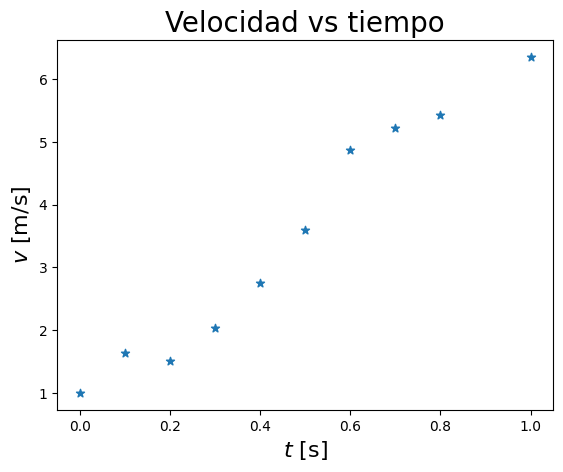
\includegraphics[height=2.6in,width=2.6in]{figuras/fig12}
\end{minipage}
\end{figure}

Como queremos  efectuar los c�lculos manualmente es recomendable calcular las siguientes sumas:
$$
\begin{array}{c|c|c|c|c}
n&\sum_{i=1}^n t_i & \sum_{i=1}^n v_i   & \sum_{i=1}^n t_i^2  & \sum_{i=1}^n t_i v_i \\ \hline\hline 
10 & 4.60 & 34.43 & 3.04 & 21.275
\end{array}
$$
$$
\Delta=n\sum\limits_{i=1}^n t_i^2-\left(\sum\limits_{i=1}^n t_i\right)^2= 
10(3.04) - \left(4.60 \right)^2= 9.24 \,\, \mathrm{s}^2
$$
$$
b=\dfrac{\sum\limits_{i=1}^n t_i^2 \sum\limits_{i=1}^n v_i-\sum\limits_{i=1}^n t_i \sum\limits_{i=1}^n t_i v_i}{\Delta} =
\frac{(3.04)  (34.43) -(4.60) (21.275)}{9.24} = 0.7362 \,\, \mathrm{m/s}
$$
$$
m =\dfrac{n \sum\limits_{i=1}^n t_i v_i-\sum\limits_{i=1}^n t_i \sum\limits_{i=1}^n v_i}{\Delta} =\frac{10(21.275)  -(4.60) ( 34.43)}{9.24}= 5.8844\,\, \mathrm{m/s^2}
$$

Procedemos a calcular la suma de los cuadrados de los residuos
$$
\begin{array}{c|c}
n& \sum\limits_{i=1}^n \left(v_i-b-m t_i\right)^2  \\ \hline\hline 
10 & 1.244  
\end{array} \,\,\Rightarrow \,\,  S_y=\left[\frac{\sum\limits_{i=1}^n \left(v_i-b-m t_i\right)^2}{n-2}\right]^{\frac{1}{2}}=
\left(\frac{1.244}{8}\right)^{\frac{1}{2}}= 0.394 \,.
$$
y los errores 
$$
\begin{aligned}
\Delta m & =\left[\frac{n}{\Delta}\right]^{\frac{1}{2}} S_y = \left[\frac{10}{9.24}\right]^{\frac{1}{2}} ( 0.394 )=0.401  \,, \\
\Delta b & =\left[\frac{\sum\limits_{i=1}^n\left(t_i\right)^2}{\Delta}\right]^{\frac{1}{2}} S_y= 
\left[\frac{3.04}{9.24}\right]^{\frac{1}{2}} ( 0.394 )= 0.226 \,. 
\end{aligned}
$$

Por lo tanto nuestro resultado ser�, por los redondeos hechos en los c�lculos
$$
v=mt + b= 5.91 t + 0.724 \,\, \mathrm{m/s}
$$
donde lo correcto ser�a escribir: $m=5.9 \pm 0.4$ y $b=0.7 \pm 0.2$.


En Python podemos hacer todos los c�lculos anteriores, incluida la figura  \ref{datosvt}.
\begin{lstlisting}[language=Python]    
import numpy as np
import matplotlib.pyplot as plt
\end{lstlisting}
Los datos:
\begin{lstlisting}[language=Python]    
yn=  array([1.000, 1.64, 1.51, 2.03, 2.75, 3.59, 4.87, 5.23, 5.44, 6.37])
xn = array([0.00, 0.10, 0.20, 0.30, 0.40, 0.50, 0.60, 0.70, 0.80, 1.00])
\end{lstlisting}

La gr�fica de la figura \ref{datosvt} se obtiene a partir de las siguientes lineas de c�digo:
\begin{lstlisting}[language=Python] 
plt.scatter(xn, yn, marker='*')
plt.title(r'Velocidad vs tiempo', fontsize=20)
plt.xlabel(r'$t$ [s]', fontsize=16)
plt.ylabel(r'$v$ [m/s]', fontsize=16)
\end{lstlisting}

Para usar las ecuaciones (\ref{eme2})-(\ref{b2}) hagamos primero los siguientes c�lculos intermedios
\begin{lstlisting}[language=Python] 
#Se obtiene el valor de n (numero de datos)
n=len(xn)
#Las sumatorias necesarias 
Sum_x = np.sum(xn)
Sum_y = np.sum(yn)
Sum_xx = np.sum(xn**2)
Sum_xy = np.sum(xn*yn)
Sum_xSumy = np.sum(xn)*np.sum(yn)
Delta = n*np.sum(xn**2) - (np.sum(xn))**2
print(n,',', Sum_x, ',',Sum_y,',', Sum_xx,',', Sum_xy,',', Sum_xSumy, ',',Delta)
\end{lstlisting}
\begin{tcolorbox}[width=\textwidth,colback={ghostwhite}]   
{\small 
10 , 4.6 , 34.43 , 3.04 , 21.275, 158.378 , 9.240000000000002
}
\end{tcolorbox} 

Y finalmente calculamos $b$ y $m$
\begin{lstlisting}[language=Python] 
# Se escriben las ecuaciones para b y m 
b=(Sum_xx*Sum_y-Sum_xy*Sum_x)/(n*Sum_xx-Sum_x**2)
m=(n*Sum_xy-Sum_x*Sum_y)/(n*Sum_xx-Sum_x**2)
print('m=',m, ',', 'b=',b)
\end{lstlisting}
\begin{tcolorbox}[width=\textwidth,colback={ghostwhite}]   
{\small 
m= 5.884415584415585 , b= 0.7361688311688325
}
\end{tcolorbox} 

Grafiquemos la recta y los datos
\begin{lstlisting}[language=Python] 
# La gr�fica con los datos y la recta que mejor se ajusta 
y_pred=m_mc*xn + b_mc
plt.figure()
plt.scatter(xn, yn, color='b',marker='+', label='datos medidos')
plt.plot(xn, y_pred, 'r--',label='recta por m�nimos cuadrados')
plt.grid(linestyle='dotted')
plt.legend(loc='best')
plt.title(r'Velocidad vs tiempo', fontsize=18)
plt.xlabel(r'$t$ [s]', fontsize=16)
plt.ylabel(r'$v$ [m/s]', fontsize=16)
plt.text(0.6, 1.0, '$y=(5.88) x + 0.736$', fontsize=12)
plt.show()
\end{lstlisting}
\begin{figure}[!h]
\begin{center}
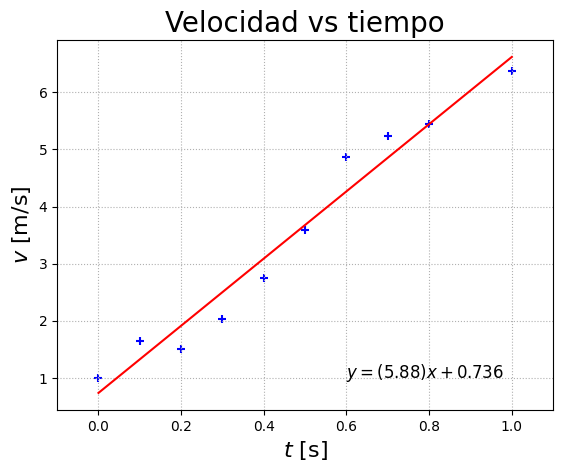
\includegraphics[height=2.6in,width=3.0in]{figuras/fig13}  
\label{figdatos2}
\end{center}
\end{figure}

El siguiente paso es calcular $\Delta b$ y $\Delta m$, pero primero $S_y$

\begin{lstlisting}[language=Python] 
SSE= np.sum((yn -(b_mc + m_mc*xn))**2)
Sy= np.sqrt(SSE/(n-2))
print('n=',n,',','SSE=', SSE ,',', 'Sy=',Sy)
\end{lstlisting}
\begin{tcolorbox}[width=\textwidth,colback={ghostwhite}]   
{\small 
n= 10 , SSE= 1.244265584415585 , Sy= 0.3943769745458628
}
\end{tcolorbox}

Los respectivos errores se obtienen de las ecuaciones (\ref{Delm}) y (\ref{Delb}) 

\begin{lstlisting}[language=Python] 
Delta_m = np.sqrt(n/(n*np.sum(xn ** 2) - np.sum(xn)**2))*Sy
Delta_b = np.sqrt(np.sum(xn**2)/(n*np.sum(xn**2)-np.sum(xn)**2))*Sy
print(f'm = {np.round(m_mc, 1)} \u00B1 {np.round(Delta_m, 1)}')
print(f'b = {np.round(b_mc, 1)} \u00B1 {np.round(Delta_b, 1)}')
\end{lstlisting}
\begin{tcolorbox}[width=\textwidth,colback={ghostwhite}]   
{\small 
$m = 5.9 \pm 0.4$

$b = 0.7 \pm 0.2$
}
\end{tcolorbox}

Por lo tanto:
$$
v= 5.9 t + 0.7 \,\, \mathrm{m/s} \,.
$$

Numpy tiene una funci�n espec�fica para calcular los par�metros $m$ y $b$, m�s informaci�n en \url{https://numpy.org/doc/stable/reference/generated/numpy.linalg.lstsq.html}

Veamos como funciona:

\begin{lstlisting}[language=Python] 
# Ajustar la recta por m�nimos cuadrados usando linalg.lstsq
A = np.vstack([xn, np.ones(len(xn))]).T
m_c, b_c = np.linalg.lstsq(A, yn, rcond=None)[0]
print(f'm = {np.round(m_c, 1)}' )
print(f'b = {np.round(b_c, 1)}' )
\end{lstlisting}
\begin{tcolorbox}[width=\textwidth,colback={ghostwhite}]   
{\small 
$m = 5.9 $

$b = 0.7 $
}
\end{tcolorbox}


Actualmente, la funci�n ``np.linalg.lstsq'' de Numpy no proporciona directamente los errores est�ndar de los coeficientes. Sin embargo, hay otras bibliotecas en Python que pueden hacer regresi�n lineal y proporcionar estos errores de manera m�s directa. Una de las bibliotecas m�s utilizadas para este prop�sito es ``statsmodels''. Para m�s informaci�n ver: \url{https://www.statsmodels.org/stable/index.html}

Veamos como funciona en nuestro ejemplo, primero cargamos la librer�a 
\begin{lstlisting}[language=Python] 
import statsmodels.api as sm
\end{lstlisting}

Luego ejecutamos las siguientes lineas de c�digo para los c�lculos

\begin{lstlisting}[language=Python] 
# Agregamos una constante (columna de unos) a xn
X = sm.add_constant(xn)
# Ajustamos el modelo
model = sm.OLS(yn, X).fit()
# Obtenemos los coeficientes y los errores est�ndar
b, m = model.params
Delta_b, Delta_m = model.bse
\end{lstlisting}

Con las siguientes lineas mostramos los resultados

\begin{lstlisting}[language=Python] 
# Imprimimos los coeficientes y sus errores est�ndar
print(f'm = {m:.4f} \u00B1 {Delta_m:.4f}')
print(f'b = {b:.4f} \u00B1 {Delta_b:.4f}')
\end{lstlisting}
\begin{tcolorbox}[width=\textwidth,colback={ghostwhite}]   
{\small 
$m = 5.8844 \pm 0.4103$

$b = 0.7362 \pm 0.2262$
}
\end{tcolorbox}

Y ahora la gr�fica
\begin{lstlisting}[language=Python] 
# Generamos valores de y usando los coeficientes obtenidos
y_pred = m * xn + b
# Graficamos los datos originales y la l�nea ajustada
plt.scatter(xn, yn, color='blue', label='Datos originales')
plt.plot(xn, y_pred, color='red', label='L�nea ajustada')
plt.xlabel('x')
plt.ylabel('y')
plt.legend()
plt.show()
\end{lstlisting}
\begin{figure}[!h]
\begin{center}
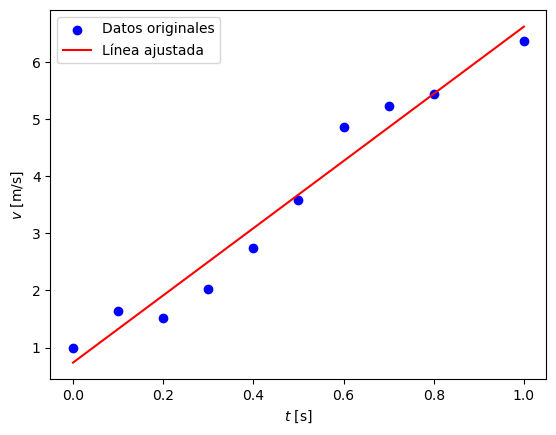
\includegraphics[height=2.6in,width=3.0in]{figuras/fig20}  
\label{figdatos2}
\end{center}
\end{figure}
\end{example}
\exampleline

\subsection{Propiedades del m�todo de m�nimos cuadrados}

Podemos notar de la ecuaci�n (\ref{eme2})
$$
m  = \dfrac{\sum\limits_{i=1}^n y_i \left(x_i-\bar{x}\right)}{\sum\limits_{i=1}^n \left(x_i-\bar{x}\right)^2} =\sum_{i=1}^n c_i y_i \,,\quad \text{donde} \quad c_i = \frac{\left(x_i-\bar{x}\right)}{\sum\limits_{i=1}^n \left(x_i-\bar{x}\right)^2}
\label{eme3}
$$

Se dice que los estimadores $m$ y $b$ por m�nimos cuadrados son estimadores no ambiguos porque
$$
\begin{aligned}
E\left(m\right)  =E\left(\sum_{i=1}^n c_i y_i\right)=\sum_{i=1}^n c_i E\left(y_i\right)  =\sum_{i=1}^n c_i\left(\beta_0+\beta_1 x_i\right)=\beta_0 \sum_{i=1}^n c_i+\beta_1 \sum_{i=1}^n c_i x_i
\end{aligned}
$$
ya que por suposici�n $E\left(\varepsilon_i\right)=0$. Se puede demostrar que $\sum_{i=1}^n c_i=0$ y $\sum_{i=1}^n c_i x_i=1$, por lo que
$$
E\left(m \right)=\beta_1
$$

Es decir, si suponemos que el modelo es correcto $\left[E\left(y_i\right)=\beta_0+\beta_1 x_i\right]$, entonces $m$ es un estimador no sesgado de $\beta_1$. Del mismo modo podemos demostrar que $b$ es un estimador no sesgado de $\beta_0$, o bien
$$
E\left(b\right)=\beta_0 \,.
$$


%example
\begin{example}
\label{ejemcizalla}
Una pega para piezas met�licas se prueba mediante una fuerza de cizallamiento entre las partes. La resistencia al cizallamiento de la uni�n entre los dos tipos de piezas es una caracter�stica crucial de calidad. Se observa que, con el transcurso del tiempo, la pega se debilita, lo cual es un problema que los ingenieros deben resolver. Los datos muestran esta relaci�n con la edad de aplicaci�n de la pega, medida en semanas. Se han recogido veinte observaciones sobre la resistencia al cizallamiento y la edad de la pega, como se muestra en la tabla \ref{datosciza}. Un diagrama de dispersi�n sugiere una fuerte relaci�n estad�stica entre la resistencia al cizallamiento y la edad del pegamento. La hip�tesis inicial de un modelo lineal, $y=\beta_0+\beta_1 x+\varepsilon$, parece razonable. 
\begin{figure}[h]
\begin{tabular}{ccc}
\hline Observaci�n, $i$ & \begin{tabular}{c} 
Cizallamiento, $y_i ( \mathrm{psi} )$
\end{tabular} & \begin{tabular}{c} 
Edad de la pega, $x_i ($ semanas $)$
\end{tabular} \\
\hline 1 & 2158.70 & 15.50 \\
2 & 1678.15 & 23.75 \\
3 & 2316.00 & 8.00 \\
4 & 2061.30 & 17.00 \\
5 & 2207.50 & 5.50 \\
6 & 1708.30 & 19.00 \\
7 & 1784.70 & 24.00 \\
8 & 2575.00 & 2.50 \\
9 & 2357.90 & 7.50 \\
10 & 2256.70 & 11.00 \\
11 & 2165.20 & 13.00 \\
12 & 2399.55 & 3.75 \\
13 & 1779.80 & 25.00 \\
14 & 2336.75 & 9.75 \\
15 & 1765.30 & 22.00 \\
16 & 2053.50 & 18.00 \\
17 & 2414.40 & 6.00 \\
18 & 2200.50 & 12.50 \\
19 & 2654.20 & 2.00 \\
20 & 1753.70 & 21.50 \\
\hline
\end{tabular}
\label{datosciza}
\caption{Datos para el ejemplo \ref{ejemcizalla}.}
\end{figure}

A continuaci�n haremos los c�lculos directamente con Python y la librer�a ``statsmodels'' ya usada en el ejemplo \ref{ejemvelocidadtiempo}. Primero los datos de la tabla \ref{datosciza}
\begin{lstlisting}[language=Python] 
 # Datos de cizallamiento y edad de la pega
xn = np.array([15.50, 23.75, 8.00, 17.00, 5.50, 19.00, 24.00, 2.50,
                      7.50, 11.00, 13.00, 3.75, 25.00, 9.75, 22.00, 18.00,
                      6.00, 12.50, 2.00, 21.50])
yn = np.array([2158.70, 1678.15, 2316.00, 2061.30, 2207.50,
                          1708.30, 1784.70, 2575.00, 2357.90, 2256.70,
                          2165.20, 2399.55, 1779.80, 2336.75, 1765.30,
                          2053.50, 2414.40, 2200.50, 2654.20, 1753.70])
\end{lstlisting}

Luego hacemos el c�lculo de los par�metros $m$ y $b$
\begin{lstlisting}[language=Python] 
X = sm.add_constant(xn)
# Ajustamos el modelo
model = sm.OLS(yn, X).fit()
# Obtenemos los coeficientes y los errores est�ndar
b, m = model.params
Delta_b, Delta_m = model.bse
# Imprimimos los coeficientes y sus errores est�ndar
print(f'm = {m:.4f} \u00B1 {Delta_m:.4f}')
print(f'b = {b:.4f} \u00B1 {Delta_b:.4f}')
\end{lstlisting}
\begin{tcolorbox}[width=\textwidth,colback={ghostwhite}]   
{\small 
$m = -37.1536 \pm 2.8891$

$b = 2627.8224 \pm 44.1839$
}
\end{tcolorbox}

Y la gr�fica con los datos y la recta obtenida
\begin{lstlisting}[language=Python] 
# Generamos valores de y usando los coeficientes obtenidos
y_pred = m * xn + b
# Graficamos los datos originales y la l�nea ajustada
plt.scatter(xn, yn, color='blue', label='Datos')
plt.plot(xn, y_pred, color='red', label='L�nea ajustada')
plt.grid(linestyle='dotted')
plt.legend(loc='best')
plt.xlabel('Edad de la pega (semanas)')
plt.ylabel('Fuerza de cizallamiento (psi)')
plt.legend()
plt.show()
\end{lstlisting}
\begin{figure}[!h]
\begin{center}
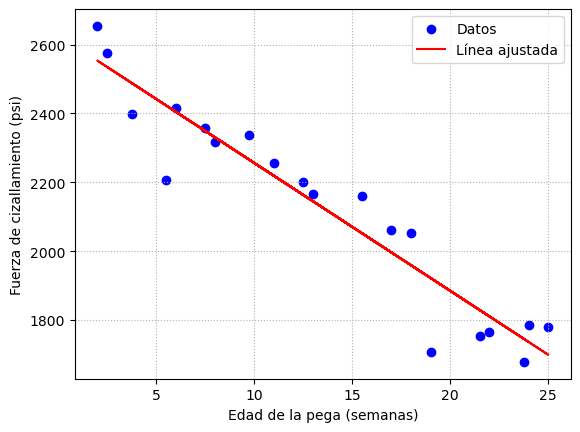
\includegraphics[height=2.6in,width=3.0in]{figuras/fig21}  
\label{figdatos2}
\end{center}
\end{figure}

La recta tiene por ecuaci�n
$$
\hat{y}=2627.82-37.15 x \,.
$$
Recordemos que la pendiente $-37.15$ se interpreta como la disminuci�n media semanal de la resistencia al cizallamiento debida a la edad de la pega. Dado que el l�mite inferior de las $x$ est� cerca del origen, el intercepto $ 2627.82$ representa la resistencia al corte en un lote de muestra inmediatamente despu�s de la aplicaci�n de la pega. 

Veamos los valores ajustados $\hat{y}$ obtenidos
\begin{lstlisting}[language=Python] 
y_pred = m * xn + b
y_pred
\end{lstlisting}
\begin{tcolorbox}[width=\textwidth,colback={ghostwhite}]   
{\small 
array([2051.94169936, 1745.42457406, 2330.59363144, 1996.21131294,
       2423.4776088 , 1921.90413105, 1736.13617632, 2534.93838164,
       2349.17042691, 2219.13285861, 2144.82567672, 2488.49639296,
       1698.98258538, 2265.57484729, 1810.44335821, 1959.05772199,
       2404.90081333, 2163.40247219, 2553.51517711, 1829.02015369])
}
\end{tcolorbox}
y tambi�n los residuos
\begin{lstlisting}[language=Python] 
e_i=yn-y_pred
e_i
\end{lstlisting}
\begin{tcolorbox}[width=\textwidth,colback={ghostwhite}]   
{\small 
array([ 106.75830064,  -67.27457406,  -14.59363144,   65.08868706,
       -215.9776088 , -213.60413105,   48.56382368,   40.06161836,
          8.72957309,   37.56714139,   20.37432328,  -88.94639296,
         80.81741462,   71.17515271,  -45.14335821,   94.44227801,
          9.49918667,   37.09752781,  100.68482289,  -75.32015369])
}
\end{tcolorbox}

Hay varias propiedades de los m�nimos cuadrados que podemos probar:


1)  La suma de los valores observados $y_i$ es igual a la suma de los valores ajustados $\hat{y}_i$, o bien
$$
\sum_{i=1}^n y_i=\sum_{i=1}^n \hat{y}_i
$$
El lado izquierdo de la ecuaci�n es:
\begin{lstlisting}[language=Python] 
Sum_y = np.sum(yn)
Sum_y 
\end{lstlisting}
\begin{tcolorbox}[width=\textwidth,colback={ghostwhite}]   
{\small 
42627.149999999994
}
\end{tcolorbox}
Y el lado derecho:
\begin{lstlisting}[language=Python] 
Sum_yp = np.sum(y_pred)
Sum_yp
\end{lstlisting}
\begin{tcolorbox}[width=\textwidth,colback={ghostwhite}]   
{\small 
42627.149999999965
}
\end{tcolorbox}

2) La suma de los residuos en cualquier modelo de regresi�n que contiene un intercepto $\beta_0$ es siempre cero, es decir,
$$
\sum_{i=1}^n\left(y_i-\hat{y}_i\right)=\sum_{i=1}^n e_i=0
$$

\begin{lstlisting}[language=Python] 
np.sum(e_i)
\end{lstlisting}
\begin{tcolorbox}[width=\textwidth,colback={ghostwhite}]   
{\small 
3.069544618483633e-11
}
\end{tcolorbox}
Es decir, $\sum e_i=0.00$. 

3)  La recta de regresi�n por m�nimos cuadrados siempre pasa por el centroide, el punto $(\bar{x}, \bar{y})$ de los datos.
$$
\bar{x} = \frac{1}{n}\sum_{i=1}^n  x_i \,, \quad  \bar{y} = \frac{1}{n}\sum_{i=1}^n  y_i= m\bar{x} +b \,. 
$$
\begin{lstlisting}[language=Python] 
# Los promedios de x y y 
xp =np.sum(xn)/len(xn) 
yp=np.sum(yn)/len(xn)
# Se imprimen los promedios y la recta evaluada en xp
print(xp,',', yp,',', m * xp + b)
\end{lstlisting}
\begin{tcolorbox}[width=\textwidth,colback={ghostwhite}]   
{\small 
13.3625 , 2131.3574999999996 , 2131.3574999999983
}
\end{tcolorbox}

4) La suma de los residuos ponderada por el valor correspondiente de la variable regresora siempre es igual a cero, es decir,
$$
\sum_{i=1}^n x_i e_i=0
$$
\begin{lstlisting}[language=Python] 
np.sum(xn*e_i)
\end{lstlisting}
\begin{tcolorbox}[width=\textwidth,colback={ghostwhite}]   
{\small 
4.2746250983327627e-10
}
\end{tcolorbox}

5) La suma de los residuos ponderada por el valor ajustado correspondiente siempre
es igual a cero, es decir
$$
\sum_{i=1}^n \hat{y}_i e_i=0
$$
\begin{lstlisting}[language=Python] 
np.sum(y_pred*e_i)
\end{lstlisting}
\begin{tcolorbox}[width=\textwidth,colback={ghostwhite}]   
{\small 
6.478512659668922e-08
}
\end{tcolorbox}


Los programas estad�sticos suelen ofrecer un resumen de todos los c�lculos que realiza el programa. La salida en pantalla o consola de la figura \ref{figejemciza} presenta los resultados de la librer�a ``statsmodels''  para el ejemplo que estamos considerando. La parte superior de la tabla contiene el modelo de regresi�n ajustado. Observe que, antes del redondeo, los coeficientes de regresi�n coinciden con los que calculamos manualmente. La salida en pantalla mostrada el la figura \ref{figejemciza} tambi�n contiene otra informaci�n sobre el modelo de regresi�n que pueden ser consultadas en el manual de la librer�a. 

\begin{lstlisting}[language=Python] 
results = model
print(results.summary())
\end{lstlisting}
\begin{figure}[!h]
\begin{center}
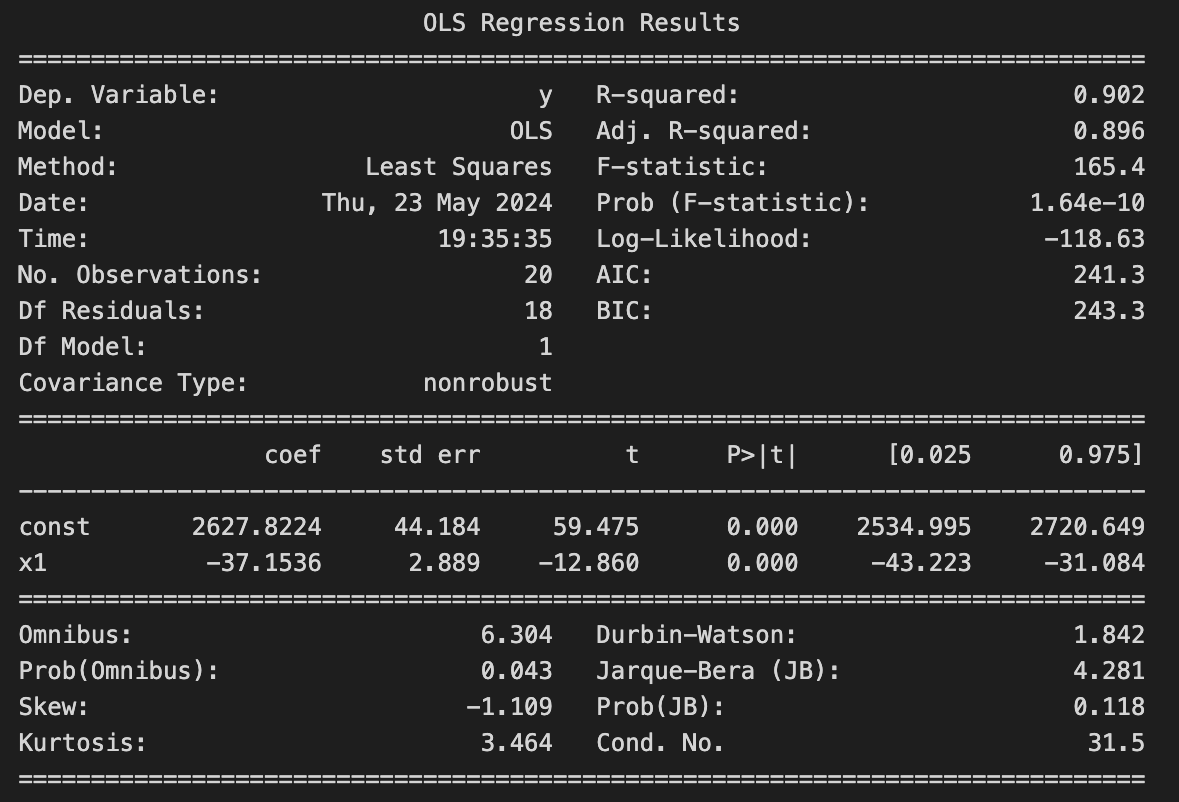
\includegraphics[height=4.0in,width=6.4in]{figuras/fig22}  
\caption{Resumen de las estimaciones estad�sticas por consola.}
\label{figejemciza}
\end{center}
\end{figure}

\end{example}
\exampleline


\subsubsection{La estimaci�n de $\sigma^2$}

Adem�s de estimar $\beta_0$ y $\beta_1$, se necesita una estimaci�n de la varianza del error $\sigma^2$, que  proporciona informaci�n crucial sobre la variabilidad de los errores (residuos) y tiene varias aplicaciones en el an�lisis estad�stico como  probar hip�tesis y construir estimaciones de intervalo pertinentes para el modelo de regresi�n. Lo ideal ser�a que esta estimaci�n no dependiera de la adecuaci�n del modelo ajustado. Esto s�lo es posible cuando hay varias observaciones de $y$ para al menos un valor de $x$  o cuando se dispone de informaci�n previa sobre $\sigma^2$. Cuando no se puede utilizar este enfoque, la estimaci�n de $\sigma^2$ se obtiene a partir de la suma de cuadrados de los  errores:
\begin{equation}
\hat{\sigma}^2=\sum_{i=1}^n e_i^2=\sum_{i=1}^n\left(y_i-\hat{y}_i\right)^2 \,.
\end{equation}

Conocidos los valores estimados de $\beta_0$ y $\beta_1$, es decir: $
\hat{y}_i=b+m x_i $ y al sustituir en la ecuaci�n anterior
\begin{equation}
\hat{\sigma}^2=\sum_{i=1}^n\left(y_i - b-m x_i \right)^2 = 
\sum_{i=1}^n\left(y_i - \bar{y}+m\bar{x} -m x_i \right)^2 = 
\sum_{i=1}^n\left(y_i - \bar{y}+m(\bar{x} - x_i) \right)^2 
\end{equation}

\begin{equation}
\sum_{i=1}^n y_i^2-n \bar{y}^2-\hat{\beta}_1 \sum_{i=1}^n y_i\left(x_i-\bar{x}\right)
\end{equation}

$$
=\sum_{i=1}^n y_i\left(x_i-\bar{x}\right)
$$

$b=\bar{y}-m\bar{x}$




\chapter{�C�mo escribir un informe de laboratorio?}

\section{Introducci�n}

La �ltima secci�n se enfocar� en las pautas y estructura para la redacci�n de informes de laboratorio. Se proporcionar�n consejos sobre la organizaci�n de la informaci�n, la inclusi�n de resultados, tablas y gr�ficos, la elaboraci�n de conclusiones y la citaci�n adecuada de fuentes.




Describir en un texto el trabajo de una investigaci�n para que sea comprensible para los dem�s y aceptable para su publicaci�n es una tarea que puede resultar  dif�cil y escabrosa. Por eso es necesario que los estudiantes universitarios aprendan a implicarse en esta tarea desde sus primeros contactos con los laboratorios. 

En este contexto universitario el  informe o monograf�a de laboratorio es un texto que se basa en las experiencias obtenidas en el laboratorio, o de una investigaci�n te�rica, que pretender ser una primera aproximaci�n a las publicaciones cient�ficas profesionales. 

La idea principal es que el estudiante y futuro investigador comunique sus resultados, logros y avances  de la mejor manera posible, con la suficiente precisi�n y claridad como para que otros investigadores o estudiantes puedan interpretar tambi�n los resultados, incluso replicar la experiencia. 

Por lo tanto, es importante que el estudiante comience a familiarizarse con el m�todo cient�fico y que sea capaz, no solo  de relacionar la teor�a con los resultados experimentales, sino que tambi�n sea capaz de comunicar su experiencia de manera satisfactoria. 

\section{Estructura}
Un reporte, informe o monograf�a debe estar conformado por  conjunto de partes o secciones que son esenciales para su elaboraci�n. B�sicamente son las que se muestra a continuaci�n:
\begin{enumerate}
\item Resumen: El resumen debe tener el contenido suficiente para que el lector se construya una idea completa de qu� se hizo y cu�les fueron los resultados. 

\item Introducci�n: Aqu� se explica la raz�n de ser del art�culo y su contexto. Se debe describir el problema, los antecedentes y la justificaci�n del trabajo. 

\item Metodolog�a: Aqu� se hace referencia a los recursos materiales que se utilizaron en el trabajo, las t�cnicas utilizadas,  la descripci�n de c�mo se realiz� el trabajo. Esta secci�n  es importante ya que debe garantizar que otra persona que lea el trabajo  pueda replicar el experimento o los c�lculos que se realizaron. 

\item Experimento y resultados: se exponen los datos obtenidos, los c�lculos que se realizaron. Tambi�n se puede asomar algunos avances sobre las ideas que se discutir�n con mayor profundidad en la conclusiones pero sin entrar en an�lisis num�ricos. 

\item Discusi�n y conclusiones: Se hace un an�lisis de los resultados obtenidos y de su relevancia, se pueden hacer comparaciones con otros trabajos, hacer predicciones, comprobar objetivos. 

\item Referencias: se escribe la lista completa de las referencias que se citaron en el texto. 
Es recomendable apegarse a un est�ndar de referencias ya que los estilos pueden variar dependiendo del �rea cient�fica o el tipo de publicaci�n. 
\end{enumerate}


\section{Modelo para un informe de laboratorio}

A continuaci�n y a manera de ap�ndice se anexa un modelo de informe de laboratorio para ser completado con la informaci�n correspondiente. 

La fuente en \LaTeX{} del documento\footnote{Art�culo realizado por el Prof Luis A. N��ez de la Escuela de F�sica} la pueden encontrar en \url{https://github.com/hectorfro/CursosUIS/tree/main/LabFisII23B}









\end{document}